\documentclass[a4paper,11pt]{article}



\usepackage{cmap}
\usepackage[T1]{fontenc}
\usepackage[utf8]{inputenc}
\input{glyphtounicode}
\pdfgentounicode=1

\usepackage{csquotes}
\usepackage[authoryear,round]{natbib}
\usepackage[french]{babel}
\usepackage{indentfirst} % Pour forcer l'alinéa au premier paragraphe
\usepackage{geometry}
\usepackage{hyperref}
\usepackage{xcolor}
\usepackage{graphicx}
\usepackage{fancyhdr}
\usepackage{array}
\usepackage{booktabs}
\usepackage{enumitem}
\usepackage{tikz}
\usetikzlibrary{positioning,arrows.meta,shapes.geometric,shapes.misc,calc}
\usepackage{pgfplots}

\usepackage[expansion=false]{microtype}
\usepackage{amsmath}
\usepackage{amssymb} % Pour \checkmark et \square
\usepackage{pifont} % Pour \ding{51} (coche) et \ding{55} (croix)

% Formatage des titres de section pour afficher "Chapitre X"
\usepackage{titlesec}
\titleformat{\section}
  {\normalfont\Large\bfseries}{Chapitre \thesection~--}{1em}{}
\usepackage{float}
\usepackage{wrapfig}
\usepackage{caption}

% Symboles pratiques pour tableaux
\newcommand{\oui}{\textcolor{black!70}{\checkmark}}
\newcommand{\non}{\textcolor{black!70}{$\times$}}

\addto\captionsfrench{\renewcommand{\contentsname}{Sommaire}}

\geometry{
  a4paper,
  left=2.5cm,
  right=2.5cm,
  top=2.5cm,
  bottom=2.5cm,
  centering
}

\setlength{\headheight}{15pt}
\setlength{\headsep}{12pt}
\hypersetup{hidelinks}

\renewcommand{\sectionmark}[1]{\markright{#1}}
\fancyhf{}
\fancyhead[R]{\nouppercase{\rightmark}}
\fancyfoot[C]{\thepage}
\renewcommand{\headrulewidth}{0pt}
\renewcommand{\footrulewidth}{0.4pt}
\fancypagestyle{plain}{%
  \fancyhf{}
  \fancyhead[R]{\nouppercase{\rightmark}}
  \fancyfoot[C]{\thepage}
  \renewcommand{\headrulewidth}{0pt}
  \renewcommand{\footrulewidth}{0.4pt}
}

\newcommand{\titreEtude}{Développement d'un outil permettant le traitement et l'insertion des archives numériques sur Geofoncier au sein d'un cabinet de Géomètre-Expert}
\newcommand{\auteur}{TRAVAILLÉ Adrien}
\newcommand{\specialite}{INSA Strasbourg - Spécialité Topographie}
\newcommand{\structure}{Cabinet de Géomètre-Expert (structure d'accueil : GEO-SIAPP)}
\newcommand{\encadrement}{Encadrant : Mathieu KOEHL}
\newcommand{\dateRapport}{2026}

\title{\textbf{Mémoire de fin d'études (PFE)}\\[0.4em]\large \titreEtude}
\author{\auteur\\\specialite\\\structure\\\encadrement}
\date{\dateRapport}

\begin{document}

\begin{titlepage}
  \thispagestyle{empty}
  \noindent% <-- important : le % supprime l'espace parasite
  \begin{minipage}[c]{0.45\textwidth}
    
\includegraphics[height=2.8cm]{Logo_INSAStrasbourg.jpg}
  \end{minipage}% <-- important : supprime le saut de ligne
  \hfill
  \begin{minipage}[c]{0.45\textwidth}
    \raggedleft
    
\includegraphics[height=2.8cm]{Geosiapp.jpg}
  \end{minipage}

  \vspace{4em}
  \begin{center}
    {\Huge\bfseries\sffamily Mémoire de fin d'études\par}
    \vspace{0.6em}
    {\Large\bfseries\sffamily (PFE)\par}
    \vspace{1em}
    
    {\rule{0.35\linewidth}{1pt}\par}
    \vspace{2.5em}
    
    
    % Mise en valeur du titre : en gras, plus grand, et bien espacé
    {\LARGE\bfseries \titreEtude\par}
    
    \vspace{3.5em}
    {\large \textbf{\auteur}\par}
    \vspace{0.5em}
    {\large \specialite\par}
    {\large \structure\par}
    {\large \encadrement\par}
    \vfill
    {\large \dateRapport\par}
  \end{center}
\end{titlepage}

\cleardoublepage
\pagenumbering{gobble}
\pdfbookmark[1]{\contentsname}{toc}

% - Pages liminaires (sans numérotation arabe) -
% !TeX root = main.tex

\phantomsection
\section*{Résumé}
\addcontentsline{toc}{section}{Résumé}

Les cabinets de géomètre-expert disposent, au fil des décennies, d'un fonds d'archives considérable composé de plans de bornage, procès-verbaux et documents d'arpentage sous des formats très hétérogènes, tous à caractère foncier. Une grande partie de ce patrimoine, produit avant la généralisation des outils numériques, demeure non indexée et non versée sur la plateforme de référence de la profession, Géofoncier. Ce travail vise à concevoir et à déployer un outil automatisé pour traiter ces archives au sein du cabinet GEO-SIAPP, en Ardèche, en vue de leur versement sur la plateforme nationale Géofoncier.

L'outil développé repose sur une chaîne de traitement
articulée autour de quatre étapes : la classification automatique du document entrant, l'extraction des informations clés (commune, date, numéro de document d'arpentage), la fiabilisation des données par croisement avec des référentiels officiels, et la préparation au versement sur Géofoncier. Pour faire face à la grande variabilité des documents et plans cadastraux récents, registres manuscrits anciens, images numérisées, l'architecture mobilise des techniques issues de la vision par ordinateur, de la reconnaissance de texte manuscrit et de l'intelligence artificielle.

Une interface de validation permet aux opérateurs de contrôler et corriger les résultats de la machine avant tout versement définitif, assurant ainsi la qualité de la donnée foncière produite et le respect des obligations déontologiques de la profession.

\vspace{1.5em}
\noindent\textbf{Mots-clés :} archivage numérique, reconnaissance de texte manuscrit (HTR), traitement automatisé, Géofoncier, intelligence artificielle, géomètre-expert, vision par ordinateur.

{\let\thefootnote\relax\footnotetext{\footnotesize Ce rapport a fait l'objet d'une relecture et d'une correction orthographique et grammaticale assistées par intelligence artificielle.}}

\clearpage

\section*{Abstract}
\addcontentsline{toc}{section}{Abstract}

Land surveying firms build up, over decades, a large archive of boundary delimitation plans, survey reports and cadastral documents in highly heterogeneous formats. A significant part of this documentary heritage, produced before digital tools became widely used, remains unindexed and has not been uploaded to Geofoncier, the profession's national platform. This work aims to design and deploy an automated archive processing tool within the GEO-SIAPP firm in Ardèche, France, in order to feed this data into the national Geofoncier platform.

The developed tool relies on a modular processing chain built around four steps: automatic classification of incoming documents, extraction of key information (municipality, date, cadastral survey number), data validation by cross-referencing official databases, and preparation for submission to Geofoncier. To handle the high variability of the documents, recent cadastral plans (old handwritten registers, degraded scanned images) the architecture combines techniques from computer vision, handwritten text recognition and generative artificial intelligence.

A validation interface allows operators to review and correct the machine's results before the final submission, guaranteeing the quality of the land data produced and compliance with the profession's ethical obligations.

\vspace{1.5em}
\noindent\textbf{Keywords:} digital archiving, handwritten text recognition (HTR), automated processing, Geofoncier, artificial intelligence, land surveyor, computer vision.

\clearpage
% !TeX root = main.tex
\phantomsection
\section*{Remerciements}
\addcontentsline{toc}{section}{Remerciements}

Ces remerciements s'adressent à toutes les personnes qui ont contribué, peu importe leur niveau d'implication, à ce projet de fin d'études.

Je tiens tout d'abord à remercier Monsieur Gaëtan HAGUE, mon tuteur de projet pour la proposition du sujet, sa confiance et son temps tout au long de ce projet. Ce dernier m'a laissé mener à bien ce projet en autonomie, m'accordant sa confiance sur le bon déroulement de l'étude, tout en me donnant des objectifs clairs et en contrôlant la direction prise durant ces six mois.

Je remercie également Monsieur Hugo DEVOS, qui m'a beaucoup aidé notamment pour la compréhension des documents en possession de l'entreprise, et pour son aide concernant son fonctionnement interne.

Je remercie aussi Monsieur Mathieu KOEHL, encadrant de ce PFE à l'INSA Strasbourg, pour ses retours et ses redirections notamment au début du projet, ainsi que l'ensemble du corps enseignant pour ces trois années de formation.

J'aimerais aussi remercier plus généralement tout le personnel du bureau GEO-SIAPP pour leur accueil et l'ambiance de travail qu'ils ont su mettre en place dès mon arrivée.

Enfin, merci à ma famille et à mes proches pour leur soutien constant durant cette dernière année de formation.

\clearpage

% !TeX root = main.tex

\section*{Liste des sigles et abréviations}
\addcontentsline{toc}{section}{Liste des sigles et abréviations}

\begin{description}[leftmargin=3cm, style=nextline]
    \item[API] Application Programming Interface
    \item[CAO] Conception Assistée par Ordinateur
    \item[COG] Code Officiel Géographique
    \item[CPU] Central Processing Unit
    \item[DA] Document d'arpentage
    \item[DMPC] Document modificatif du parcellaire cadastral
    \item[DPI] Dots Per Inch
    \item[GLiNER] Generalist and Lightweight Named Entity Recognition
    \item[GPU] Graphics Processing Unit
    \item[HTR] Handwritten Text Recognition
    \item[IHM] Interface Homme-Machine
    \item[INSEE] Institut national de la statistique et des études économiques
    \item[JSON] JavaScript Object Notation
    \item[JWT] JSON Web Token
    \item[OCR] Optical Character Recognition
    \item[OGE] Ordre des géomètres-experts
    \item[PCI] Plan cadastral informatisé
    \item[PV] Procès-verbal
    \item[REST] Representational State Transfer
    \item[RFU] Référentiel foncier unifié
    \item[RGPD] Règlement général sur la protection des données
    \item[VLM] Vision-Language Model
    \item[YOLO] You Only Look Once
\end{description}

\clearpage

\tableofcontents
\clearpage

% - Corps du mémoire -
\pagestyle{fancy}
\pagenumbering{arabic}
\setcounter{page}{1}

% !TeX root = main.tex

\section{Introduction}

\subsection{Présentation de la structure d'accueil}

Le cabinet GEO-SIAPP est une société de géomètres-experts dont le siège est implanté à Aubenas, en Ardèche, depuis 1992. Ce territoire est particulièrement vaste et à forte dominante rurale, ce qui nécessite une proximité constante avec le terrain et la clientèle. Pour couvrir ce territoire, GEO-SIAPP s'est développé autour de quatre agences, comme le montre la figure~\ref{fig:carte_agences} : Aubenas, Pierrelatte, Vallon-Pont-d'Arc et Guilherand-Granges.

Au fil de sa croissance, GEO-SIAPP a acquis plusieurs études de géomètres-experts locales. Ces acquisitions ont intégré de nouveaux collaborateurs mais aussi les archives de ces structures, dont certaines datent de plusieurs décennies. Le cabinet conserve ainsi une grande quantité de documents anciens, et pour la plupart manuscrits.

L'entreprise intervient sur l'ensemble des missions de la profession : le foncier (bornage, division parcellaire, mise en copropriété), l'urbanisme réglementaire, l'ingénierie VRD (maîtrise d'œuvre pour la voirie et les réseaux divers) ainsi que la topographie (photogrammétrie, relevés par drone,bathymétrie et scanner laser 3D).

\begin{figure}[H]
  \centering
  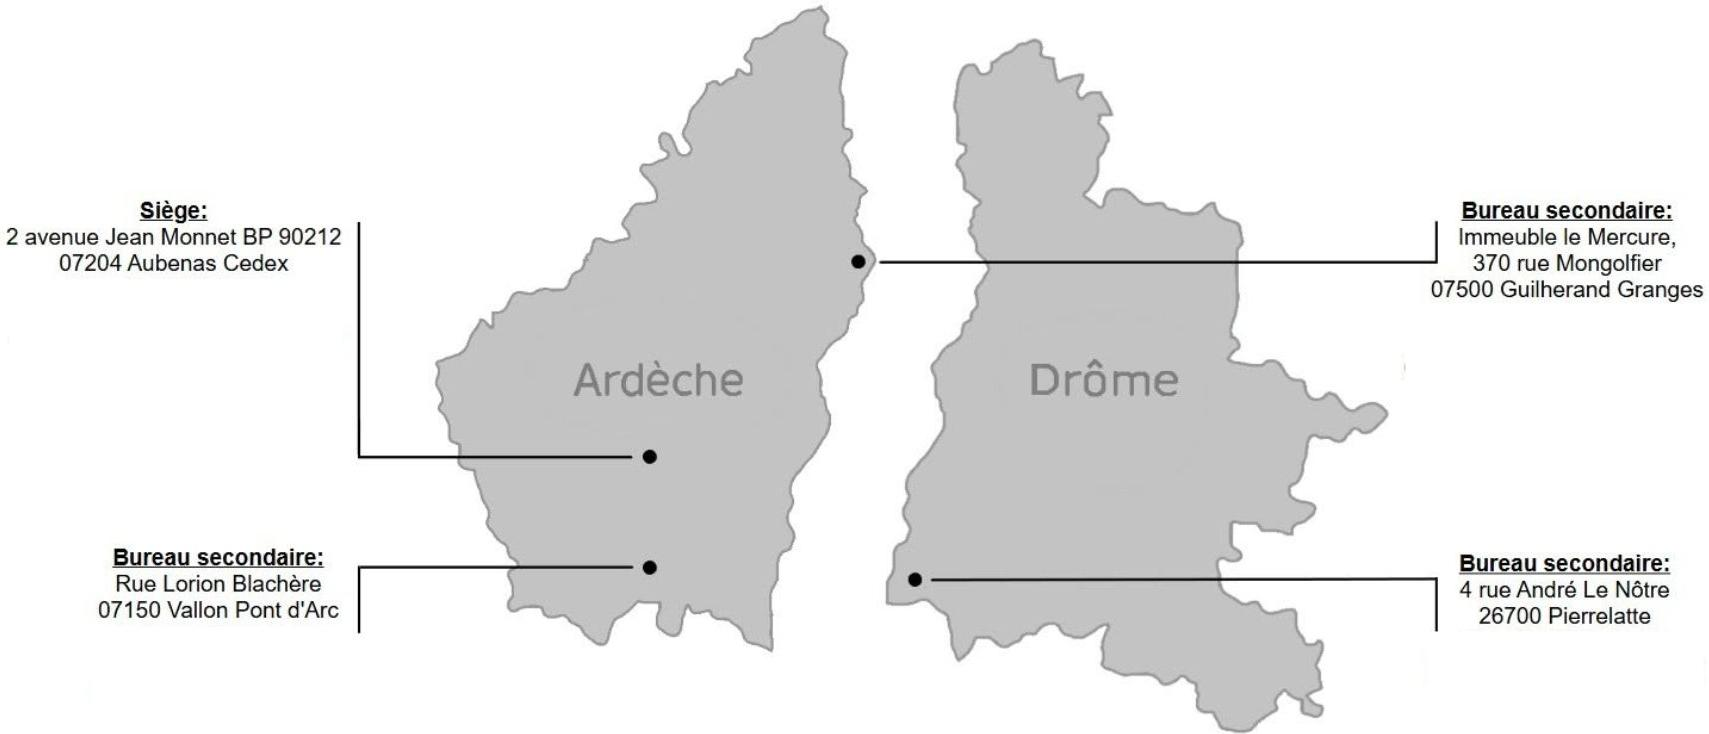
\includegraphics[width=\textwidth]{img/bureau_cropped.jpg}
  \caption{Implantation territoriale de GEO-SIAPP. La présence de quatre agences permet de répondre aux contraintes géographiques du département et explique la décentralisation des fonds d'archives. (Source~: \url{https://www.geo-siapp.com/index.php})}
  \label{fig:carte_agences}
\end{figure}

Ce projet de fin d'études s'est déroulé au sein du cabinet sur une période de six mois, de février à juillet 2026. La mission confiée consistait à concevoir et développer de bout en bout un outil informatique de traitement automatisé de ces archives, en vue de leur versement sur Géofoncier, le portail informatique national de la profession.

\subsection{Le cadre réglementaire et professionnel}

La profession de géomètre-expert est strictement réglementée, tout comme la gestion de la donnée foncière qu'elle produit et dont elle dispose du monopole légal en matière de fixation des limites de propriétés (loi du 7 mai 1946 \citep{loi_1946_geometre}). Le décret n°96-478 du 31 mai 1996 précise les obligations de la profession : seul le géomètre-expert est habilité à dresser les documents topographiques servant à la définition des droits fonciers \citep{decret_1996_geometre}. Par conséquent, chaque acte signé par le professionnel possède une valeur juridique opposable aux tiers et peut être produit en justice à tout instant.

En vertu de l'article 55 de ce même décret, le géomètre-expert a l'obligation de conserver ses archives et documents d'arpentage pendant une durée minimale de trente ans \citep{decret_1996_geometre}. Fait notable, cette obligation de conservation survit à l'arrêt de l'activité du cabinet : les archives doivent être transmises à un autre professionnel  en exercice ou, à défaut, remises au Conseil régional de l'Ordre. C'est précisément pour répondre à cette exigence que GEO-SIAPP s'est retrouvé dépositaire de fonds d'archives anciens, parfois dégradés par le temps, à l'issue de ses différentes opérations de rachat ou d'expansion dans la région.

À l'échelle nationale, l'Ordre des géomètres-experts a mis en place et entretient le portail Géofoncier. Cette plateforme centralise l'ensemble des interventions foncières réalisées sur le territoire national sous la forme de dossiers géolocalisées, facilitant ainsi les recherches \citep{geofoncier_portal}. Depuis 2021, une vaste opération nommée GEODEMAT, conduite conjointement avec la Direction Générale des Finances Publiques (DGFiP), ambitionne de numériser les documents cadastraux historiques (DMPC) déposés aux services fiscaux depuis 1956 \citep{geodemat_2021}. Néanmoins, cette initiative publique ne couvre pas les archives à caractère privé conservées par les cabinets (tels que les procès-verbaux de bornage, les registres manuscrits ou les croquis de terrain). La gestion, l'indexation et la remontée de ces informations  sur le portail demeurent sous la seule et entière responsabilité des géomètres-experts.

\subsection{Contexte du projet}

L'article 646 du Code civil stipule que \enquote{tout propriétaire peut obliger son voisin au bornage de leurs propriétés contiguës}. Cependant, l'exercice de ce droit est limité par le principe : \enquote{bornage sur bornage ne vaut}. En effet, la justice estime que si une limite de propriété a déjà été fixée de manière définitive par le passé (via un procès-verbal signé), il est juridiquement irrecevable d'exiger un nouveau bornage. Le géomètre n'est donc plus autorisé à redéfinir la limite : il a pour obligation de retrouver et de s'appuyer sur l'acte ancien pour la rétablir à son emplacement d'origine. C'est pour s'assurer du strict respect de cette règle que les directives de l'Ordre imposent au professionnel de procéder systématiquement à une \enquote{recherche d'antériorité}. 

Dans la pratique du cabinet, cela implique que la toute première étape d'une nouvelle mission consiste à interroger le portail Géofoncier. L'opérateur cherche à vérifier si une intervention a déjà eu lieu sur les parcelles concernées par le chantier, ou à proximité immédiate, afin de s'appuyer sur les actes juridiques existants. S'il s'agit d'une affaire récente, le plan numérisé peut souvent être téléchargé directement depuis la plateforme. En revanche, si l'opération est ancienne et n'a pas été versée numériquement, le géomètre doit solliciter par courriel le cabinet dépositaire du document. Cette démarche met en évidence la difficulté d'accès aux vieux plans : la recherche physique au sein des locaux d'archives est une tâche chronophage, souvent sans garantie quant au classement ou à la localisation exacte de la pièce. Conscients du temps consommé et non productif, et de la perte de rentabilité engendrée par ces recherches, certains cabinets vont même jusqu'à exiger une rémunération en contrepartie de la recherche et de la délivrance de ces plans.

Au sein de GEO-SIAPP, les archives non numériques couvrent la période de 1959 à 2007. Ce fonds est vaste et regroupe des documents très différents : des plans sur calque, des registres écrits à la main, ou encore d'anciens documents tapés à la machine. Certains de ces actes anciens apparaissent sur Géofoncier sous la forme d'une référence de DMPC, numérisée par la DGFiP dans le cadre de l'opération GEODEMAT : un professionnel peut ainsi constater qu'une intervention foncière a eu lieu sur une parcelle donnée. Mais cette trace ne donne pas accès aux pièces du dossier (plans, procès-verbaux, croquis, etc.) qui restent conservées physiquement, soit dans les locaux du cabinet dépositaire, soit aux archives du Centre des Impôts Fonciers compétent. Pour en obtenir copie, il faut les contacter directement.

Cette problématique d'accessibilité n'est pas un cas isolé. L'Ordre des géomètres-experts estime que plusieurs dizaines de millions de documents sont actuellement stockés dans les archives des cabinets français.

\subsection{Les défis techniques}

Le fonds à traiter couvre près de cinquante ans d'archives, ce qui se traduit par une diversité de documents : plans sur calque manuscrits, registres écrits à la main, actes dactylographiés, avec des mises en page sans standard. La difficulté principale n'est pas de traiter chaque type de document en particulier, mais de concevoir un programme unique capable de les aborder tous. Les anciens géomètres utilisaient des abréviations, l'écriture est manuscrite, et l'encre s'efface avec le temps. De plus, les documents sont parfois scannés de travers, tachés ou partiellement illisibles. Face à ces problèmes, les logiciels de reconnaissance de texte atteignent vite leurs limites et produisent trop d'erreurs pour que le résultat soit exploitable.

De plus, une contrainte s'impose : l'outil développé doit pouvoir être déployé et s'exécuter localement, sur l'unité centrale (CPU) d'une station de travail Windows du cabinet. Dans la mesure où les archives foncières contiennent des données à caractère personnel, assujetties au secret professionnel, tout traitement sur une infrastructure distante susceptible d'entraîner une fuite de données est exclu.

Ce mémoire s'articule donc autour de la problématique suivante : \textit{Dans quelle mesure est-il possible de concevoir un outil logiciel capable d'extraire avec fiabilité les données d'archives foncières très variées, tout en fonctionnant localement sur un ordinateur de bureau ?}

\subsection{Démarche employée}

L'objectif est alors de concevoir un outil capable d'extraire, depuis l'image scannée d'une archive, les informations exigées par l'API REST de Géofoncier (détaillé au chapitre~\ref{sec:analyse_metier}), à savoir le code INSEE de la commune, la localisation géographique de l'intervention, la date de l'acte au format ISO 8601 et le numéro de référence du dossier. Une fois ces informations renseignées, l'archive peut être géolocalisée sur la carte et versée sur le portail Géofoncier (chapitre~\ref{sec:integration}).

Pour répondre à cette problématique, la démarche s'articule autour de six étapes :

\begin{itemize}
    \item La classification : identification du type de document entrant pour savoir à quel endroit chercher les informations.
    \item Le prétraitement : nettoyage et redressement de l'image pour en optimiser la lisibilité.
    \item La segmentation spatiale : détection des zones utiles de l'image afin d'isoler les champs d'intérêt.
    \item L'extraction textuelle : transcription du contenu et extraction des entités pertinentes.
    \item Le contrôle et la validation : vérification de la cohérence des résultats extraits, suivie d'une validation par un opérateur humain. S'agissant d'actes fonciers officiels, cette vérification reste obligatoire.
    \item L'exportation : formatage des données validées et versement sur le portail Géofoncier.
\end{itemize}

Chaque étape est indépendante et peut être ajustée sans modifier les autres, ce qui facilite l'adaptation à un nouveau fonds d'archives.


\subsection{Organisation du mémoire}


Pour répondre à cette problématique et détailler la démarche adoptée au cours de ce projet, ce mémoire est structuré en huit chapitres principaux :

Le chapitre~\ref{sec:analyse_metier} analyse le contexte métier et le cadre juridique de la profession. Il caractérise le fonds d'archives de GEO-SIAPP, présente les contraintes de confidentialité qui imposent un traitement local, et détaille le fonctionnement du versement sur le portail Géofoncier.

Le chapitre~\ref{sec:etat_art} passe en revue les technologies existantes pour l'analyse automatique de documents : détection de zones, reconnaissance de texte imprimé et manuscrit, extraction d'entités, et modèles capables d'interpréter conjointement image et texte. Il justifie les choix retenus pour le projet.

Le chapitre~\ref{sec:architecture} présente l'architecture globale de la solution proposée. Il détaille chaque étape du traitement : classification des documents, prétraitement d'image, segmentation des zones d'intérêt, extraction du texte et identification automatique des informations pertinentes. Il décrit également la constitution du jeu de données d'entraînement et la gestion des cas d'erreur.

Le chapitre~\ref{sec:fiabilisation} est consacré à la fiabilisation des données extraites et à l'interface de contrôle mise à disposition des opérateurs. Il présente le formulaire de validation, le système de correction assistée et le module de recherche d'antériorités dans les registres numérisés.

Le chapitre~\ref{sec:integration} traite du versement des données sur le portail Géofoncier. Il décrit le calcul de la localisation géographique, l'envoi des documents et le mode d'exportation par lot. Il présente un cas d'étude réel et une évaluation quantitative des performances.

Le chapitre~\ref{sec:limites_perspectives} aborde les limites rencontrées, l'analyse des cas d'échec, et formule des pistes d'amélioration pour la suite du projet.

Enfin, le chapitre~\ref{sec:conclusion_generale} dresse le bilan des travaux réalisés, évalue les apports de la solution pour le cabinet GEO-SIAPP et présente le retour d'expérience personnel tiré de ce projet.





\clearpage
% !TeX root = main.tex

\section{Analyse du métier, de la donnée et des enjeux documentaires}
\label{sec:analyse_metier}

À la suite de la présentation des objectifs du projet (Chapitre~1), ce chapitre approfondit les contraintes propres à la situation du projet, justifiant les choix effectués par la suite car dépendant du lieu d'activité. Il précise la distinction entre le cadastre et les actes, explique le fonctionnement du versement sur Géofoncier via son API REST, caractérise les différents types d'archives, puis évoque la problématique de la filiation parcellaire. Enfin, il synthétise les contraintes de confidentialité et d'exécution locale.

\subsection{Cadastre et propriété foncière : distinction juridique}

Pour comprendre l'intérêt des archives, il est important de faire la différence entre le plan cadastral et les actes de bornage, l'interêt étant différent.

Créé en 1807 sous le régime de Napoléon I\textsuperscript{er}, le cadastre français avait à l'origine un objectif uniquement fiscal : recenser la totalité des propriétés foncières afin de récolter de façon équitable l'impôt foncier. Aujourd'hui, le Plan Cadastral Informatisé (PCI), géré et mis à jour par la Direction Générale des Finances Publiques (DGFiP), sert de fond de plan de référence pour l'aménagement du territoire.

Cependant, en droit français, le cadastre ne constitue ni un titre de propriété ni une délimitation juridique des terrains. La jurisprudence de la Cour de cassation rappelle que le cadastre ne fournit qu'une présomption fiscale et parcellaire. De plus, la précision du PCI est très variable : dans les zones rurales issues d'anciens plans napoléoniens vectorisés, les écarts de positionnement des limites cadastrales par rapport au terrain réel peuvent dépasser plusieurs mètres.


À l'inverse, la délimitation d'une propriété relève du monopole légal du géomètre-expert, réaffirmé par la loi n$^\circ$46-942 du 7 mai 1946 (\hyperref[ann:textes_loi]{voir Annexe~A -- [1]}). Conformément à l'article 646 du Code civil (\enquote{Tout propriétaire peut obliger son voisin au bornage de leurs propriétés contiguës}), la limite réelle entre deux terrains ne peut être fixée de manière définitive que par un PV de bornage. Rédigé par le géomètre-expert et signé par l'ensemble des propriétaires riverains, ce PV de bornage est un acte contradictoire ayant valeur juridique opposable aux tiers. Lors de cette opération, le géomètre matérialise les limites sur le terrain par des repères physiques (bornes OGE, clous d'arpentage) et les rattache au système officiel Lambert-93 avec une précision centimétrique.

Ainsi, alors que le cadastre ne propose qu'un découpage administratif et fiscal à valeur indicative, les archives conservées au sein des cabinets constituent la seule mémoire juridique de la propriété foncière.

Cette opposition entre le rôle fiscal du cadastre et le rôle juridique du géomètre-expert explique pourquoi la conservation des archives privées est importante pour les cabinets. Lorsqu'un litige survient entre des propriétaires riverains, les juges s'appuient en priorité sur les procès-verbaux de bornage et les plans d'arpentage anciens rédigés sur le terrain par le géomètre. Le plan cadastral n'est consulté qu'à titre subsidiaire. La disparition ou l'altération d'un dossier historique priverait le cabinet et les propriétaires des éléments de preuve nécessaires pour rétablir une limite de propriété.

\subsection{Le versement sur Géofoncier (API REST et Swagger)}

Les opérations foncières réalisées par les géomètres-experts font l'objet d'un versement sur le portail Géofoncier, créé par l'OGE en 2010. Ce versement répond à l'obligation de centraliser et de référencer toutes les interventions sur le territoire. Comme l'illustre la figure~\ref{fig:interface_geofoncier}, ce dernier affiche sous forme de pastilles la géolocalisation des opérations réalisées par l'ensemble de la profession (\hyperref[ann:textes_loi]{voir Annexe~A -- [4]}), ici pour une commune locale. Ce système permet aux cabinets de vérifier immédiatement si des travaux de bornage ou de division existent déjà sur une parcelle et de retrouver le géomètre qui a réalisé l'opération.

\begin{figure}[H]
  \centering
  \setlength{\fboxsep}{0pt}%
  \setlength{\fboxrule}{0.5pt}%
  \fbox{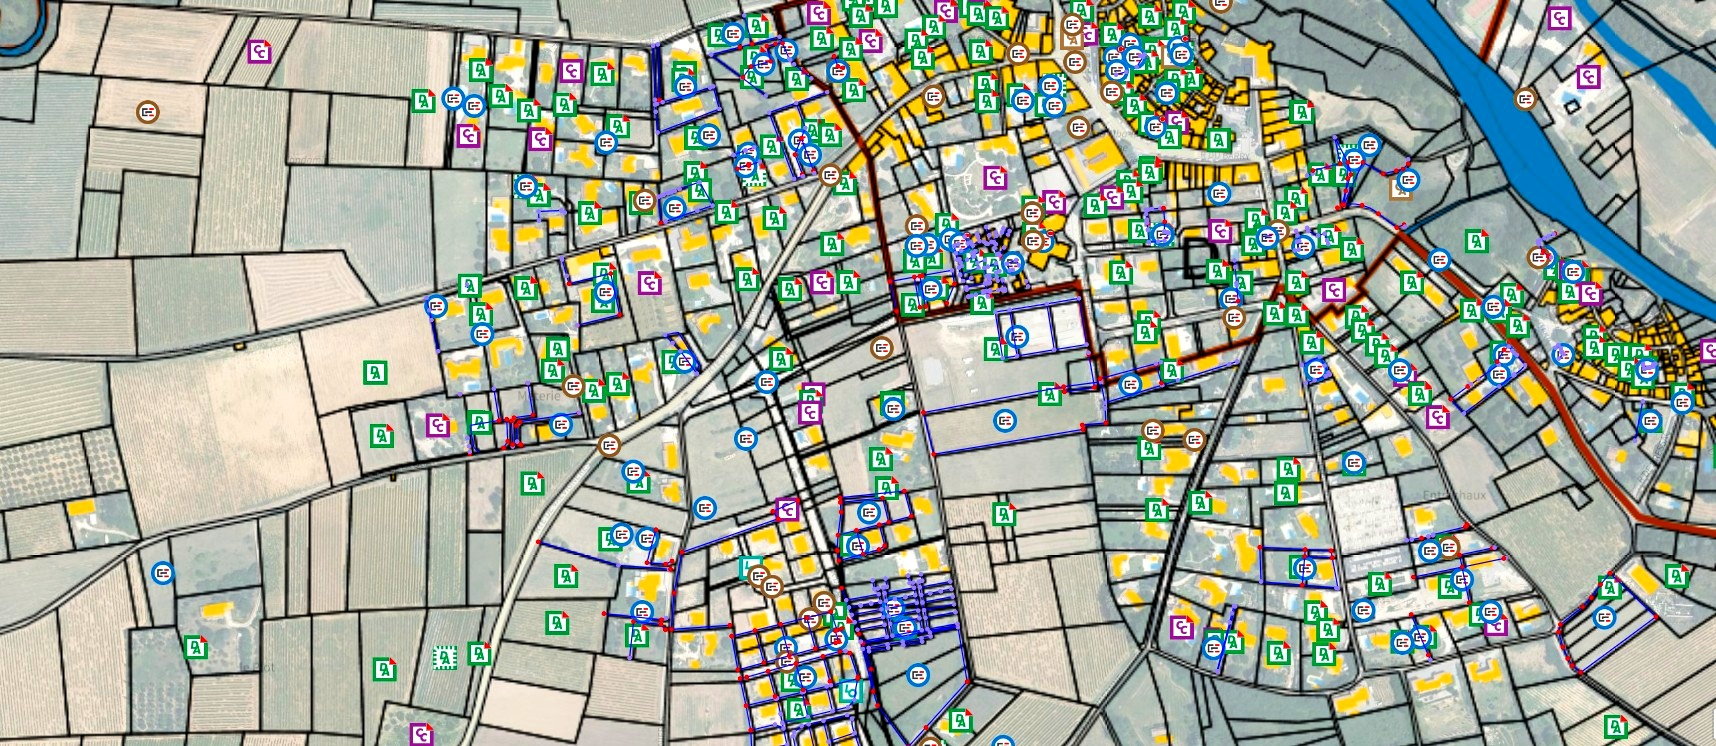
\includegraphics[width=0.85\textwidth]{img/Chap2_pastilles_enhanced.jpg}}\par
  \vspace{0.5em}
  \caption{Capture d'écran du portail GéofoncierEXPERT.}
  \label{fig:interface_geofoncier}
\end{figure}

Pour verser automatiquement des dossiers sans passer par une saisie manuelle sur le site web, l'OGE met à disposition une API REST (\hyperref[ann:textes_loi]{voir Annexe~A -- [5]}). L'ensemble des routes et des méthodes d'échange est documenté via une interface Swagger UI, qui permet de tester les requêtes et de consulter les formats attendus pour chaque composante (notamment `rfuoge` pour le RFU et `dossiersoge` pour la gestion des dossiers).

Le fonctionnement du versement repose sur plusieurs étapes. En principe, un serveur de préproduction est prévu pour tester les versements sans impacter la base réelle. Cependant, lors des travaux sur ce projet, le serveur de préproduction était indisponible et ne permettait pas de générer de jetons d'accès. Les développements et la constitution des requêtes ont donc été réalisés en s'appuyant directement sur les spécifications officielles de l'API.

L'accès aux services de l'API nécessite l'envoi d'un jeton d'authentification (Token) transmis dans l'en-tête HTTP de chaque requête, délivré après authentification des identifiants du géomètre-expert, et renouvelable toutes les 24 heures.

L'enregistrement d'une opération sur l'endpoint `rfuoge` nécessite de fournir une structure au format JSON contenant plusieurs informations obligatoires. Ces données comprennent le code INSEE à 5 chiffres de la commune (issu du Code Officiel Géographique \citep{insee_cog}), la date de l'acte au format ISO 8601 (`AAAA-MM-JJ`), le type d'acte selon le code OGE (par exemple `Bo` pour un bornage, `DA` pour un document d'arpentage), la référence interne du dossier au cabinet, ainsi que les coordonnées du centroïde ou l'emprise de l'opération en Lambert-93 (EPSG:2154). Un exemple de payload valide est présenté en figure~\ref{fig:payload_json_geofoncier}. L'objectif du projet est donc de concevoir une chaîne de traitement capable d'extraire automatiquement l'ensemble de ces éléments depuis les archives.



\begin{figure}[H]
  \centering

  \begin{verbatim}
  {
    "code_insee": "07019",
    "date_operation": "1984-05-12",
    "type_acte": "Bo",
    "reference_dossier": "GEO-1984-089",
    "geometry": {
      "type": "Point",
      "coordinates": [801452.35, 6391204.18]
    }
  \end{verbatim}
  \caption{Exemple de structure de données JSON transmise à l'API REST de Géofoncier pour enregistrer une opération (valeurs fictives).}
  \label{fig:payload_json_geofoncier}
\end{figure}

Lors de l'envoi, l'API renvoie un code de statut HTTP. Un code `201 Created` confirme la création de l'opération et le retour de l'identifiant Géofoncier. Si une donnée est mal formatée ou si le code INSEE n'existe pas, l'API retourne une erreur (`400 Bad Request` ou `422 Unprocessable Entity`).


\subsection{Structure des actes fonciers}

Le traitement automatisé vise spécifiquement les actes fonciers ayant une valeur juridique utiles au versement Géofoncier, à savoir les DMPC, les PV de bornage, ainsi que les registres d'affaires qui les répertorient, car sur ces derniers figurent des informations obligatoires sur les dossiers à verser.

Les DMPC sont établis lors des divisions parcellaires pour permettre la mise à jour du plan cadastral par la DGFiP. Rendus obligatoires en France depuis la réforme de la publicité foncière issue du décret n$^\circ$55-22 du 4 janvier 1955 et du décret n$^\circ$55-471 du 30 avril 1955, ces actes visent à garantir la concordance exacte entre les actes notariés publiés et la représentation cadastrale. Ces documents suivent un modèle Cerfa structuré, ce qui peut faciliter le repérage automatique des informations, étant à chaque feuille au même endroit. Ils comportent un cartouche (précisant la commune, la section et les numéros de parcelles) et un extrait de plan.

Les PV de bornage sont des actes sous seing privé qui fixent la délimitation réelle et définitive entre deux propriétés contiguës. Fondés sur l'article 646 du Code civil (issu du Code Napoléon de 1804) et sur le monopole légal réservé aux géomètres-experts, ces procès-verbaux possèdent une valeur juridique supérieure aux indications cadastrales comme évoqué précédement. Une fois signés de manière contradictoire par l'ensemble des propriétaires riverains, ils sont irrévocables, opposables aux tiers et lient définitivement les propriétaires actuels ainsi que leurs ayants droit. Contrairement aux DMPC, ne suivent pas de format standardisé. Le géomètre y détaille la désignation des biens, la liste des riverains présents, les repères physiques posés (bornes OGE, clous) et l'historique de la propriété. La disposition du texte, des signatures et la présence de croquis annexés varient selon les époques et les habitudes du géomètre rédacteur, bien qu'un ensemble d'informations obligatoires soit commun à chacun d'eux.

Outre ces actes, les registres du cabinet centralisent l'ensemble des affaires réalisées au fil des années. Ils constituent une source pour le traitement automatisé, car chaque ligne récapitule un certain nombre d'éléments d'un dossier (pouvant être le numéro d'affaire, date, nom du client, commune, références parcellaires), variant en fonction du registre.

En revanche, les pièces de travail à usage interne au cabinet, telles que les croquis de terrain bruts ou les carnets d'observations rédigés lors des mesures, ne sont pas destinées au versement sur Géofoncier et restent en dehors du périmètre d'extraction du projet.

\subsection{Le fonds d'archives du cabinet}

La mise en place du traitement nécessite d'analyser la composition du fonds d'archives conservé par le cabinet, qui rassemble environ 40~000 dossiers d'affaires créés depuis 1959. Le projet se concentre spécifiquement sur les archives stockées au siège d'Aubenas. D'autres fonds sont conservés dans les agences secondaires, comme à Vallon-Pont-d'Arc, ou appartiennent à des prédécesseurs de moindre taille qui ne sont pas visés par cette étude.

Comme l'illustre la figure~\ref{fig:repartition_archives}, le périmètre retenu se divise en cinq fonds principaux totalisant environ 23~600 dossiers. Les deux plus grands représentent 6~600 dossiers (28,0\,\%) et 6~000 dossiers (25,4\,\%), suivis par trois autres fonds de 4~500 dossiers (19,1\,\%), 3~500 dossiers (14,8\,\%) et 3~000 dossiers (12,7\,\%).

\begin{figure}[H]
  \centering
  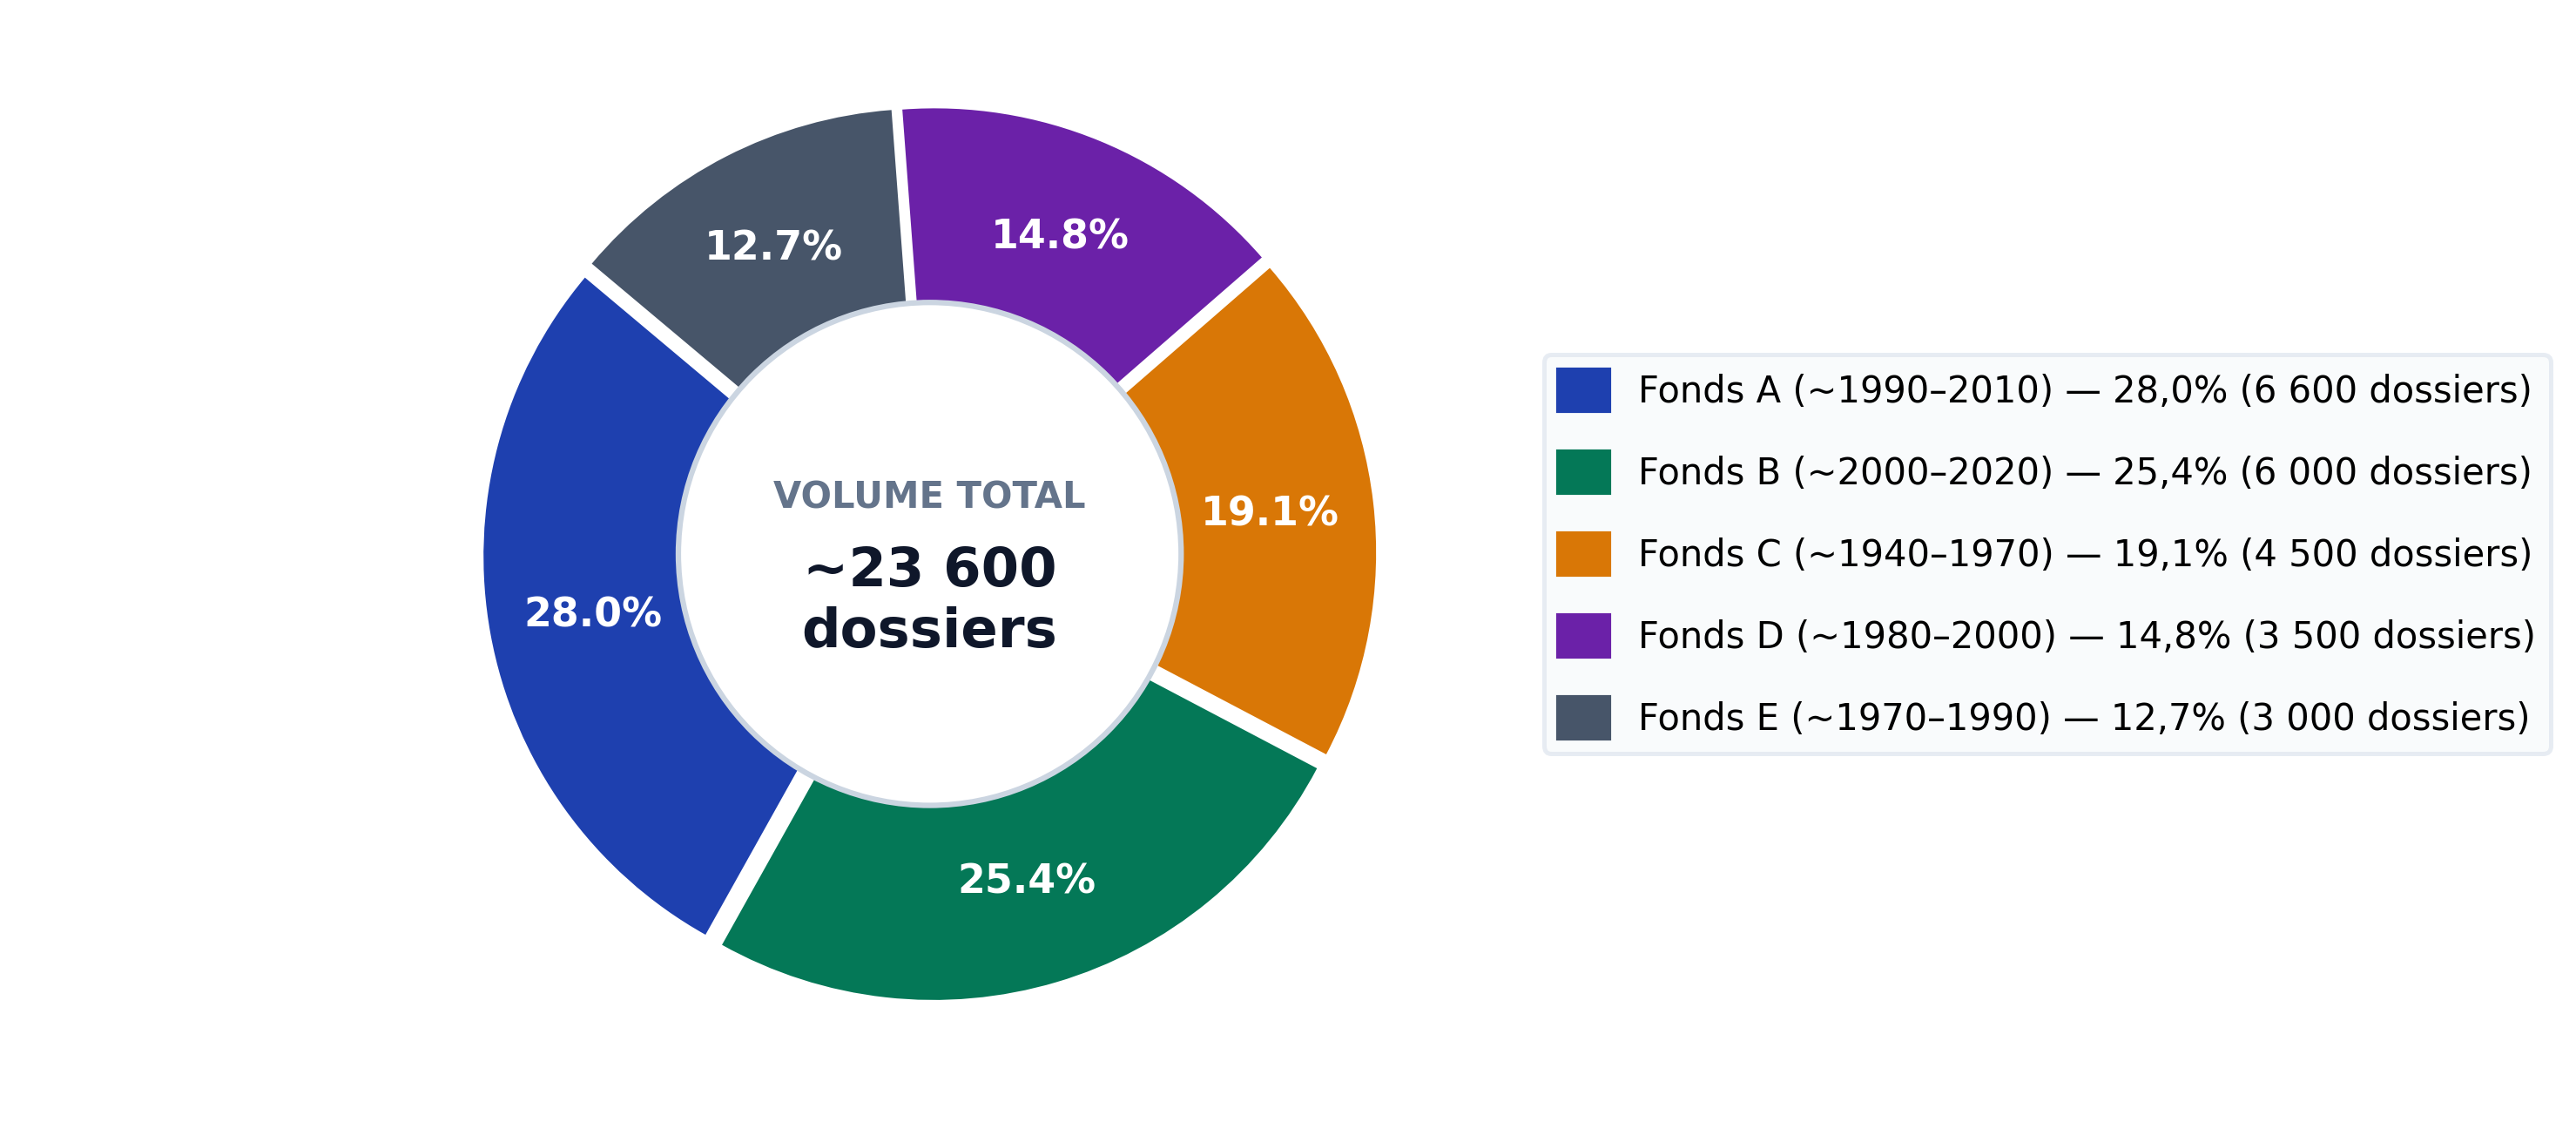
\includegraphics[width=0.95\textwidth]{img/repartition_archives.png}
  \caption{Répartition estimée du fonds d'archives du cabinet par fonds de géomètres prédécesseurs (Volume total : environ 23~600 dossiers).}
  \label{fig:repartition_archives}
\end{figure}

Chaque dossier contient l'ensemble des pièces d'une affaire : les actes fonciers (DMPC d'époque, PV et plans de bornage), les documents administratifs (devis, factures, courriers) et les notes de mesures terrain.

Pour le traitement automatique, on distingue trois grandes catégories de documents :

Les registres d'affaires tenus par chaque géomètre récapitulent la liste des dossiers. Pour les plus anciens rédigés à la main, la faible qualité du contraste et l'absence de grille fixe selon le prédécesseur rendent la lecture difficile.

Les documents dactylographiés (principalement entre 1980 et 2000) ont été créés à la machine à écrire. Le bruit présent dans le document (taches, ratures, etc.) nécessite un prétraitement pour améliorer la lisibilité.

Enfin, les dossiers contiennent de nombreuses pièces annexes (devis, factures). Le projet doit savoir trier les pages pour extraire uniquement les données des actes et des registres utiles.



La recherche d'informations au sein de ces fonds d'archives nécessite de croiser les pièces d'un même dossier. L'intérêt du traitement des registres repose sur ce recoupement des données. En effet, un document comme un DMPC ne comporte pas toutes les informations nécessaires, comme le numéro de dossier interne du cabinet. En revanche, les anciens géomètres inscrivaient sur une ligne de leur répertoire la date, le numéro d'affaire, le nom du client, la commune et les parcelles concernées parfois. La structure de cette ligne dépend toutefois du géomètre d'époque qui l'a rédigée. L'objectif est donc de faire correspondre chaque ligne du registre avec le plan ou le DMPC associé pour reconstituer le dossier complet.

\subsection{Analyse des registres et des difficultés de lecture}

Ces registres ne se présentent pas tous de la même façon : chaque géomètre avait sa propre tenue, les informations disponibles varient selon le fonds, et certains champs peuvent être absents d'un registre à l'autre. Certains traçaient des colonnes fixes, d'autres rédigeaient en texte continu ou utilisaient des imprimés différents.

Cette diversité entraîne trois difficultés principales pour le projet:

Premièrement, l'absence de grille pour certains registres rend l'alignement des colonnes variable d'un à l'autre et parfois d'une page à l'autre.

Deuxièmement, l'utilisation de guillemets de répétition (\enquote{"}), d'abréviations, ou encore de la mention \enquote{Idem} pour éviter de réécrire la commune ou la date d'une ligne sur l'autre. Le projet doit savoir conserver la valeur précédente en mémoire pour reconstituer ce type de schéma.

Troisièmement, le chevauchement de l'écriture manuscrite. Comme le montre la figure~\ref{fig:registre_ancien}, certaines lettres dépassent souvent sur les lignes du dessus ou du dessous, ce qui complique la séparation des lignes de texte par cases.

\begin{figure}[H]
  \centering
  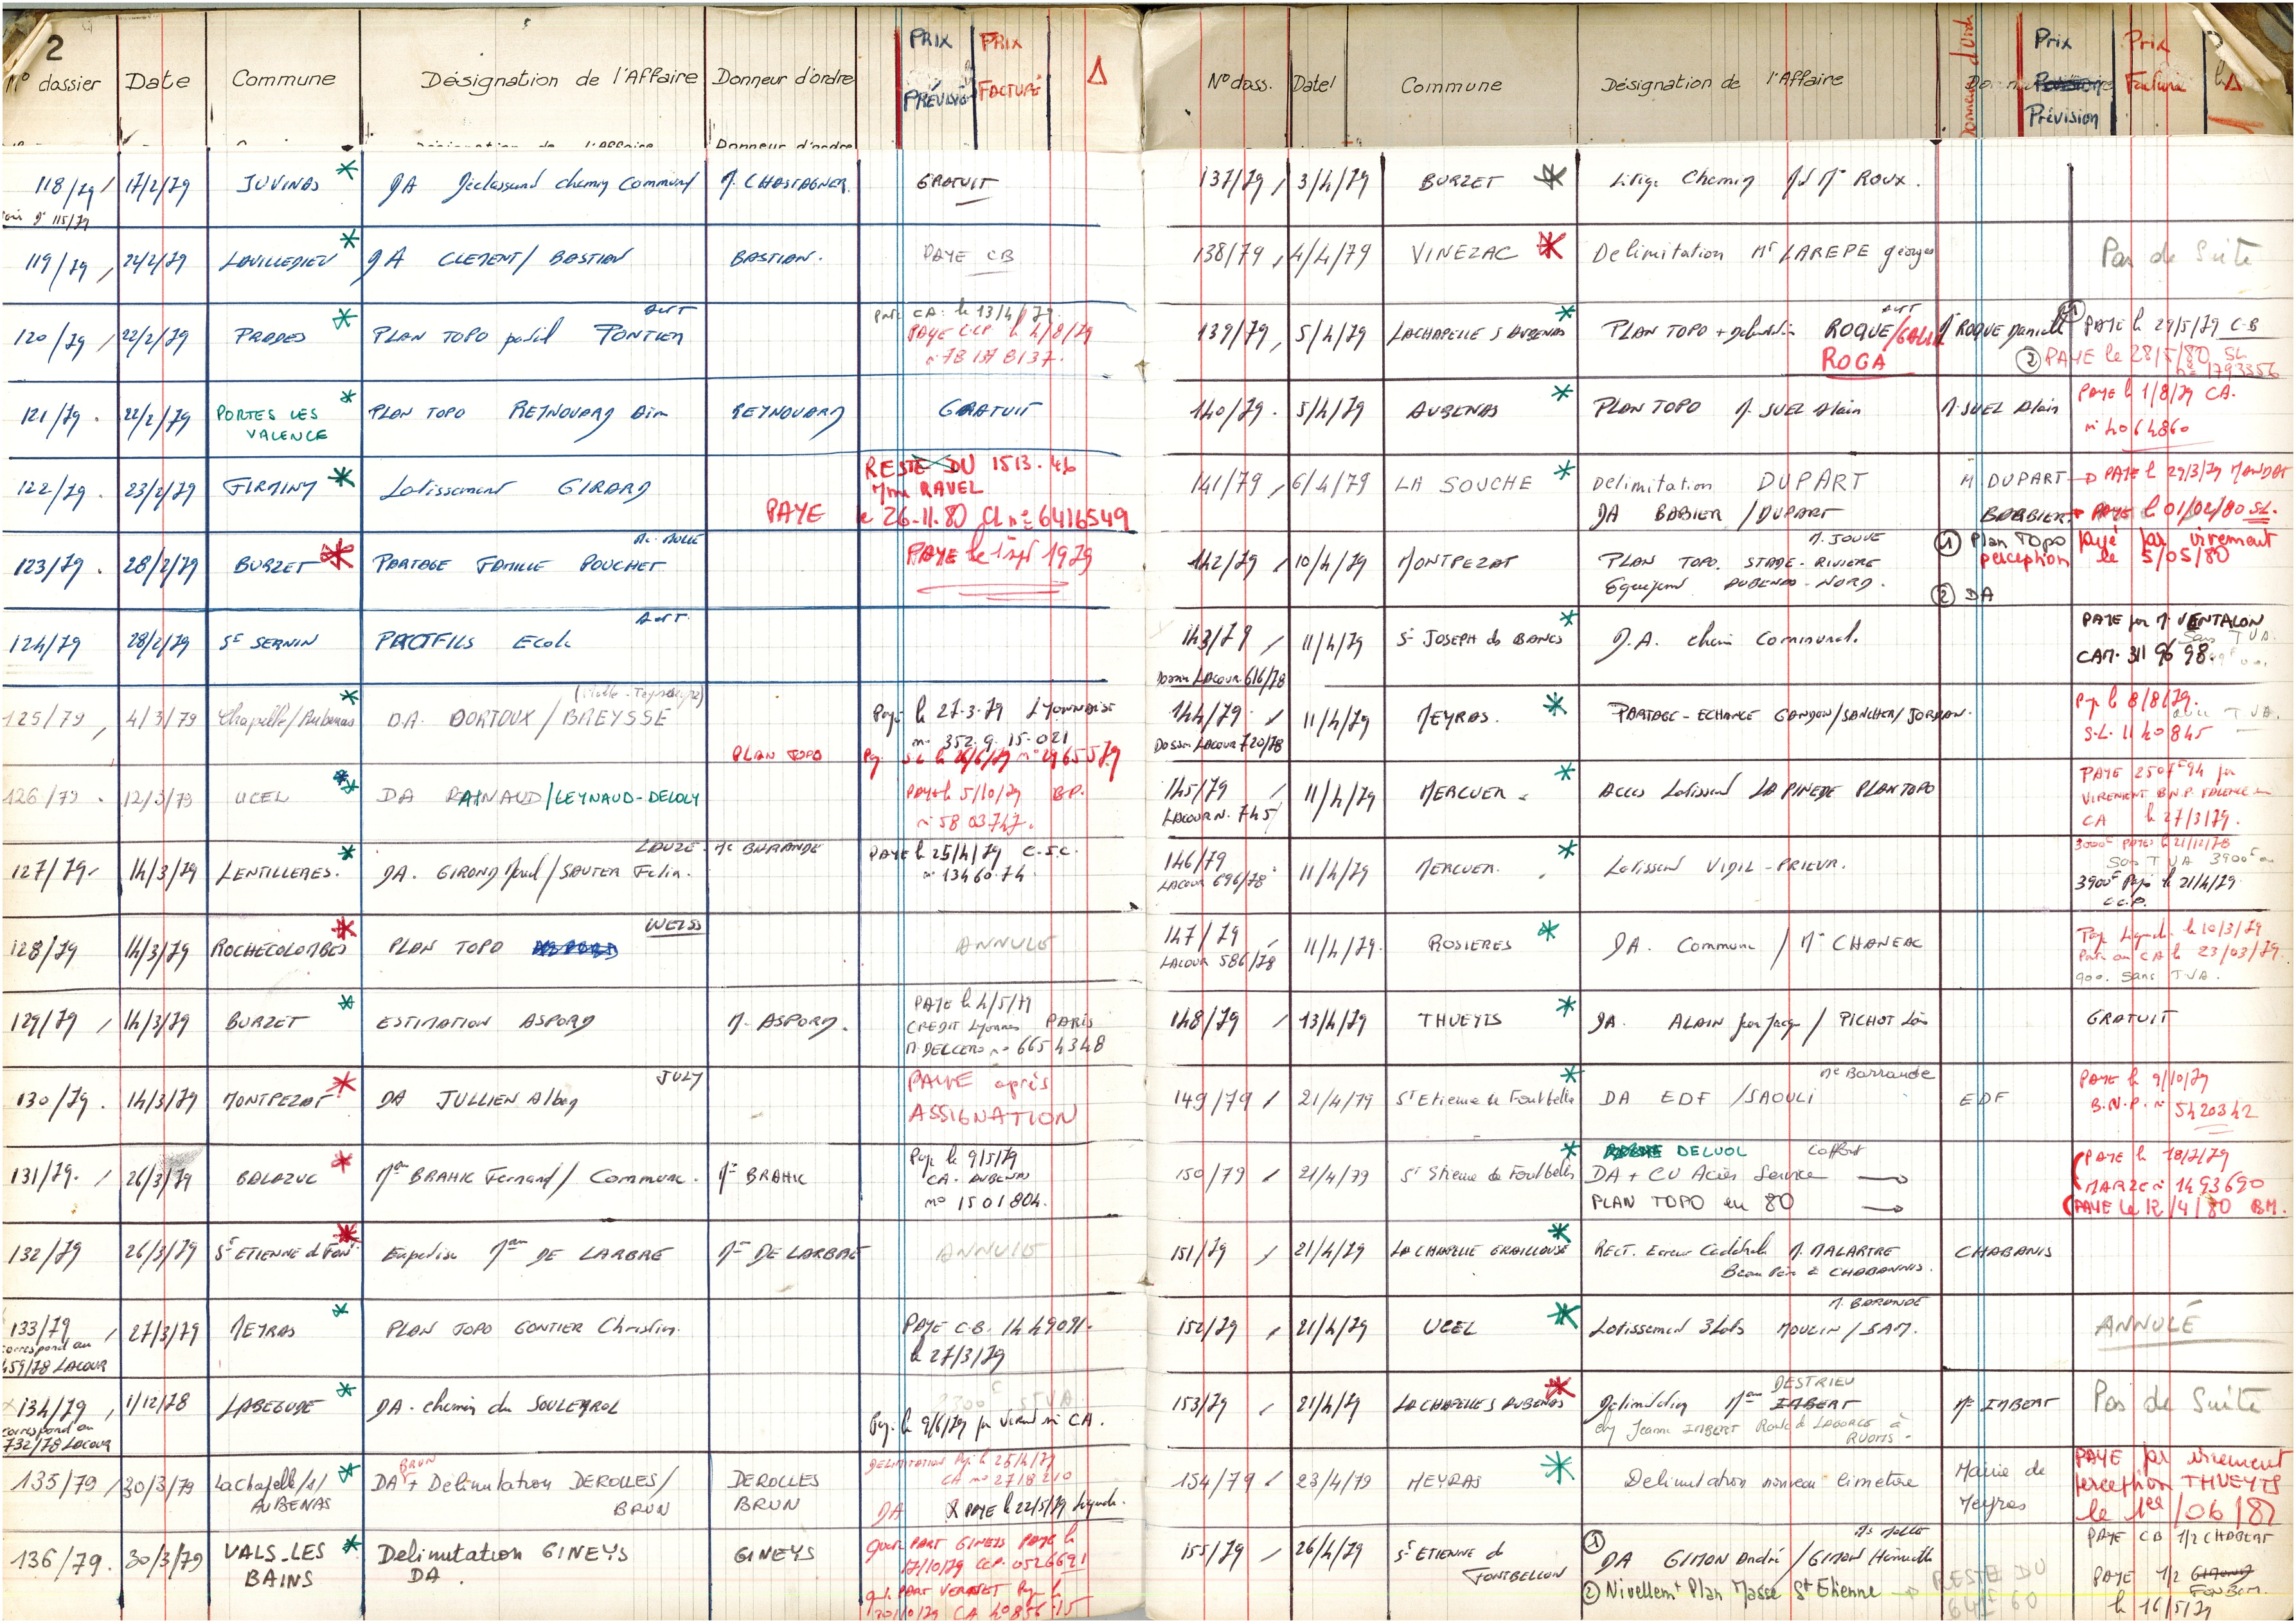
\includegraphics[width=\textwidth]{img/registre_manuscrit.jpg}
  \caption{Extrait d'un registre historique manuscrit du cabinet, illustrant l'écriture manuelle et les abréviations.}
  \label{fig:registre_ancien}
\end{figure}


La figure~\ref{fig:registre_ancien} illustre concrètement ces difficultés. On y observe deux pages d'un même registre  : la couleur de l'encre varie du noir au bleu, avec des annotations en rouge ajoutées après coup. Les colonnes sont tracées à la règle mais l'écriture déborde régulièrement d'une ligne sur l'autre. Certaines cases contiennent des abréviations, des renvois ou des symboles de répétition, tandis que d'autres sont laissées vides. La densité et le style de l'écriture changent visiblement d'un rédacteur à l'autre, parfois au sein d'une même page. On peut y distinguer les entêtes de numéro de dossier, date, commune, désignation de l'affaire, et donneur d'ordre. Ce registre couvre donc une partie des champs exigés par l'API Géofoncier : le numéro de dossier, la date et la commune sont présents. En revanche, les coordonnées géographiques de l'opération en Lambert-93 sont totalement absentes et doivent être extraites depuis le plan associé au dossier, tout comme le numéro de parcelle ainsi que de section.


Ainsi, la lecture des registres nécessite de traiter ces difficultés de présentation pour extraire correctement les données. Cependant, une fois ces informations récupérées, une autre étape est indispensable : réussir à lier les anciens numéros de parcelles aux références actuelles, qui ont pour la plupart évolué au fil des années.


\subsection{La filiation parcellaire}

La filiation parcellaire est importante pour retrouver les parcelles concernées par les archives du cabinet. Lorsqu'un géomètre recherche un dossier aujourd'hui, il dispose souvent uniquement du numéro de la parcelle actuelle. Cette même logique est à appliquer lors de la création de ces anciens dossiers. Les actes anciens ont été enregistrés sous les numéros parcellaires qui pour la plupart ont subi une modification, un découpage, ou tout autre intervention. L'un des objectif de ce projet est donc de retrouver les numéros de parcelles d'époques et de trouver une correspondance actuelle.

Lors d'une division foncière réalisée par un DMPC, l'ancien numéro de parcelle (la parcelle mère, par exemple \texttt{A 14}) est supprimé du cadastre et remplacé par de nouveaux numéros (les parcelles filles, par exemple \texttt{A 115} et \texttt{A 116}). Au fil du temps, ces nouvelles parcelles peuvent elles aussi être divisées. Sans le suivi de ces changements successifs, une recherche effectuée sur la parcelle actuelle ne permet de retrouver aucune localisation, le portail Géofoncier étant mis à jour régulièrement.

\begin{figure}[H]
  \centering
  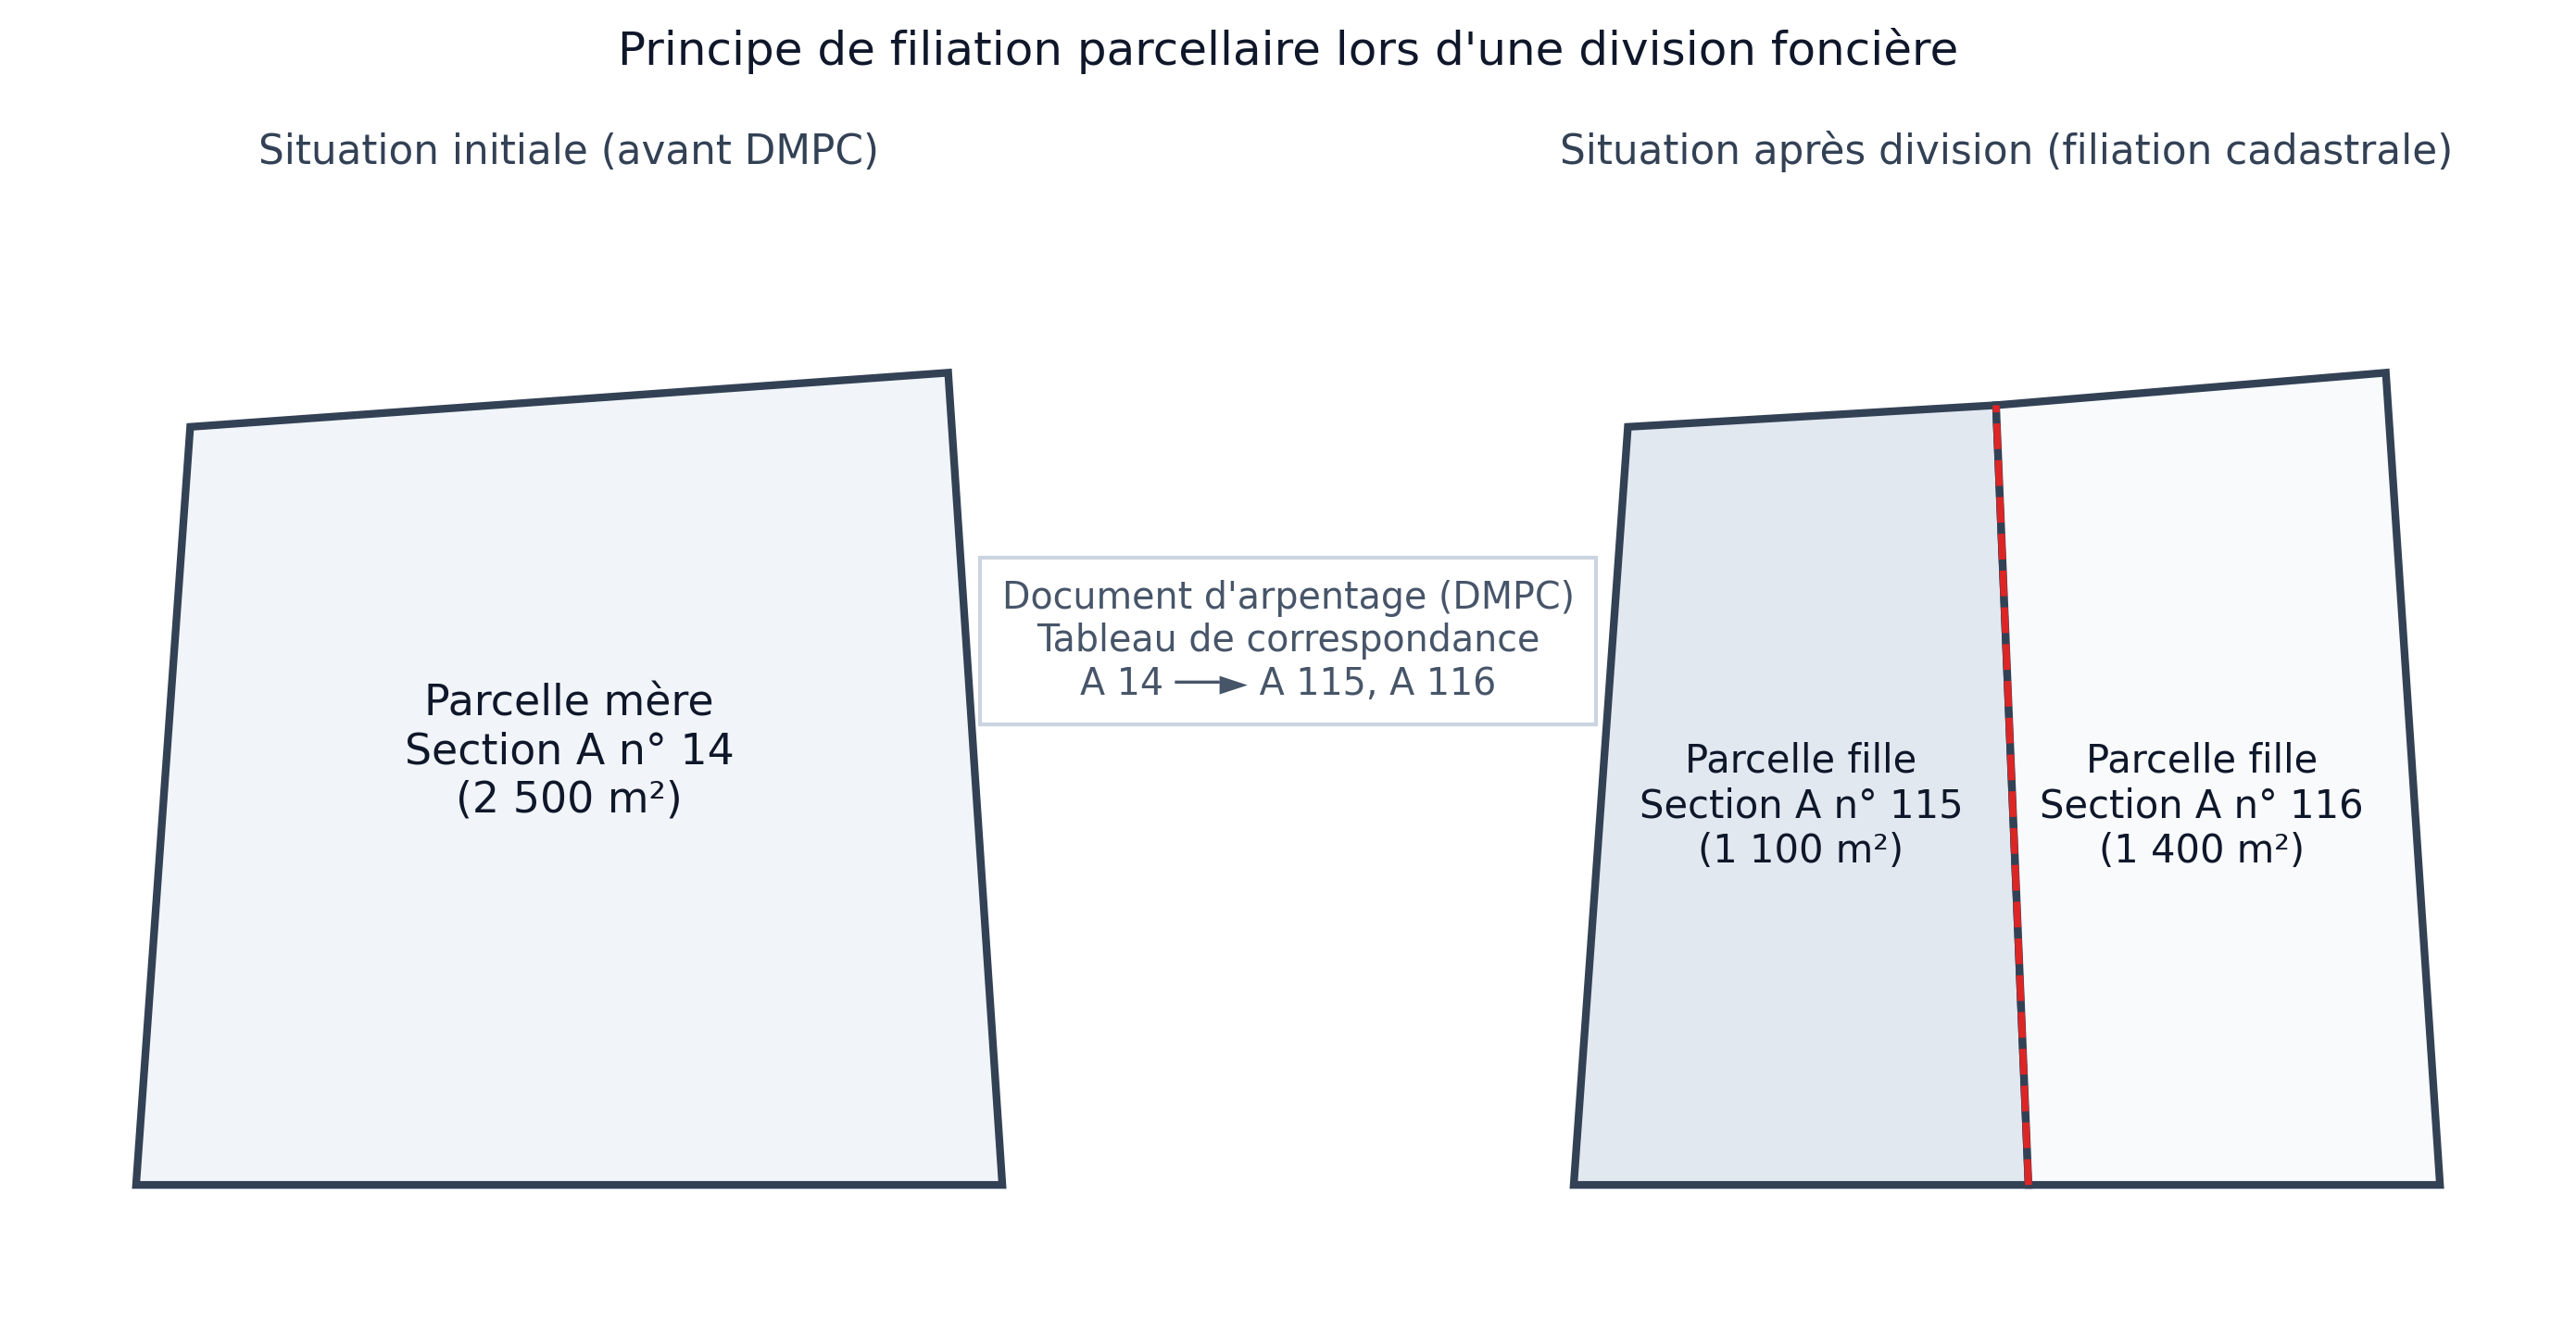
\includegraphics[width=0.95\textwidth]{img/filiation_parcellaire.png}
  \caption{Principe de filiation parcellaire lors d'un DMPC (remplacement de la parcelle mère A 14 par les parcelles filles A 115 et A 116).}
  \label{fig:filiation_parcellaire}
\end{figure}

Cette filiation est tenue à jour par la DGFiP à chaque validation d'un nouveau DMPC. Elle est enregistrée dans la matrice cadastrale et directement accessible aux géomètres sur le portail Géofoncier ainsi que par son API. Concrètement, cette base conserve l'historique des modifications sous forme d'associations entre chaque parcelle supprimée (la mère) et les parcelles créées (les filles).

En interrogeant cette base de filiation, le projet peut remonter automatiquement la chaîne des parcelles mères successives. Cela permet d'associer une parcelle contemporaine recherchée par le géomètre au numéro d'origine inscrit dans l'acte d'époque, et ainsi de retrouver le dossier correspondant. Pour ce projet, la base de données est téléchargeable sur le site de la DGFiP, et découpé par département. seul les modifications pour le département de l'Ardèche a été retenu. 


\subsection{Les contraintes de numérisation}

La réussite de l'extraction automatique dépend directement de la qualité des documents papier et des choix faits lors de leur numérisation au cabinet. Les archives conservées présentent en effet plusieurs types de détériorations physiques.

Avec le temps, le papier et les calques vieillissent et jaunissent, ce qui réduit le contraste entre l'encre et le fond. Sur les calques transparents, l'écriture du verso transparaît souvent au scanner et se mélange au texte du recto. De plus, la manipulation des dossiers au fil des années a laissé des plis et des déchirures. Il n'est pas rare non plus de trouver des annotations ajoutées après coup au crayon ou au stylo par les géomètres, qui viennent surcharger le document d'origine.

Sur les DMPC en particulier, les tampons officiels de réception posés par le cadastre (souvent avec une encre rouge ou bleue) recouvrent fréquemment le cartouche et masquent une partie des numéros de parcelles.

Toutes ces contraintes imposent de régler soigneusement les paramètres de numérisation selon le type de pièce, afin de conserver la meilleure lisibilité possible (tableau~\ref{tab:param_numerisation}).


\begin{table}[H]
  \centering
  \caption{Paramètres de numérisation retenus selon la nature des pièces d'archives.}
  \label{tab:param_numerisation}
  \small
  \begin{tabular}{p{4.5cm} c c c}
    \toprule
    \textbf{Type de document} & \textbf{Résolution (DPI)} & \textbf{Mode couleur} & \textbf{Format de fichier} \\
    \midrule
    Registres manuscrits  & 300 DPI & Niveaux de gris & PDF / TIFF  \\
    Formulaires DMPC et DA & 300 DPI & Couleur (24 bits) & PDF  \\
    PV de bornage et actes & 300 DPI & Niveaux de gris & PDF  \\
    Plans grand format (A3/A2) & 200 DPI & Couleur (24 bits) & PDF / JPEG \\
    Pièces annexes (factures) & 200 DPI & Noir et blanc & PDF  \\
    \bottomrule
  \end{tabular}
\end{table}

Le mode couleur est indispensable pour les formulaires comportant des tampons ou des traits de couleur, car il permet aux algorithmes de prétraitement de séparer les tampons de l'encre du texte, ou alors de comprendre quelles sont les anciennes ou les nouvelles parcelles.



\subsection{Synthèse des contraintes et des besoins du projet}


À la suite de cette analyse du métier, des archives et du fonctionnement de l'API, plusieurs contraintes et besoins ressortent pour le projet :

Tout d'abord, la conformité des données pour l'API exige de transmettre une structure JSON exacte respectant les formats attendus (code INSEE à 5 chiffres, date ISO 8601 et coordonnées en Lambert-93).

Ensuite, le tri des documents et le recoupement des informations imposent d'isoler les actes utiles (DMPC, PV de bornage) des pièces annexes (devis, factures) et de croiser les données des registres avec les pièces scannées pour compléter les informations manquantes.

De plus, la recherche par la filiation parcellaire doit s'appuyer sur l'historique des parcelles pour faire le lien entre les numéros d'époque figurant sur les archives et les numéros actuels recherchés.

Enfin, la confidentialité et l'exécution locale imposent que l'ensemble des traitements d'analyse d'image et d'extraction de texte s'effectue directement sur les postes du cabinet, sans envoyer de données sur des serveurs externes.

Ainsi, ces différentes exigences imposent de s'appuyer sur des solutions techniques capables de traiter aussi bien des documents imprimés que des registres manuscrits. Le chapitre suivant présente l'état de l'art des technologies d'extraction et d'analyse documentaire afin de sélectionner les outils les plus adaptés aux besoins du cabinet.

\clearpage
% !TeX root = main.tex

\section{État de l'art}
\label{sec:etat_art}

Ce chapitre passe en revue les technologies disponibles pour l'analyse automatique de documents. Pour chaque méthode, le fonctionnement, les résultats et les limites sont analysés afin de justifier les choix retenus pour la chaîne de traitement.

\subsection{La lecture de texte imprimé (OCR)}
\label{subsec:ocr}

La reconnaissance optique de caractères (OCR - \textit{Optical Character Recognition}) a été conçue pour automatiser la lecture de documents imprimés ou dactylographiés. L'objectif est de transformer une image de texte en caractères numériques exploitables par un ordinateur.

Le fonctionnement classique repose sur le découpage successif des éléments du document. L'image est d'abord binarisée pour séparer l'encre du papier. Le moteur repère ensuite les lignes de texte, puis découpe chaque ligne en mots et chaque mot en caractères isolés. Enfin, chaque caractère découpé est comparé à des modèles connus pour être identifié. Le moteur Tesseract illustre bien ce principe : pour repérer la ligne de base du texte même si la page est penchée ou courbée (comme près de la reliure d'un livre numérisé), il trace une ligne courbe mathématique (une spline quadratique) qui épouse l'ondulation des mots. Cela lui permet de lire le texte sans devoir redresser ou déformer l'image au préalable \citep{smith_tesseract_2007}.

Avec l'arrivée du deep learning, l'OCR n'a plus besoin de découper chaque caractère un par un. Les modèles modernes lisent la ligne entière d'un seul coup \citep{shi_crnn_2015}. \cite{baek_stract_2019} décomposent ce fonctionnement en quatre étapes principales, illustrées par la Figure~\ref{fig:ocr_pipeline} :

\begin{itemize}
  \item \textbf{La transformation géométrique (Trans.)} : normaliser la forme de la ligne de texte pour corriger les angles ou les déformations.
  \item \textbf{L'extraction de caractéristiques (Feat.)} : analyser les formes visuelles de l'image à l'aide d'un réseau de convolution (CNN).
  \item \textbf{La modélisation de séquence (Seq.)} : prendre en compte le contexte entre les lettres grâce à un réseau récurrent (BiLSTM).
  \item \textbf{La prédiction (Pred.)} : convertir la séquence visuelle en texte final grâce à une fonction d'alignement (CTC) ou d'attention.
\end{itemize}

\begin{figure}[H]
    \centering
    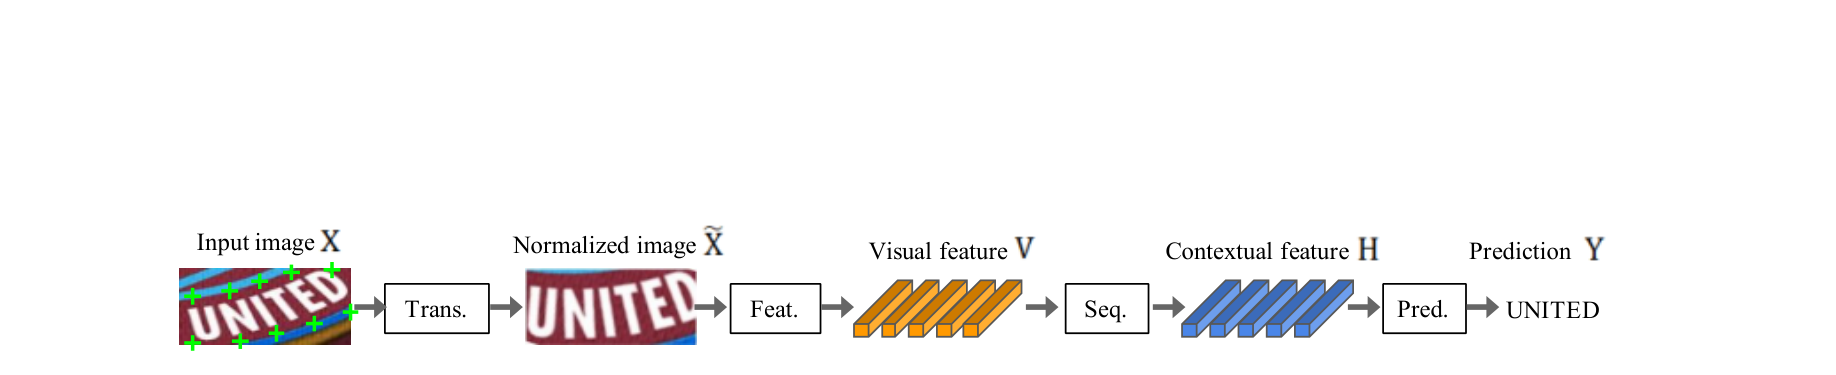
\includegraphics[width=\textwidth]{img/baek_ocr_pipeline_crop.png}
    \caption{Chaîne de reconnaissance de texte imprimé en quatre étapes : transformation géométrique (Trans.), extraction de caractéristiques visuelles (Feat.), modélisation de séquence (Seq.) et prédiction du texte (Pred.). Extrait de \cite{baek_stract_2019}.}
    \label{fig:ocr_pipeline}
\end{figure}

Cette méthode est fiable sur du texte imprimé ou dactylographié. En revanche, elle trouve sa limite sur l'écriture manuscrite, car le chevauchement des lettres empêche le modèle de distinguer les caractères correctement, et donc de trouver une correspondance avec son entraînement.

Pour surmonter les dégradations physiques des papiers anciens, les moteurs de numérisation s'appuient souvent sur des filtres de binarisation adaptative. La méthode d'Otsu cherche un seuil global optimal en minimisant la variance intra-classe des intensités de gris, ce qui fonctionne bien sur un fond homogène. Néanmoins, lorsque le document présente des taches d'humidité ou un jaunissement inégal, la binarisation de Sauvola calcule un seuil local pour chaque pixel en fonction de la moyenne et de l'écart-type de son voisinage. Ce traitement local préserve les traits fins des caractères imprimés sans amplifier les ombres de fond ou le bruit du papier.



\subsection{La reconnaissance de l'écriture manuscrite (HTR)}
\label{subsec:htr}

La reconnaissance de texte manuscrit (HTR - \textit{Handwritten Text Recognition}) a été conçue pour lire l'écriture à la main, sur laquelle l'OCR échoue. En écriture manuscrite, les lettres sont attachées, déformées et de tailles variables. Tenter de séparer chaque caractère individuellement provoque des erreurs systématiques. Pour résoudre ce problème, les systèmes HTR ne découpent pas les lettres : ils analysent la ligne entière comme un signal visuel continu.

La Figure~\ref{fig:rem_workflow} détaille le fonctionnement général de cette approche en trois étapes \citep{chague_htr-united_nodate} :

\begin{itemize}
  \item \textbf{La segmentation en lignes} : le système repère l'emplacement exact de chaque ligne de texte dans la page. Il trace une ligne de base (\textit{baseline}) sous l'écriture et extrait le masque d'image correspondant à la ligne.
  \item \textbf{L'analyse de la mise en page} : le modèle détermine l'ordre logique de lecture des différents blocs ou segments extraits de la page.
  \item \textbf{La transcription} : chaque portion d'image de ligne est convertie directement en une chaîne de caractères.
\end{itemize}

\begin{figure}[H]
    \centering
    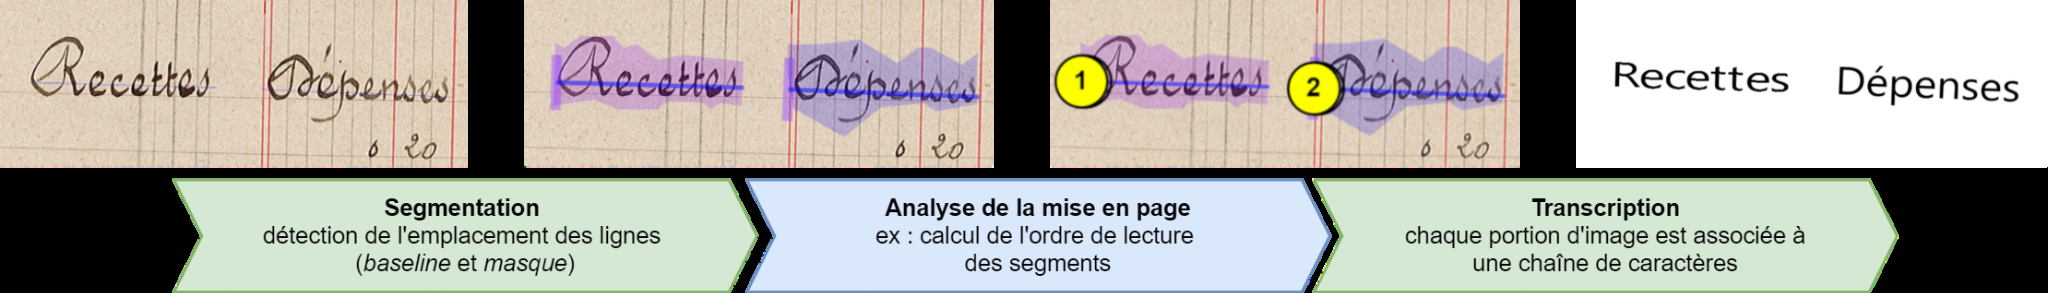
\includegraphics[width=\textwidth]{img/chague_fig1.png}
    \caption{Étapes de traitement d'un système HTR : segmentation de la page en lignes, analyse de la mise en page, puis transcription de chaque portion d'image en texte. Extrait de \cite{chague_htr-united_nodate}.}
    \label{fig:rem_workflow}
\end{figure}

Pour réaliser la phase de transcription, la littérature scientifique privilégie deux grandes architectures de réseaux de neurones.

La première repose sur l'alliance de réseaux de convolution et d'un alignement temporel (CNN + CTC), comme par exemple le modèle PyLaia \citep{tarride_improving_2024}. Des couches de convolution extraient d'abord la représentation visuelle de la ligne. Un réseau bidirectionnel (BLSTM) parcourt ensuite ces caractéristiques pour capter le contexte des mots. Enfin, la fonction de perte CTC (\textit{Connectionist Temporal Classification}) calcule la séquence de texte la plus probable sans imposer d'annoter la position exacte de chaque lettre dans l'image. Cette méthode présente l'avantage d'être légère en calcul et de bien s'entraîner sur des volumes restreints de données.

La seconde approche s'appuie sur l'architecture des Transformers, utilisée par le modèle TrOCR \citep{alkendi_advancements_2024}. L'image de la ligne est découpée en petits carrés visuels, appelés patchs. Un encodeur visuel (ViT) transforme ces patchs en vecteurs, qu'un décodeur de langage utilise pour générer le texte mot après mot. Le modèle calcule un poids visuel pour chaque région de l'image grâce au mécanisme d'attention issu de \cite{vaswani_attention_2017} et repris par \cite{alkendi_advancements_2024} :

\begin{equation}
  \text{Attention}(Q, K, V) = \text{softmax}\!\left(\frac{Q K^T}{\sqrt{d_k}}\right) V
\end{equation}

Dans cette formule, $Q$, $K$ et $V$ représentent les projections des patchs d'image sous forme de requêtes, de clés et de valeurs, et $d_k$ désigne la dimension des clés. Concrètement, le produit $Q K^T$ évalue la similitude entre le caractère recherché et chaque zone de l'image. La fonction \text{softmax} convertit ces scores en poids d'attention compris entre 0 et 1 : plus la correspondance entre la requête $Q$ et la clé $K$ est forte, plus le poids attribué à la valeur visuelle $V$ augmente. À chaque caractère généré, le réseau focalise ainsi son attention directement sur le tracé de la lettre correspondante. 
Sur des documents d'archives en français, ces modèles atteignent des taux d'erreur sur les caractères très faibles, inférieurs à 5~\% \citep{alkendi_advancements_2024, beatrice_challenges_2023}.

La principale contrainte du HTR est sa dépendance à la qualité du découpage des lignes. Si un tampon, une tache ou un élément de tableau vient couper le tracé d'une ligne, la phase de transcription perd en précision et génère des erreurs de lecture.

Pour bien comprendre la différence entre l'OCR et le HTR, présenté dans le chapitre précédent, elle repose sur le type de texte à lire et sur la façon dont le moteur l'analyse :

\begin{itemize}
  \item \textbf{L'OCR} s'applique au texte imprimé (\textit{Printed Text}). Comme les lettres sont régulières et séparées, le système cherche à isoler chaque caractère ou petit bloc avant de l'identifier.
  \item \textbf{Le HTR} s'applique à l'écriture manuscrite (\textit{Handwritten Text}). Comme les lettres sont attachées et varient selon les personnes, le système ne cherche pas à découper les caractères : il lit la ligne entière comme un tracé continu.
\end{itemize}

La Figure~\ref{fig:text_recognition_taxonomy} illustre cette séparation entre les technologies de reconnaissance de texte.

\begin{figure}[H]
    \centering
    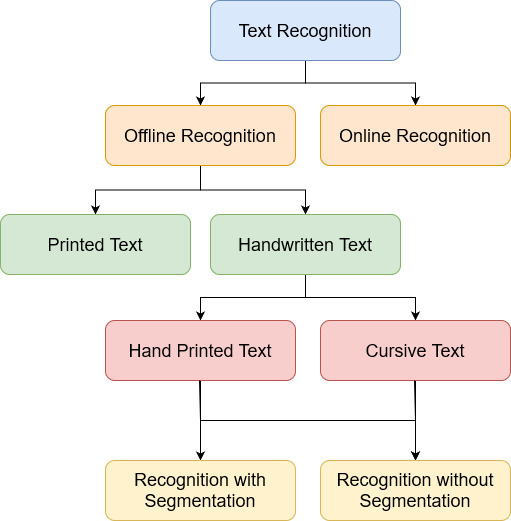
\includegraphics[width=0.55\textwidth]{img/fig_alkendi_p3_1.jpeg}
    \caption{Classification des systèmes de reconnaissance de texte : distinction entre le texte imprimé (\textit{Printed Text} / OCR) et le texte manuscrit (\textit{Handwritten Text} / HTR). Extrait de \cite{alkendi_advancements_2024}.}
    \label{fig:text_recognition_taxonomy}
\end{figure}

Cette arborescence résume la classification des systèmes de reconnaissance de texte. Elle sépare le traitement en deux branches : le traitement hors ligne sur des images scannées et le traitement en ligne en temps réel. Pour les images d'archives, la classification distingue le texte imprimé (OCR) et le texte manuscrit (HTR), qui nécessite une lecture globale sans découpage préalable des caractères.

Comme nous le verrons lors de la présentation de l'architecture (chapitre~\ref{sec:architecture}), le choix s'est porté sur une utilisation conjointe d'EasyOCR pour les parties imprimées et du modèle HTR PyLaia pour l'écriture manuscrite des anciens registres. PyLaia permet d'obtenir un compromis efficace entre rapidité d'exécution et autonomie locale, évitant ainsi d'alourdir les calculs sur les serveurs du cabinet.


Lorsque des documents associent texte imprimé et écriture manuscrite, des approches hybrides peuvent être envisagées.


\subsection{Les approches hybrides : OCR et HTR combinés}
\label{subsec:hybrid_ocr_htr}

En réalité, beaucoup de documents mélangent du texte imprimé et des ajouts écrits à la main, comme un formulaire pré-rempli. Un modèle OCR classique échoue sur les écritures manuscrites, tandis qu'un modèle HTR peut faire des erreurs sur du texte imprimé.

Pour résoudre ce problème, des approches hybrides ont été développées afin de traiter conjointement les deux types d'écriture. 

D'après la littérature scientifique, deux méthodes principales existent :

\begin{itemize}
  \item L'entraînement sur des exemples variés : le modèle TrOCR \citep{li_trocr_2021} s'appuie sur une architecture Transformer entraînée à la fois sur du texte imprimé et du texte écrit à la main. La Figure~\ref{fig:trocr_arch} montre ce principe : l'image de la ligne est découpée en petits carrés visuels (\textit{Image Patches}), convertis en vecteurs avec leur position, puis transmis à un encodeur visuel. Le décodeur produit ensuite le texte mot à mot. Comme le modèle a appris sur les deux formes d'écriture, il s'adapte tout seul sans étape de tri.
  \item La combinaison de deux outils successifs : des systèmes comme PaddleOCR \citep{du_ppocr_2020} ou EasyOCR utilisent un premier modèle pour repérer l'emplacement des lignes sur la page (comme DBNet \citep{liao_dbnet_2020}), puis un second modèle chargé uniquement de lire le texte présent dans ces zones.

\end{itemize}

\begin{figure}[H]
    \centering
    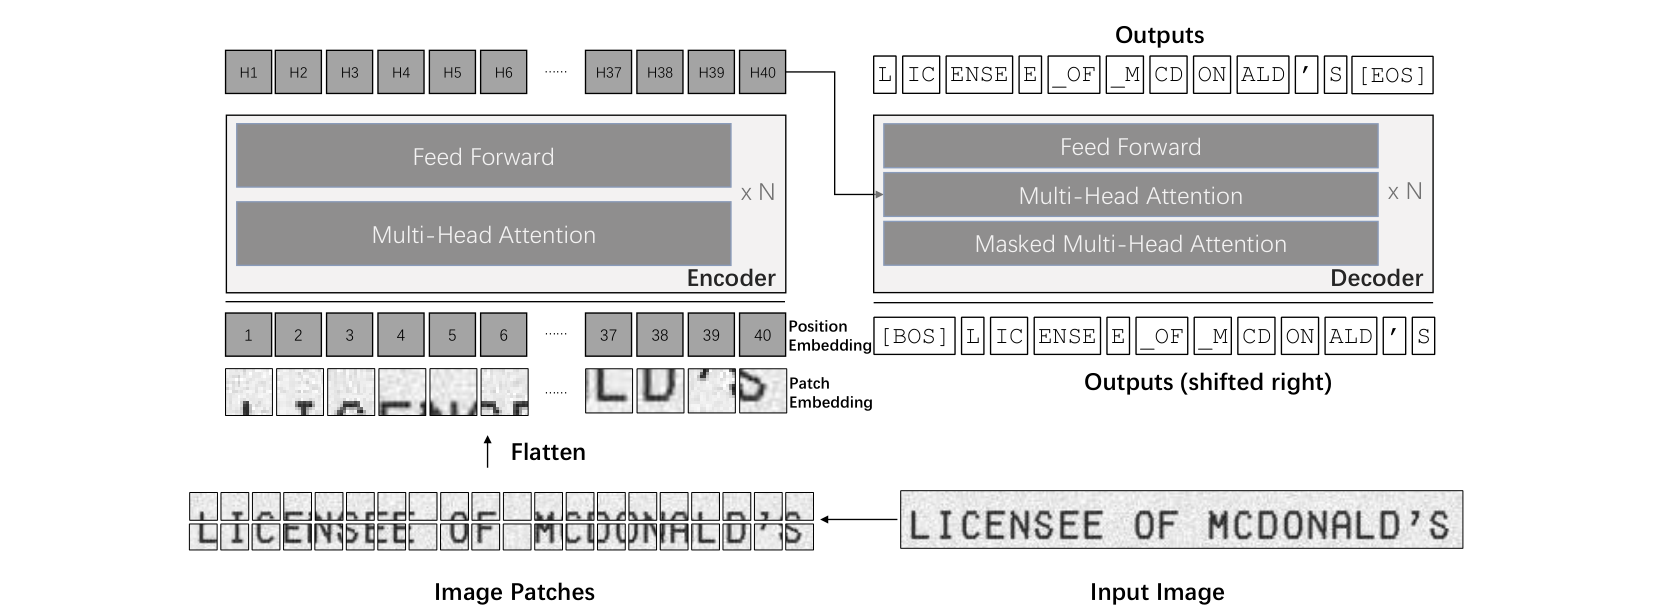
\includegraphics[width=\textwidth]{img/trocr_architecture_crop.png}
    \caption{Architecture hybride de TrOCR : l'image de la ligne (imprimée ou manuscrite) est découpée en patchs visuels traités par un encodeur Transformer, puis transcrite par un décodeur de texte. Extrait de \cite{li_trocr_2021}.}
    \label{fig:trocr_arch}
\end{figure}

Le principal avantage de ces approches hybrides est leur polyvalence. Un seul modèle traite l'ensemble des contenus de la page sans tri par un opérateur. En contrepartie, ces réseaux sont plus lourds car ils comptent plusieurs centaines de millions de paramètres \citep{li_trocr_2021}. Leur exécution nécessite donc une carte graphique (GPU) pour conserver une vitesse de lecture rapide.

Quelle que soit l'approche retenue (OCR, HTR ou hybride), envoyer une page entière au modèle de reconnaissance reste inefficace : la présence de tampons, de marges ou de cadres perturbe la lecture. Il est donc nécessaire de repérer d'abord les zones d'intérêt dans la page avant de lancer la transcription.




\subsection{La détection spatiale et l'analyse de mise en page par YOLO}

Envoyer directement la photo complète d'un document à un moteur de lecture pose un problème : la page contient des marges blanches, des tampons, des lignes de cadres et des annotations. Si le moteur essaie de tout lire sans tri, ce dernier perd du temps et produit du texte parasite. Il est donc important d'isoler d'abord les zones d'intérêt dans la page avant d'extraire le texte.

Le modèle YOLO (\textit{You Only Look Once}) \citep{redmon_yolo_2016, jiang_review_2022} a été conçu pour détecter des objets et des zones visuelles en un seul passage rapide sur l'image.

\begin{figure}[H]
    \centering
    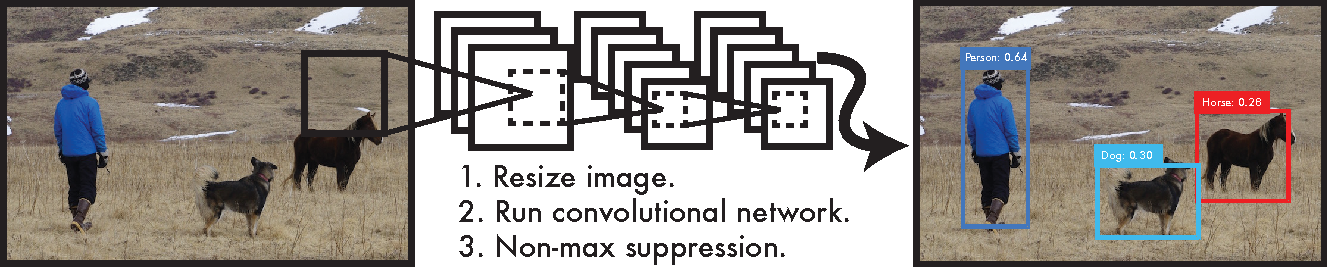
\includegraphics[width=0.8\textwidth]{img/yolo_system.pdf}
    \caption{Principe de détection de YOLO : traitement en un seul passage (\textit{Single-Shot}) sur une grille spatiale. Extrait de \cite{redmon_yolo_2016}.}
    \label{fig:yolo_architecture}
\end{figure}

La Figure~\ref{fig:yolo_architecture} illustre ce procédé. Dans un premier temps, l'image complète du document est redimensionnée pour être analysée d'un seul coup. Le réseau divise ensuite la page en une grille de cellules et calcule simultanément la position des boîtes englobantes et leur catégorie. Enfin, un filtre d'élimination des doublons (\textit{Non-Max Suppression}) ne conserve que le cadre le plus précis autour de chaque zone.

Pour garantir un bon cadrage cases et des tableaux, l'entraînement de YOLOv8 utilise la fonction de perte CIoU (\textit{Complete Intersection over Union}) \citep{zheng_ciou_2020} :

\begin{equation}
  \mathcal{L}_{CIoU} = 1 - IoU + \frac{\rho^2(\mathbf{b}, \mathbf{b}^{gt})}{c^2} + \alpha v
\end{equation}

Cette formule mesure la qualité du cadrage selon trois critères : le chevauchement ($IoU$) entre la boîte prédite et la vraie zone, l'écart de distance ($\rho^2 / c^2$) entre leurs centres respectifs, et la cohérence de la forme ($\alpha v$) pour préserver les proportions en hauteur et en largeur. Concrètement, l'entraînement cherche à réduire cette perte $\mathcal{L}_{CIoU}$ vers 0. Lorsque le chevauchement $IoU$ augmente, le terme $1 - IoU$ diminue. À l'inverse, si la distance $\rho$ entre les centres s'agrandit ou si les proportions se déforment (hausse de $v$), la perte augmente et pénalise le modèle, l'obligeant à recentrer le cadre et ajuster ses dimensions. Grâce à cette astuce, YOLOv8 ajuste le contour des zones, même lorsqu'il s'agit de lignes fines ou de petites cases.

Pour comprendre comment le réseau extrait ces caractéristiques visuelles étape par étape avant d'ajuster les cadrages, la Figure~\ref{fig:yolo_net} présente l’architecture du modèle.

\begin{figure}[H]
    \centering
    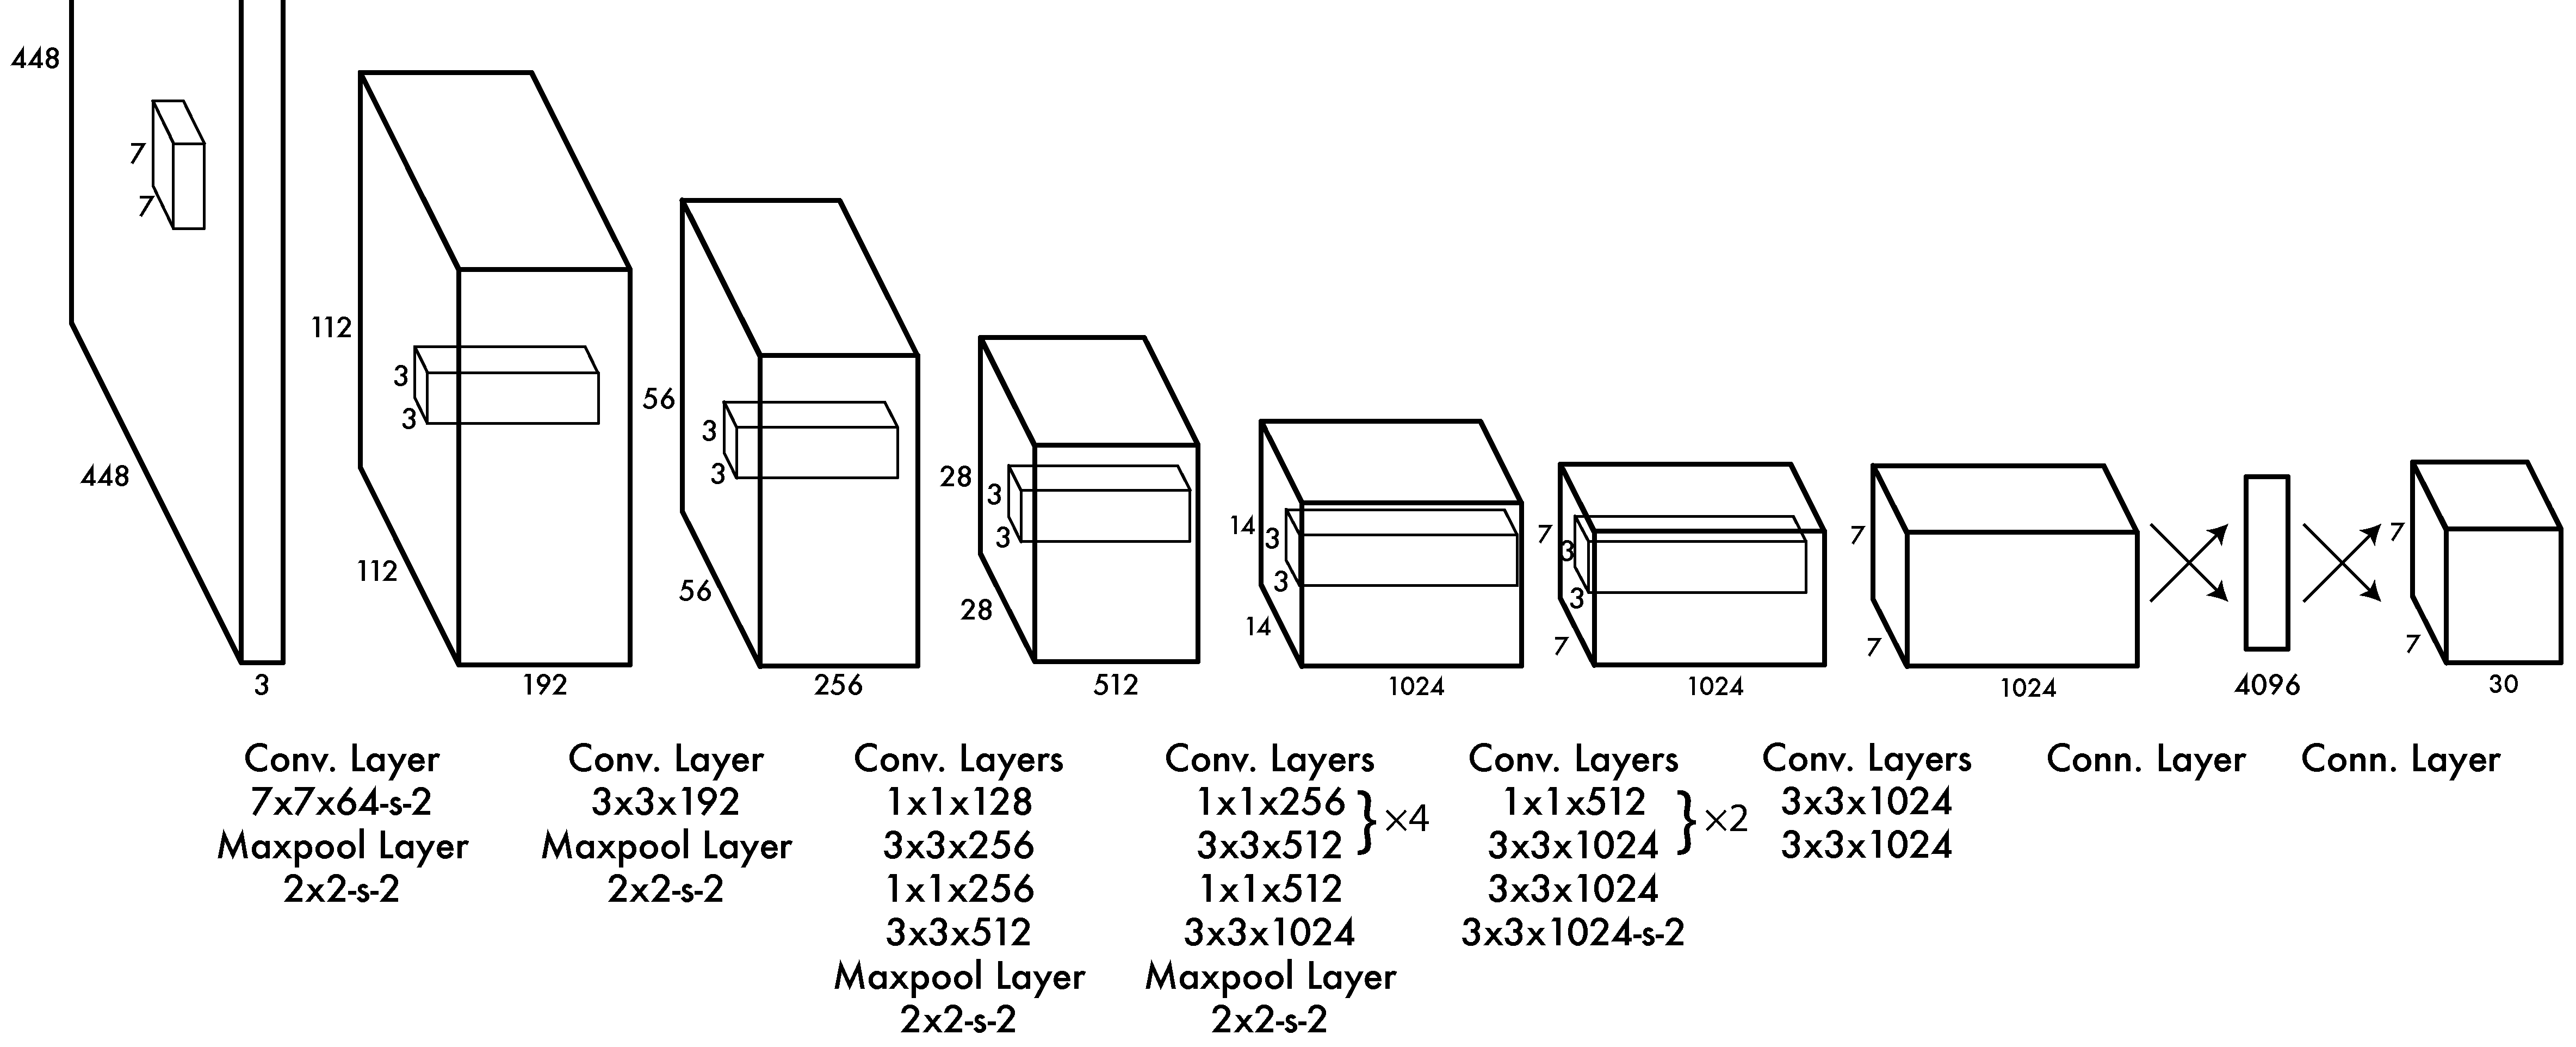
\includegraphics[width=\textwidth]{img/yolo_net.pdf}
    \caption{Architecture du réseau de convolution de YOLO. Extrait de \cite{redmon_yolo_2016}.}
    \label{fig:yolo_net}
\end{figure}

L'organisation du réseau de convolution responsable de la détection visuelle y est détaillée. L'image du document traverse d'abord une succession de couches de convolution qui repèrent les détails géométriques simples, pouvant être les lignes des tableaux, les angles ou encore les contours des cadres. Les couches suivantes combinent ces éléments pour reconnaître des blocs plus complexes, tels que des entêtes, des colonnes ou des cartouches. En parallèle, des opérations de sous-échantillonnage (\textit{max-pooling}) réduisent la taille spatiale pour préserver une vue globale sans alourdir les calculs. Enfin, les dernières couches du réseau convertissent ces caractéristiques visuelles en coordonnées spatiales(position, largeur et hauteur) et attribuent une catégorie à chaque zone identifiée.

Cette architecture permet à YOLO d'analyser rapidement la géométrie d'une page entière et d'isoler les zones d'intérêt.

Contrairement aux approches par modèles de détection classiques reposant sur des boîtes d'ancres pré-définies (*anchor-based*), la version v8 de YOLO utilise une architecture sans ancres (*anchor-free*). Ce choix simplifie l'apprentissage sur des documents administratifs aux formats non standard, car le réseau prédit directement les coordonnées du centre et les dimensions de chaque zone au lieu d'ajuster des cadres pré-formés. Sur des archives foncières où l'échelle des cartouches et l'emplacement des formulaires varient selon l'époque et l'imprimeur, cette flexibilité permet de détecter les zones utiles avec une meilleure précision qu'un simple découpage à coordonnées fixes.

Comme détaillé ultérieurement lors de l'explication de la chaîne de traitement (chapitre~\ref{sec:architecture}), cette étape de découpage spatial constitue le point d'entrée de toute l'analyse : elle préserve la mémoire de calcul en évitant de soumettre l'intégralité des images haute résolution aux modèles de lecture manuscrite.




Plutôt que de se reposer uniquement sur l'aspect visuel de la page comme YOLO, une autre approche consiste à utiliser des modèles multimodaux, capables de croiser le texte, la position des mots et l'image, comme par exemple LayoutLM \citep{xu_layoutlm_2020}.

\begin{figure}[H]
    \centering
    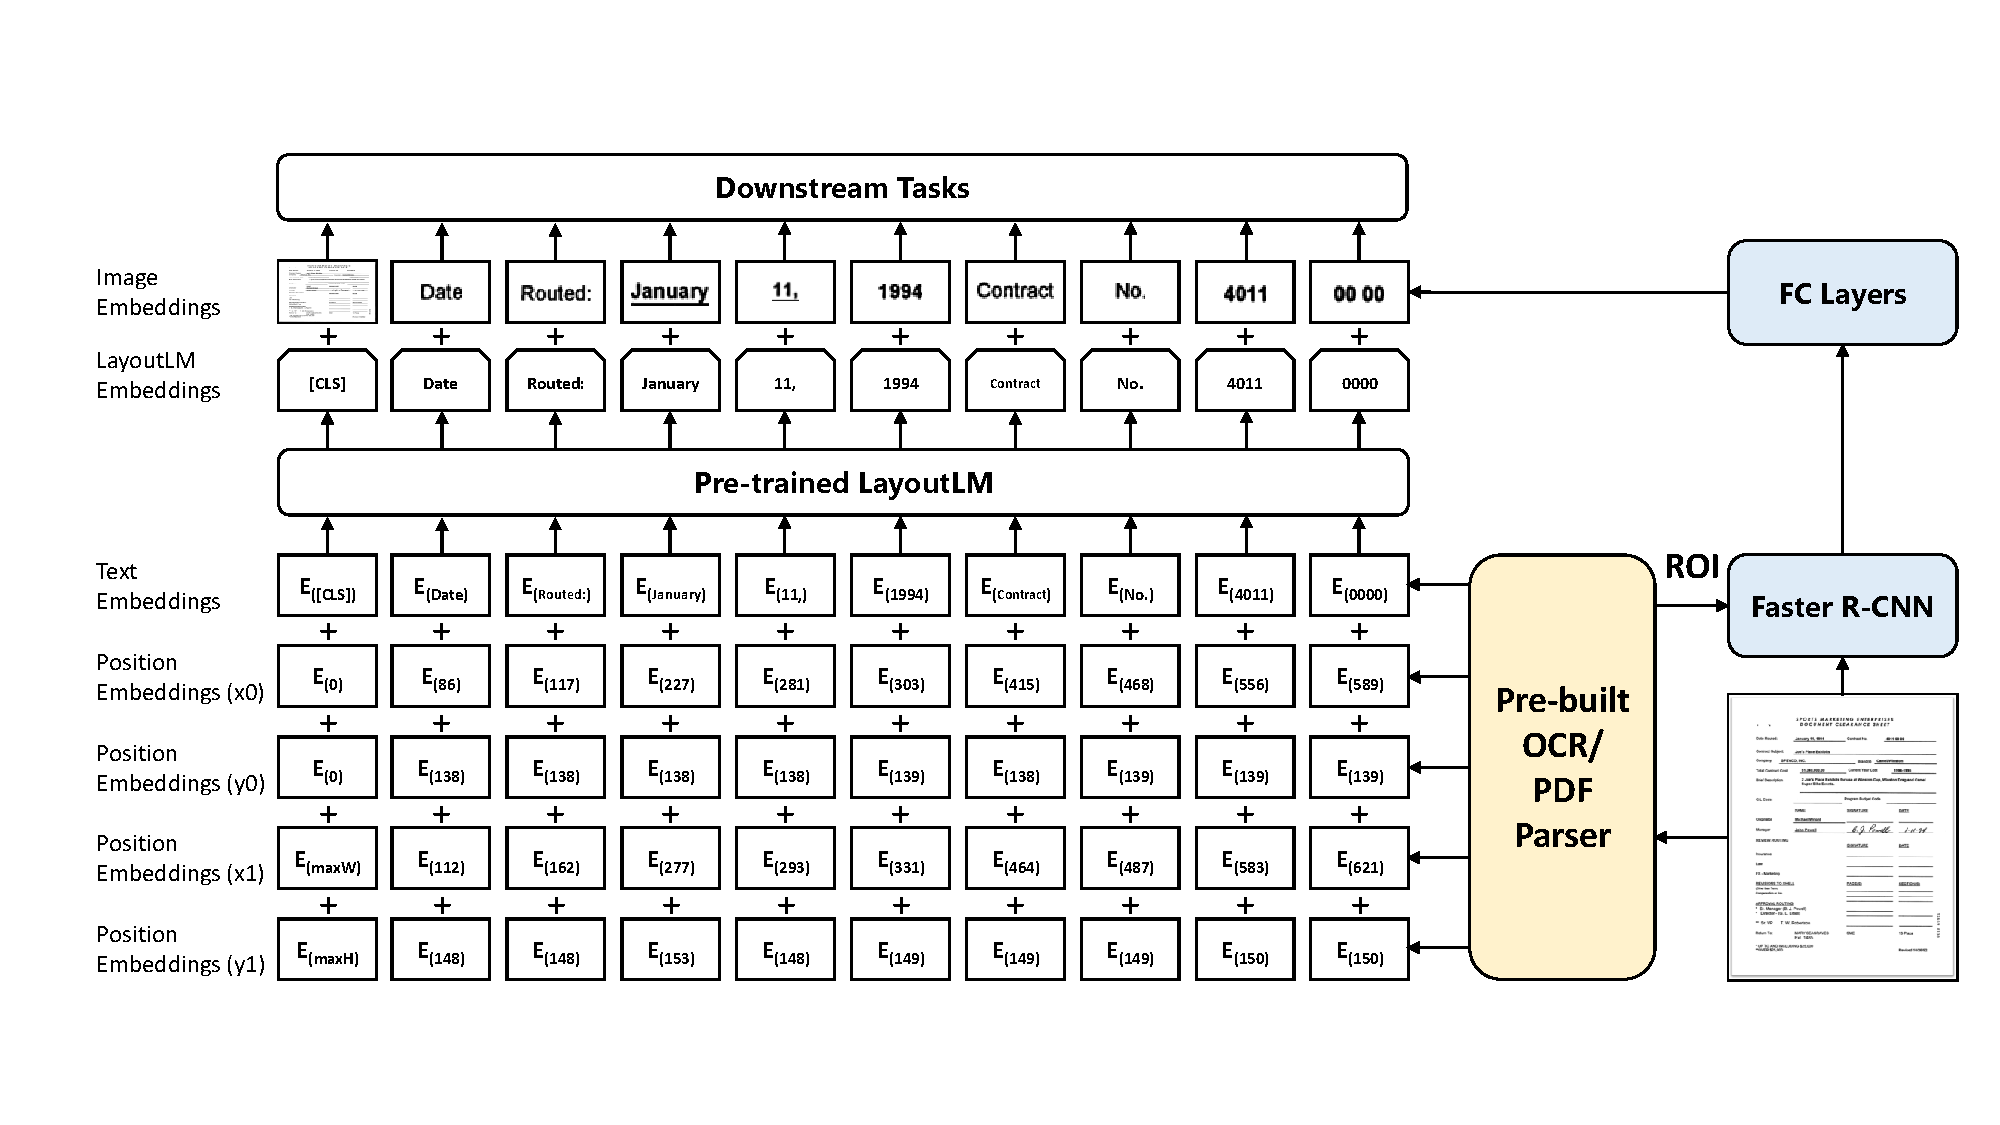
\includegraphics[width=\textwidth]{img/layoutlm_arch.pdf}
    \caption{Architecture de LayoutLM : combinaison du texte lu, de la position spatiale des mots sur la page et du signal visuel. Extrait de \cite{xu_layoutlm_2020}. Ce schéma est également disponible en grand format horizontal en \hyperref[ann:layoutlm]{Annexe B}.}
    \label{fig:layoutlm_architecture}
\end{figure}

Comme l'illustre le schéma de la Figure~\ref{fig:layoutlm_architecture}, ce modèle traite la page en faisant communiquer plusieurs canaux d'informations qui apparaissent à différents niveaux du diagramme.



En bas à droite du schéma, le document passe d'abord dans un moteur OCR préalable. Cet outil extrait les mots individuels (comme Date, January ou 1994) et calcule leurs coordonnées exactes sur la feuille, représentées par les quatre coins du cadre englobant $(x_0, y_0, x_1, y_1)$.

Au centre de l'architecture, chaque mot est transformé en un vecteur de texte (\textit{Text Embeddings}), auquel le modèle additionne directement quatre vecteurs de position (\textit{Position Embeddings}). Ces représentations spatiales indiquent où se situe le mot horizontalement et verticalement sur la page, ce qui permet au réseau Transformer (\textit{Pre-trained LayoutLM}) de comprendre la disposition en colonnes ou en tableaux.

En haut à droite du schéma, un réseau visuel (\textit{Faster R-CNN}) découpe l'image de chaque bloc pour extraire des caractéristiques visuelles (\textit{Image Embeddings}), comme la police d'écriture ou la présence de cadres. Ces informations visuelles sont ensuite ajoutées aux vecteurs de texte et de position pour produire la représentation finale du document.

Toutefois, cette architecture présente un point faible visible dès le début du schéma : la toute première brique repose entièrement sur le moteur OCR. Si cette lecture initiale échoue sur du texte manuscrit, des ratures ou une faible résolution, les mots transmis à la base de l'architecture sont erronés. Ces erreurs de texte se propagent ensuite dans tout le réseau Transformer et faussent la compréhension globale de la mise en page.

Pour mesurer l'impact de ces erreurs de texte sur les performances de LayoutLM, il est intéressant d'examiner la matrice de confusion mesurée par les auteurs du modèle (Figure~\ref{fig:layoutlm_confusion}).



\begin{figure}[H]
    \centering
    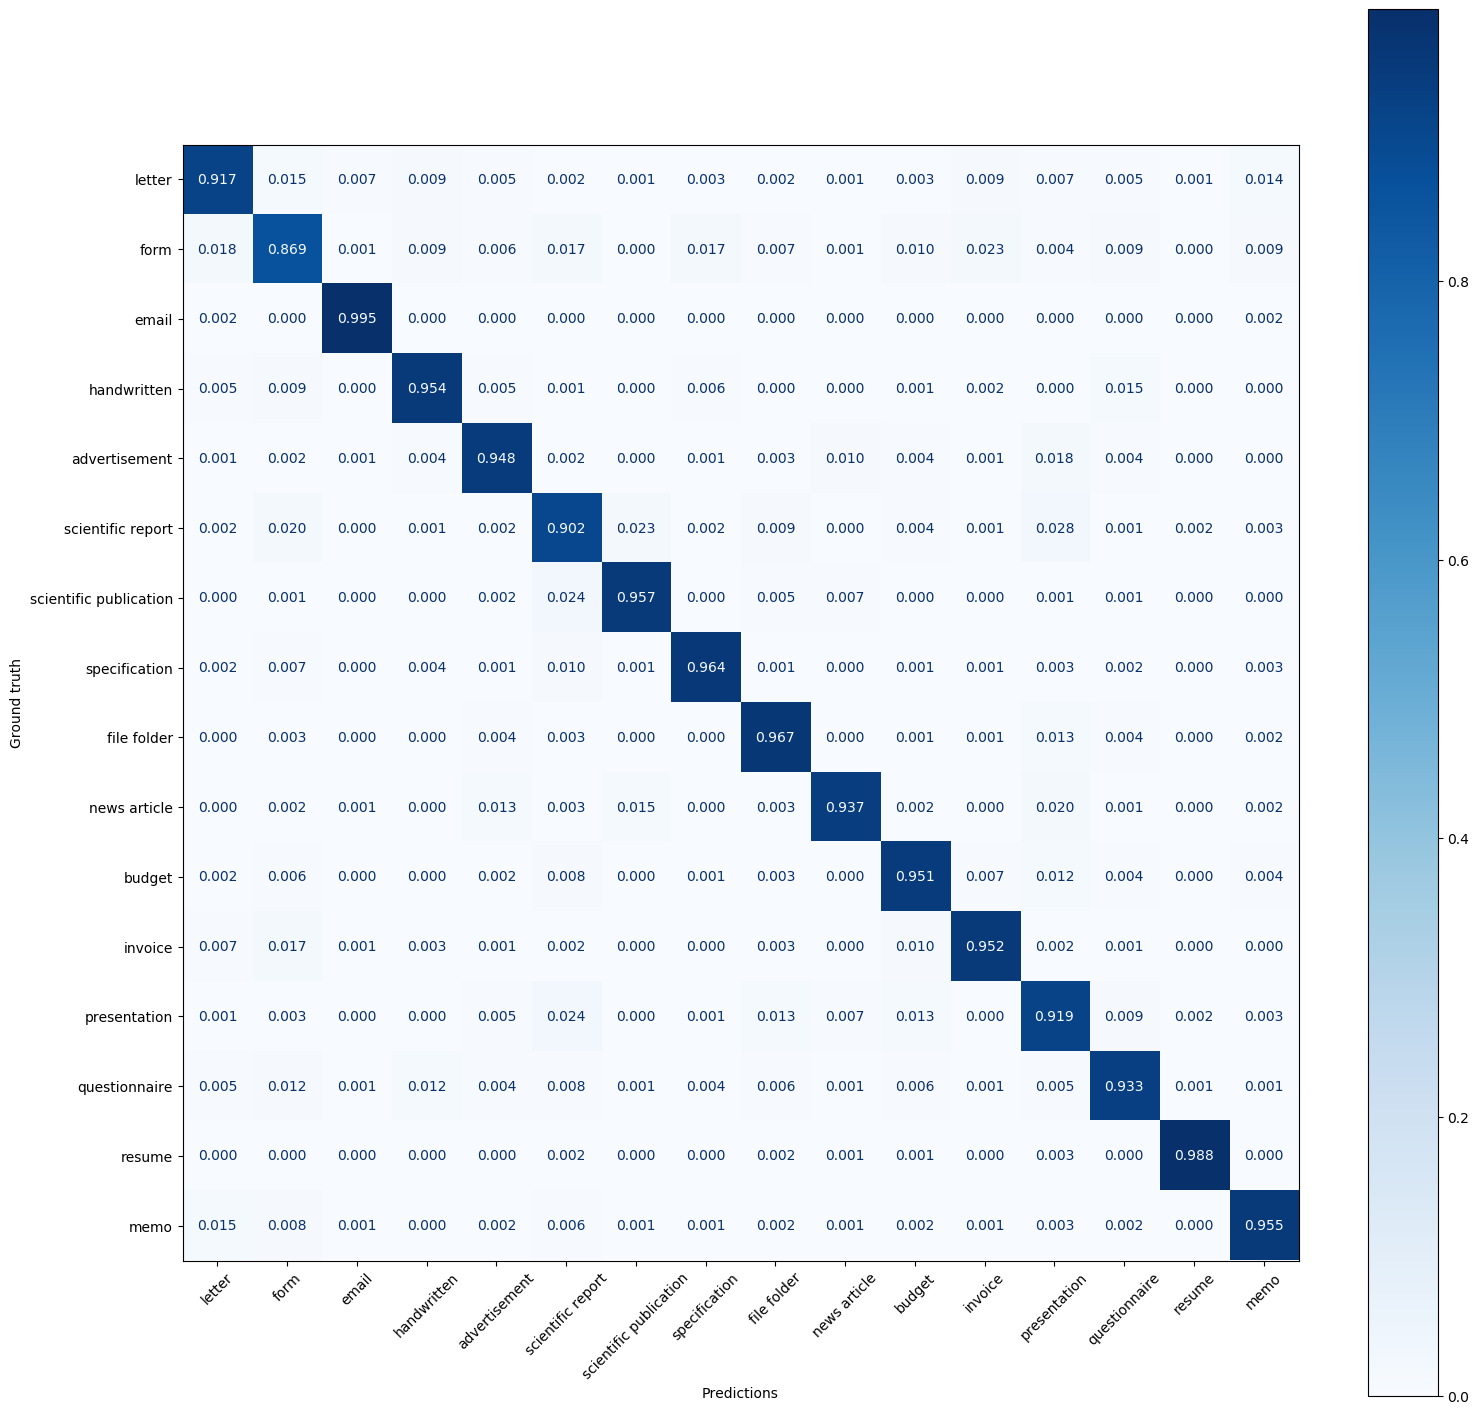
\includegraphics[width=0.65\textwidth]{img/layoutlm_confusion.png}
    \caption{Matrice de confusion de LayoutLM : la diagonale montre le taux de réussite pour chaque type de document, tandis que les cases hors diagonale révèlent les confusions causées par du texte mal reconnu. Extrait de \cite{xu_layoutlm_2020}. Cette matrice est également disponible en grand format horizontal en \hyperref[ann:layoutlm_confusion]{Annexe C}.}
    \label{fig:layoutlm_confusion}
\end{figure}


La Figure~\ref{fig:layoutlm_confusion} présente la matrice de confusion de LayoutLM. Ce tableau croisé permet d'analyser la précision du modèle en comparant la vraie catégorie de chaque document (affichée sur l'axe vertical) avec la catégorie prédite par le réseau (sur l'axe horizontal). Les cases situées sur la diagonale principale représentent les classements corrects, le bleu devenant plus foncé lorsque le score se rapproche de 1 (soit 100~\% de réussite).

L'observation de cette matrice met en évidence deux comportements très différents selon la nature des documents.

Dans les évolutions ultérieures comme LayoutLMv3, les auteurs ont simplifié cette architecture en supprimant la dépendance envers un moteur OCR externe pour l'étape d'analyse visuelle. LayoutLMv3 découpe directement la page scannée en petits patchs d'images (de taille 16 par 16 pixels) traités par un transformateur visuel (Vision Transformer), tout en alignant conjointement les jetons de texte et les positions spatiales. Cependant, cette avancée exige un volume d'entraînement considérable sur plusieurs millions de documents annotés. Pour des cabinets de géomètres disposant de fonds d'archives spécifiques et hétérogènes, le coût de réentraînement complet de telles architectures reste hors de portée par rapport à des approches plus modulaires.


D'une part, sur des documents imprimés comme les e-mails (99,5~\%), les CV (98,8~\%) ou les dossiers (96,7~\%), le modèle atteint d'excellents résultats. Dans ces cas, les mots reconnus par l'OCR (comme des entêtes d'e-mail ou des sections de CV) fournissent des repères fiables.

D'autre part, les performances diminuent sur des documents comme les formulaires (86,9~\%), les rapports scientifiques (90,2~\%) ou les courriers manuscrits (91,7~\%). Par exemple, la matrice indique que 2,3~\% des formulaires sont confondus avec des factures et 1,8~\% avec des courriers. Même si ces pourcentages d'erreur semblent faibles au premier abord, ils représentent rapidement une source d'erreur, ce qui peut nécessiter des corrections. 


Cette baisse de précision s'explique par la dépendance du modèle au texte. Lorsqu'un formulaire comporte des ajouts écris à la main, des cases cochées de manière irrégulière ou du texte dégradé, l'OCR préalable commet de nombreuses erreurs de lecture. En recevant ce texte bruité ou incomplet, le réseau de neurones de LayoutLM interprète mal la structure de la page et attribue le document à une mauvaise catégorie.

À l'inverse, un modèle de détection visuelle comme YOLO s'appuie uniquement sur la géométrie de la page (les lignes, les cadres et les colonnes) sans dépendre de la lecture du texte. Il n'est donc pas sensible à la présence d'écriture manuscrite ou de ratures pour repérer les blocs d'un document.








L'étape suivante consiste à passer du texte brut lu sur la page à une information structurée et exploitable.

\subsection{L'extraction d'entités et compréhension du texte}

Cette opération, appelée extraction d'entités nommées (NER pour \textit{Named Entity Recognition}), consiste à associer chaque mot ou groupe de mots à une catégorie précise.


Les outils de NER traditionnels (comme SpaCy ou CamemBERT) fonctionnent avec une liste fermée de catégories définies au moment de leur entraînement. Pour ajouter de nouvelles catégories spécifiques à un domaine, il faut annoter à la main des fichiers exemples puis réentraîner le modèle, ce qui demande du temps.

Pour contourner cette contrainte, le modèle GLiNER proposé par \citet{zaratiana_gliner_2024} introduit une approche capable de reconnaître de nouvelles catégories sur n'importe quel texte sans réentraînement préalable.

\begin{figure}[H]
    \centering
    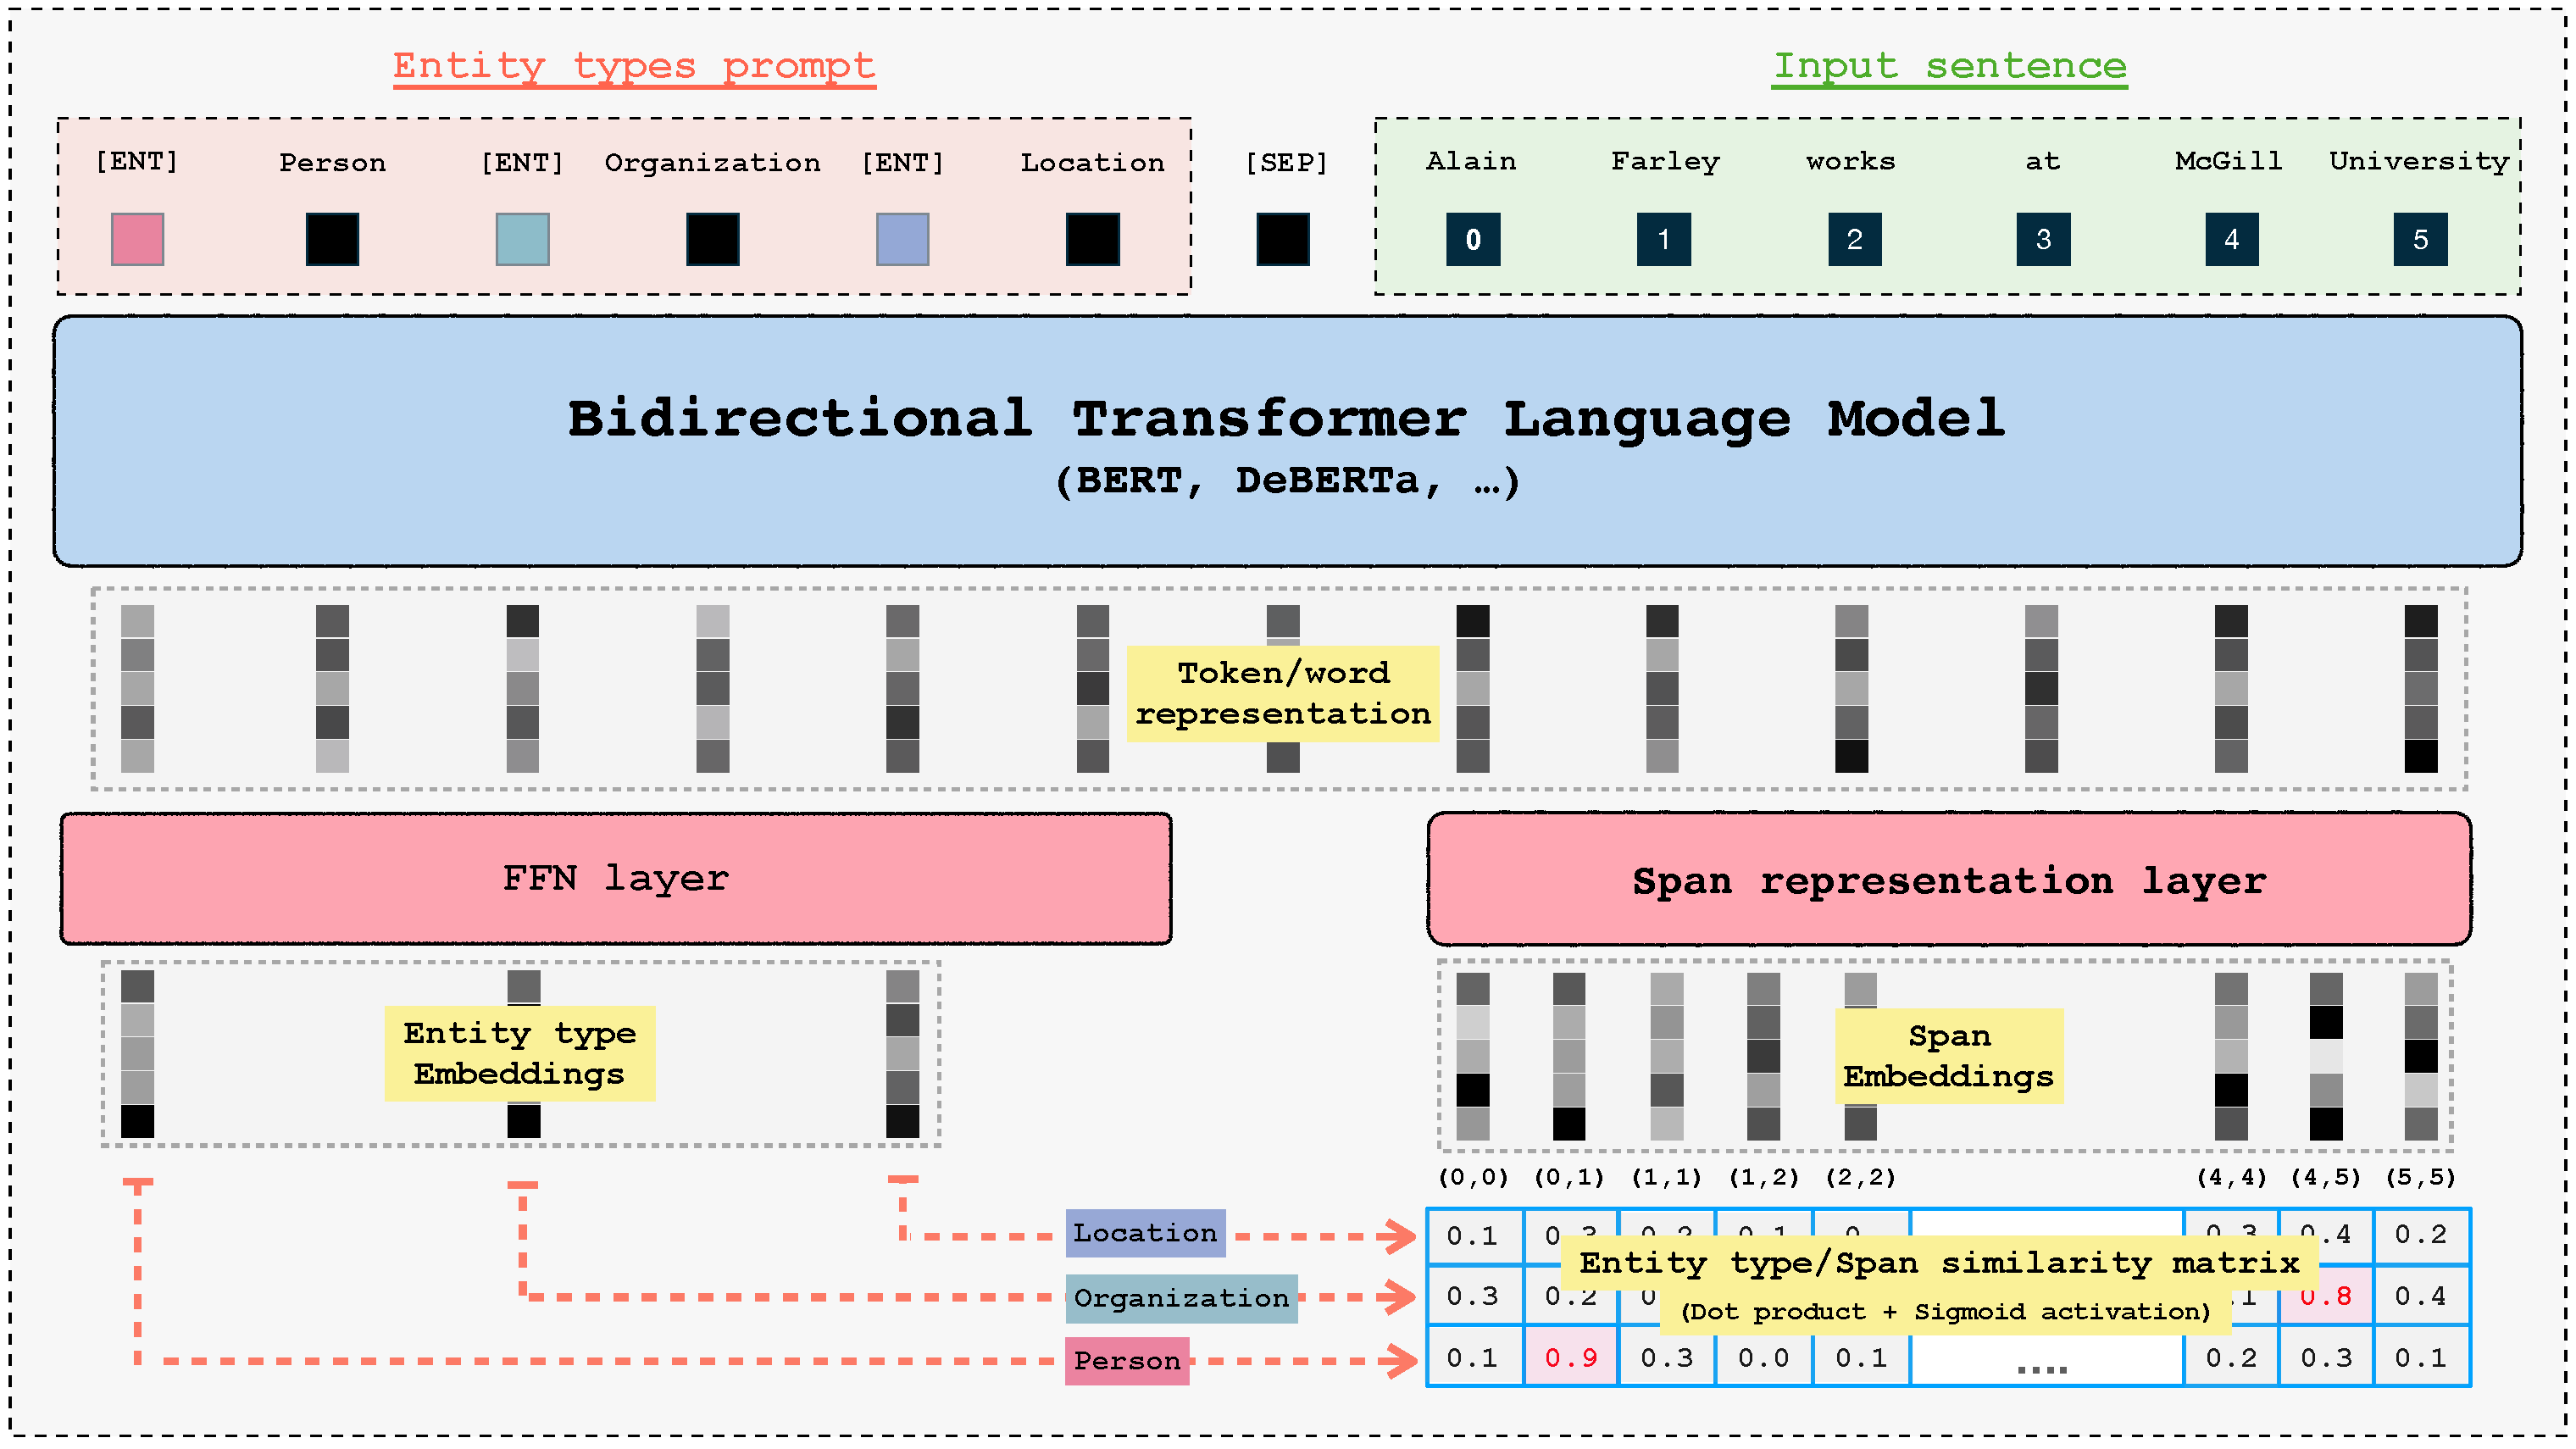
\includegraphics[width=0.9\textwidth]{img/gliner_gener.pdf}
    \caption{Architecture globale du modèle GLiNER : comparaison entre les morceaux de texte et les entités recherchées. Extrait de \cite{zaratiana_gliner_2024}. Ce schéma est également disponible en grand format horizontal en \hyperref[ann:gliner_architecture]{Annexe D}.}
    \label{fig:gliner_architecture}
\end{figure}

La Figure~\ref{fig:gliner_architecture} détaille l'organisation de ce réseau à travers plusieurs traitement.

En haut du schéma, le modèle reçoit deux entrées distinctes. À gauche, la consigne définit la liste des catégories recherchées (comme personne, organisation ou lieu), séparées par des balises. À droite, la phrase d'entrée contient le texte brut à analyser (par exemple \textit{Alain Farley works at McGill University}).

Au centre du schéma, l'ensemble traverse un modèle de langage bidirectionnel (comme DeBERTa). Ce réseau convertit simultanément la phrase et la liste des catégories en vecteurs numériques pour prendre en compte le contexte complet de chaque mot.

En bas du schéma, deux couches de projection calculent les caractéristiques finales. La branche de gauche produit la représentation numérique des catégories, tandis que la branche de droite regroupe les mots successifs en segments de texte, comme le nom complet \textit{Alain Farley}.

Enfin, le tableau bleu au bas de la figure présente la matrice de ressemblance. Le modèle calcule un produit scalaire entre chaque segment de texte et chaque catégorie recherchée. Dans l'exemple du schéma, le segment \textit{Alain Farley} s'associe à la catégorie des personnes avec un score élevé de 0,9, tandis que \textit{McGill University} correspond à la catégorie des organisations avec un score de 0,8.


Pour mettre en œuvre l'extraction d'entités avec GLiNER, deux facteurs doivent être pris en compte : la manière de formuler la consigne d'extraction et le choix du modèle de langage sous-jacent.

\begin{figure}[H]
    \centering
    \begin{minipage}{0.48\textwidth}
        \centering
        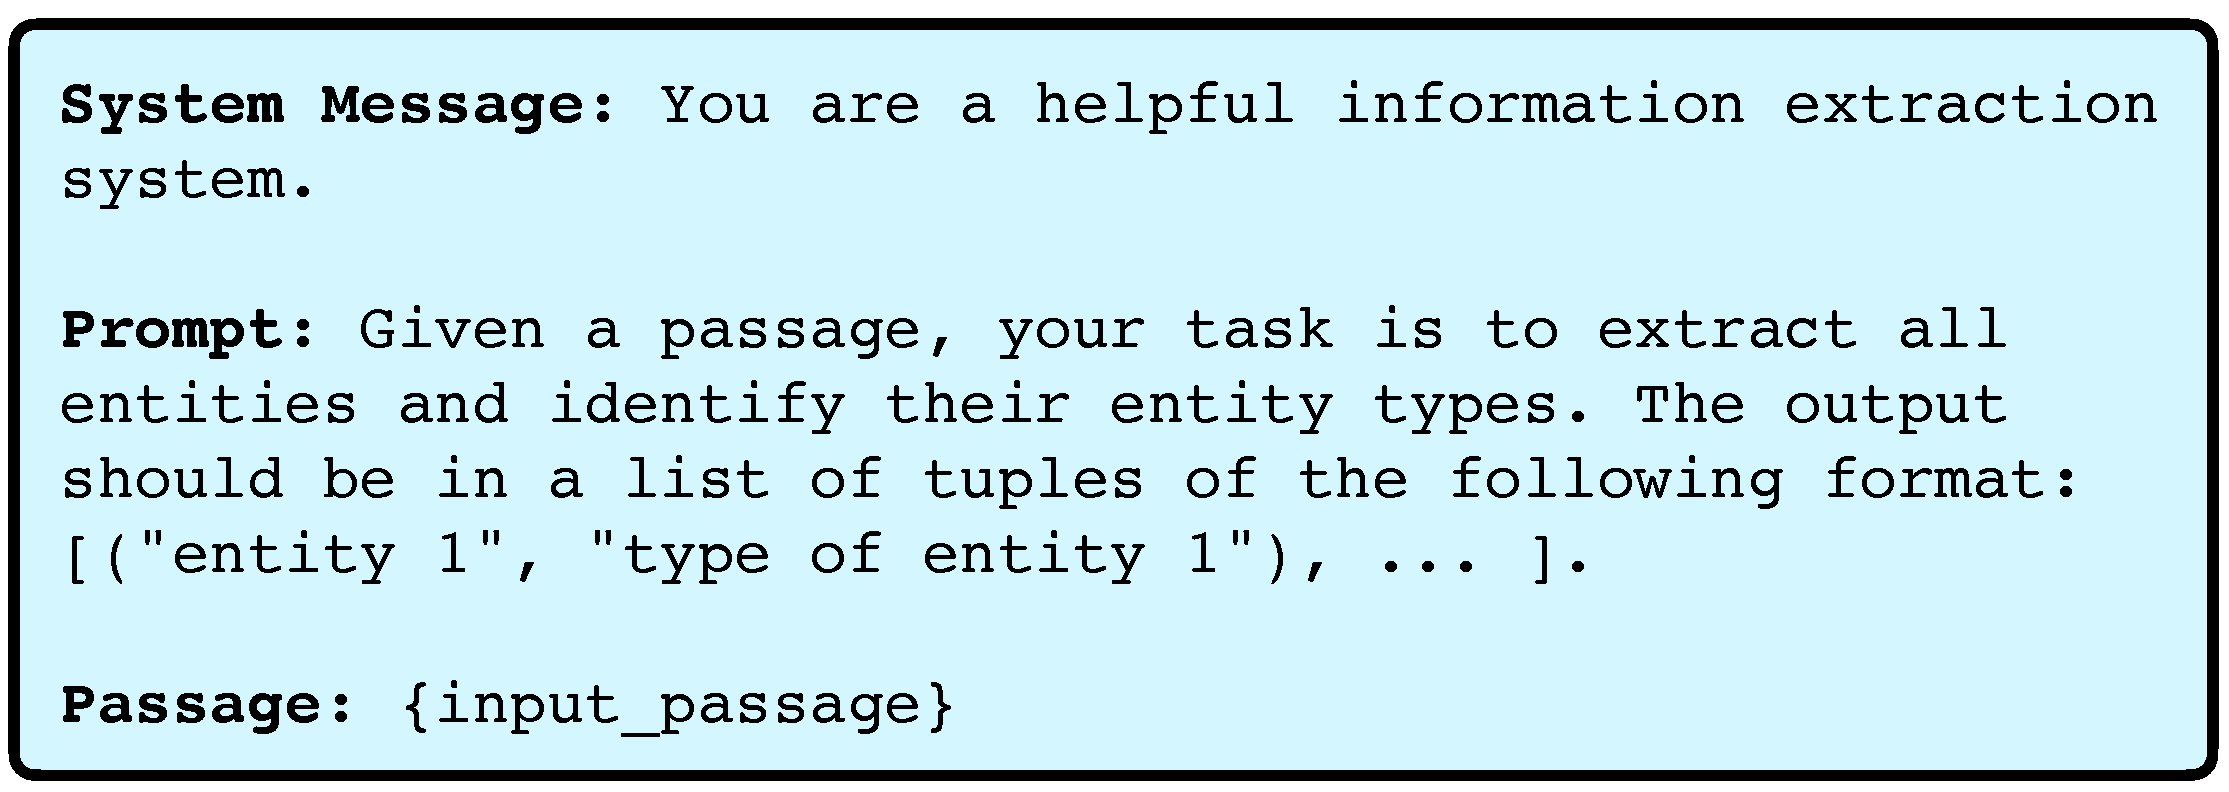
\includegraphics[width=\linewidth]{img/gliner_prompt.pdf}
        \caption{Format de la consigne transmise au modèle. Extrait de \cite{zaratiana_gliner_2024}.}
        \label{fig:gliner_prompt}
    \end{minipage}\hfill
    \begin{minipage}{0.48\textwidth}
        \centering
        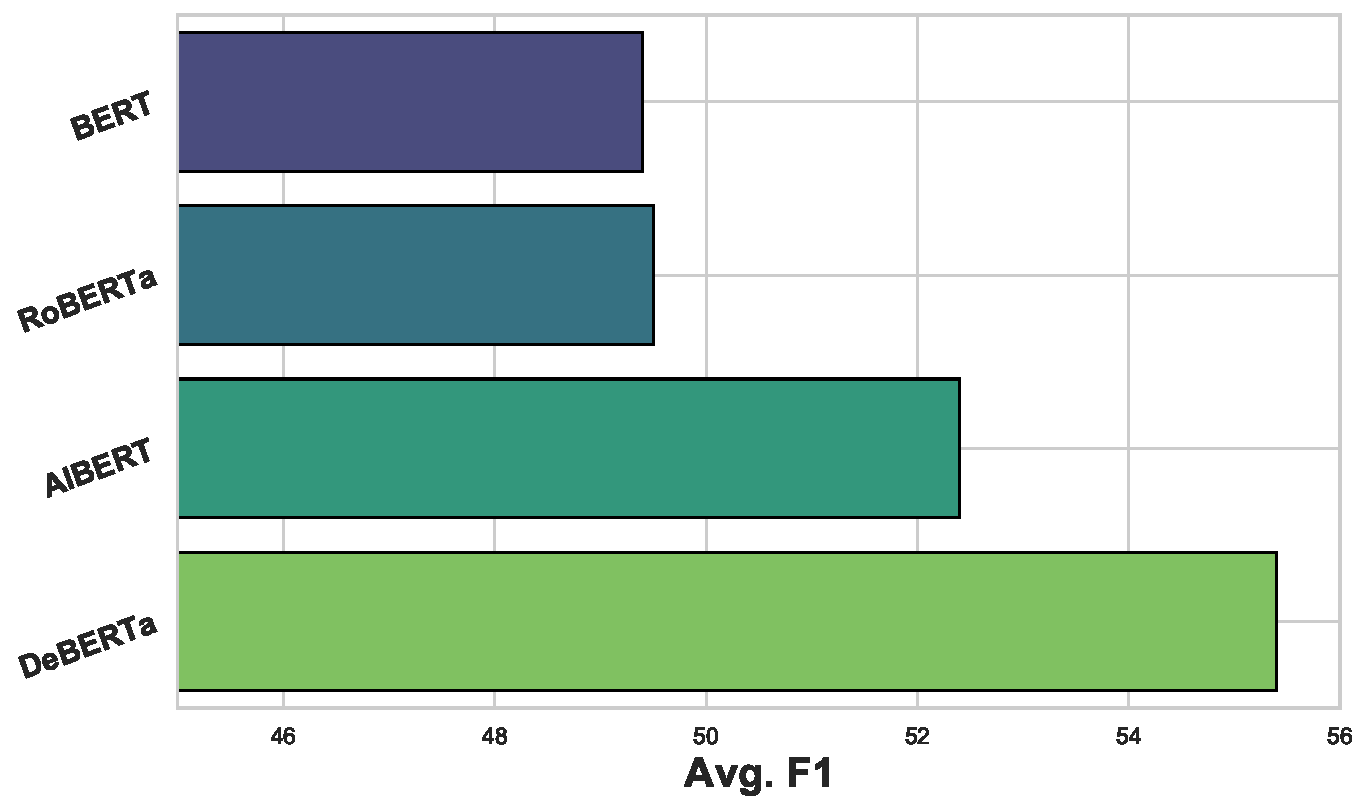
\includegraphics[width=\linewidth]{img/gliner_backbone.pdf}
        \caption{Comparaison des performances des modèles disponibles. Extrait de \cite{zaratiana_gliner_2024}.}
        \label{fig:gliner_backbone}
    \end{minipage}
\end{figure}

La Figure~\ref{fig:gliner_prompt} illustre la structure de la consigne transmise au modèle. Ce format permet de spécifier directement les noms des catégories recherchées sous forme de simples mots-clés, sans modifier le code du programme. Le schéma montre le rôle du message qui fixe la tâche globale, puis la liste des entités cibles. Le texte transcrit est inséré dans le champ d'entrée de la figure précédente pour être analysé.


La Figure~\ref{fig:gliner_backbone} provient des travaux de \citet{zaratiana_gliner_2024}. Les auteurs y évaluent l'impact du modèle de langage sous-jacent sur des jeux de données de référence en extraction d'entités sans réentraînement. La précision y est mesurée par le score F1, une métrique exprimée sur 100 qui combine à la fois la justesse des éléments extraits (la précision) et l'absence d'omissions. Ce graphique permet d'identifier l'architecture la plus efficace pour l'extraction d'informations. On observe que le réseau DeBERTa obtient le meilleur score F1 (55,5), surpassant des architectures comme AlBERT (52,4), RoBERTa (49,5) et BERT (49,4). 

Cependant, cette extraction repose sur la lisibilité du texte. En cas de document très abîmé ou d'écriture illisible, d'autres solutions doivent être envisagées.

\subsection{Les modèles Vision-Langage (VLM)} \label{sec:vlm_execution}


Lorsque certains documents sont très abîmés ou contiennent des mentions mal écrites, les moteurs de lecture par OCR et les modèles d'extraction par mots-clés peuvent atteindre leurs limites. Pour résoudre ces cas, une nouvelle classe d'outils issus de l'intelligence artificielle s'est développée : les modèles Vision-Langage (VLM pour \textit{Vision-Language Models}).

\begin{figure}[H]
    \centering
    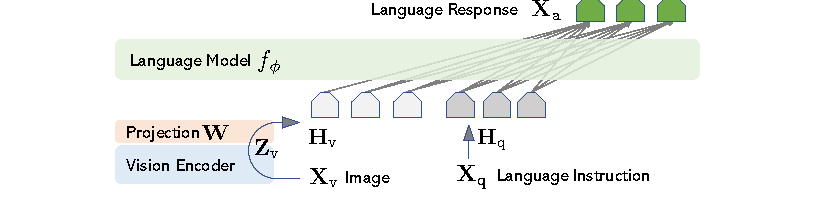
\includegraphics[width=0.85\textwidth]{img/llava_arch.pdf}
    \caption{Architecture interne du modèle Vision-Langage LLaVA. Extrait de \cite{liu_llava_2024}. Une version grand format est disponible en \hyperref[ann:llava_architecture]{Annexe E}.}
    \label{fig:vlm_architecture}
\end{figure}

La Figure~\ref{fig:vlm_architecture} présente l'architecture globale du modèle LLaVA issu des travaux de \citet{liu_llava_2024}. Le fonctionnement du réseau repose sur le couplage d'un encodeur visuel et d'un grand modèle de langage. En bas à gauche du schéma, la photo d'un extrait de document est transmise à l'encodeur visuel (Vision Encoder, fond bleu). Ce composant extrait les caractéristiques visuelles de l'image. Une couche de projection intermédiaire (Projection, fond orange) transforme ensuite ces données visuelles en une suite de représentations numériques compatibles avec le langage. En parallèle, à droite du schéma, la question posée (Language Instruction) est découpée en mots et transformée en texte. Les données visuelles et textuelles sont transmises simultanément au modèle de langage central (Language Model, fond vert), qui génère la réponse finale sous forme de texte.

Ces modèles existent sous deux formes d'exécution distinctes. D'une part, ceux accessibles en ligne (comme GPT-4 Vision ou Claude) proposent de bonnes capacités mais nécessitent le transfert des images vers des serveurs distants. D'autre part, des modèles ouverts et plus légers (comme LLaVA \citep{liu_llava_2024} ou Phi-3 Vision \citep{abdin_phi3_2024}) peuvent être exécutés directement en local sur la machine de l'utilisateur.

D'autres architectures VLM reconnues se distinguent par leur traitement des documents :
\begin{itemize}
  \item \textbf{Donut} \citep{kim_donut_2022} : modèle conçu spécifiquement pour la lecture de documents sans moteur OCR préalable. Ce dernier décode directement l'image pour produire une structure de texte (JSON). Il est plus rapide qu'un VLM classique, mais reste limité aux structures de formulaires connues.
  \item \textbf{Qwen-VL} \citep{bai_qwenvl_2023} : modèle  capable de traiter les images en résolution sans redimensionnement. Cela lui permet de lire de très petits caractères ou des textes denses sur de grands plans sans perte de définition.
  \item \textbf{Phi-3 Vision} \citep{abdin_phi3_2024} : modèle compact optimisé pour l'exécution locale sur un ordinateur standard en découpant les images HD en sous-blocs. Toutefois, comme son entraînement repose quasi exclusivement sur des jeux de données anglophones, ses performances chutent sur du texte en français, surtout pour un vocabulaire technique.
\end{itemize}

Bien que performants pour analyser des visuels de documents, les modèles Vision-Langage présentent deux contraintes. Le temps de calcul par image est plus long que celui d'un modèle d'extraction spécialisé comme YOLO ou GLiNER. De plus, sur des documents dégradés, ces modèles peuvent générer des réponses plausibles mais erronées, un phénomène appelé hallucination.

Dans ce projet, le choix s'est porté sur le modèle ouvert MiniCPM-V exécuté localement sous Ollama. Cette architecture combine un encodeur visuel SigLIP avec un modèle de langage compact. L'image de la zone d'intérêt est découpée en trames visuelles transformées en jetons textuels, permettant au réseau de répondre à des consignes ciblées en français. Pour réduire le temps de réponse et l'occupation mémoire, les poids du modèle ont été quantifiés en 4 bits, rendant l'inférence possible sur les processeurs graphiques standards du cabinet sans compromettre la compréhension des écritures manuscrites.



% A RELIRE
\subsection{La détection et l'extraction de tableaux dans les documents}
\label{subsec:table_detection}

Beaucoup de documents administratifs organisent leur contenu en colonnes et en lignes. Repérer la structure d'un tableau dans une image et en extraire le contenu est un problème distinct de la simple lecture de texte. Ce problème a été étudié depuis les travaux de \citet{duda_hough_1972} sur la détection de lignes géométriques.

Les premières approches reposent sur la transformée de Hough~\citep{duda_hough_1972}, qui repère les lignes horizontales et verticales dans l'image pour en déduire la grille du tableau. Cette technique fonctionne sur les tableaux imprimés dont les traits sont continus. En revanche, sur les documents anciens, les lignes de colonnes sont souvent discontinues ou absentes, remplacées par un simple alignement visuel des mots sans séparateur. \citet{canny_edge_1986} ont étendu cette approche par une détection préalable des contours, mais la limite sur les documents dégradés reste la même.

Des modèles entraînés à reconnaître la structure des tableaux ont ensuite été proposés. Le modèle \textit{Table Transformer} (TATR) de \citet{smock_table_2022} repose sur une architecture DETR (\textit{Detection Transformer}). Il analyse directement l'image et prédit la position de chaque ligne et colonne sous forme de boîtes englobantes, sans règles géométriques fixées à l'avance. Entraîné sur les jeux de données PubTables-1M et FinTabNet, il atteint un score F1 supérieur à 0,97 sur des tableaux imprimés normalisés. \citet{chi_complicated_2019} s'intéressent aux tableaux avec des cellules fusionnées et montrent que les architectures par décodage de graphe surpassent les approches par détection d'objets sur ces configurations.

\begin{figure}[H]
    \centering
    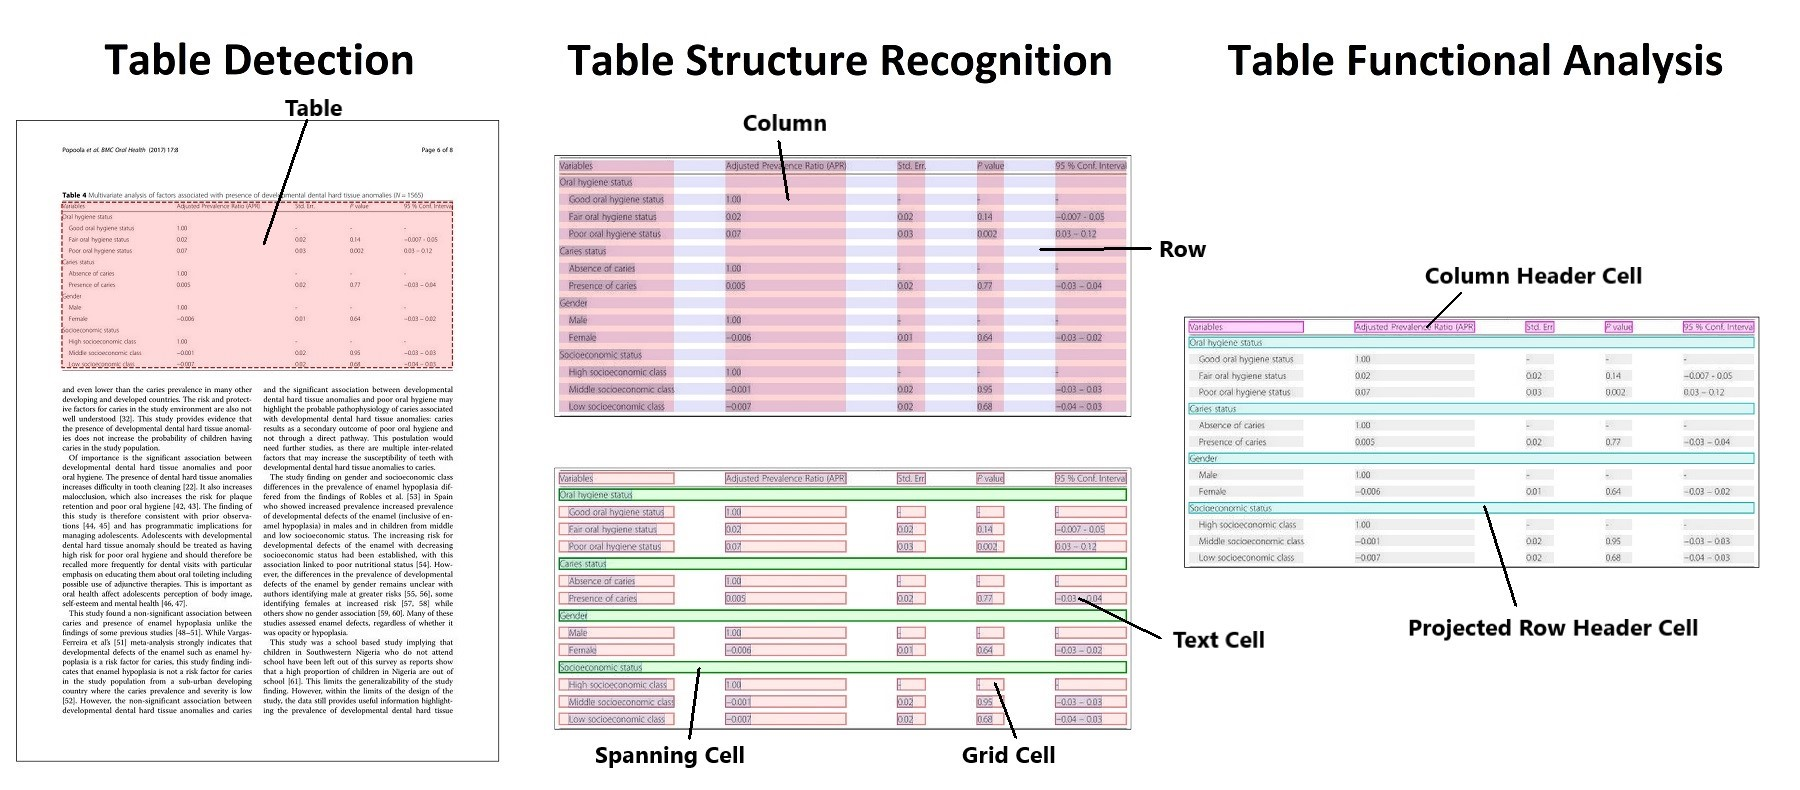
\includegraphics[width=\textwidth]{img/table_transformer_overview.png}
    \caption{Les trois tâches du Table Transformer de \citet{smock_table_2022} : détection de la table dans la page (gauche), reconnaissance de sa structure en lignes et colonnes (centre), et analyse fonctionnelle des types de cellules (droite). Source : \citet{microsoft_tatr_github}. Une version grand format est disponible en \hyperref[ann:table_transformer]{Annexe F}.}
    \label{fig:table_detection_overview}
\end{figure}

Sur des documents anciens numérisés à basse résolution, ces modèles se heurtent aux mêmes problèmes que les méthodes classiques. Les cellules ne sont parfois séparées que par un espace, et les plis du papier peuvent être lus à tort comme des séparateurs. \citet{zhong_image-based_2019} montrent que la position spatiale des blocs de texte, combinée à une analyse des proximités horizontales et verticales, est une alternative robuste quand les séparateurs visuels sont absents.

Dans les registres d'archives historiques où la séparation des colonnes repose sur un alignement visuel, l'analyse de la densité horizontale des projections de texte permet de détecter les espacements (zones blanches verticales). L'algorithme calcule l'histogramme des projections verticales des boîtes de texte sur la largeur de la page et identifie les creux de densité correspondant aux séparations naturelles entre les colonnes de données.

Pour compenser les décalages de ligne sur les registres, les coordonnées verticales des centroïdes des blocs de texte sont regroupées par un algorithme de clustering unidimensionnel (DBSCAN). Ce regroupement permet de rattacher chaque mot à sa ligne d'origine même si le rédacteur a écrit de manière oblique ou non rectiligne.

Cette analyse de la mise en page des tableaux est importante pour exploiter les répertoires d'anciens géomètres, comme présenté au chapitre~\ref{sec:architecture}. Elle permet l'alignement des données avant d'alimenter les modules suivants du projet.


Dans ce projet, les documents traités se répartissent en deux cas. Les formulaires DMPC imprimés ont des cases délimitées par des traits continus : la détection par boîtes englobantes via YOLOv8 suffit (chapitre~\ref{sec:architecture}). Les registres manuscrits, eux, organisent les données en colonnes sans trait visible. Dans ce second cas, ni la transformée de Hough ni le Table Transformer ne s'appliquent directement. La solution retenue combine la détection des blocs de texte par EasyOCR et leur regroupement par proximité verticale, comme détaillé pour la numérisation des registres au chapitre~\ref{sec:fiabilisation}.


\subsection{Métriques d'évaluation de la reconnaissance de texte}
\label{subsec:metrics_ocr}

Pour comparer les performances des modèles d'OCR, de HTR et d'extraction d'entités, la littérature scientifique s'appuie sur plusieurs métriques standardisées.

Le taux d'erreur sur les caractères (\textit{Character Error Rate} ou CER) mesure la proportion de caractères mal transcrits par rapport à la vérité terrain. Il repose sur la distance de Levenshtein au niveau des caractères :

\begin{equation}
  \text{CER} = \frac{S + D + I}{N}
\end{equation}

où $S$ est le nombre de substitutions, $D$ le nombre de suppressions, $I$ le nombre d'insertions et $N$ le nombre total de caractères dans le texte de référence. Un CER de 0\,\% indique une transcription parfaite, tandis qu'un CER inférieur à 5\,\% est considéré comme bon pour du texte manuscrit.

Le taux d'erreur sur les mots (\textit{Word Error Rate} ou WER) s'appuie sur le même principe, mais calculé au niveau des mots complets :

\begin{equation}
  \text{WER} = \frac{S_w + D_w + I_w}{N_w}
\end{equation}

où $S_w$, $D_w$ et $I_w$ représentent respectivement les substitutions, suppressions et insertions de mots entiers, et $N_w$ le nombre total de mots. Le WER est plus sévère que le CER, car une seule lettre de différence rend le mot entier faux.
% >>>>>>>>>>>>>>>>>>>

\textbf{Précision, Rappel et Score F1.} Pour l'extraction d'entités (comme la détection des noms de communes ou des numéros de parcelles par GLiNER), les métriques habituelles sont la précision ($P$), le rappel ($R$) et le score F1 ($F_1$) :

\begin{equation}
  P = \frac{TP}{TP + FP}, \quad R = \frac{TP}{TP + FN}, \quad F_1 = 2 \times \frac{P \times R}{P + R}
\end{equation}

où $TP$ désigne les vrais positifs (entités correctement extraites), $FP$ les faux positifs (entités attribuées à tort) et $FN$ les faux négatifs (entités manquées). Le score F1 combine précision et rappel en une valeur unique comprise entre 0 et 1 (ou 0\,\% et 100\,\%).
% >>>>>>>>>>>>>>>>>>>


\subsection{Synthèse des approches de l'état de l'art}




Chaque technologie étudiée dans ce chapitre répond à une tâche précise de l'analyse de document, qu'il s'agisse d'isoler des zones, de lire du texte ou d'en comprendre le sens. Le Tableau~\ref{tab:comparaison_modeles} regroupe ces différentes méthodes afin de comparer leur fonctionnement, leurs avantages et leurs limites, avec pour objectif de selectionner le plus propice au cas d'étude.

\begin{table}[H]
  \centering
  \small
  \renewcommand{\arraystretch}{1.35}
  \resizebox{\textwidth}{!}{%
  \begin{tabular}{@{} l p{3.4cm} c p{4.2cm} p{4.2cm} @{}}
    \toprule
    \textbf{Modèle} & \textbf{Méthode utilisée} & \textbf{Ressources} & \textbf{Points forts} & \textbf{Limites principales} \\
    \midrule
    Tesseract v5 & Analyse par caractères & CPU & Rapide et économe en mémoire. & Précision très faible sur le manuscrit. \\
    
    PyLaia / TrOCR & Réseau convolutif et Transformer & ~4 Go GPU & Forte précision sur le manuscrit. & Nécessite d'isoler les lignes au préalable. \\
    
    YOLOv8 & Détection d'objets spatiale & < 2 Go GPU & Détection visuelle très rapide et robuste. & Isole les zones sans lire le texte. \\
    
    LayoutLMv3 & Modèle multimodal vision-texte & ~8 Go GPU & Analyse conjointe de la forme et des mots. & Sensible aux erreurs de lecture initiale. \\
    
    GLiNER & Comparaison de représentations & ~2 Go GPU & Identification d'entités sans réentraînement. & Dépend de la propreté du texte transmis. \\
    
    Donut & Décodage visuel direct  & ~4 Go GPU & Extraction  sans OCR externe. & Limité aux types de fichiers connus. \\
    
    Qwen-VL & VLM à résolution dynamique & ~8 Go GPU & Lecture précise des détails et petits textes. & Temps de calcul élevé sur grand format. \\
    
    LLaVA / Ollama & Modèle Vision-Langage local & > 8 Go GPU & Raisonnement visuel direct en local. & Calcul lent et risque d'hallucination. \\
    \bottomrule
  \end{tabular}%
  }
  \caption{Synthèse comparative des technologies d'analyse de documents.}
  \label{tab:comparaison_modeles}
\end{table}

Pour comparer ces outils, il faut prendre en compte la machine de test. L'ensemble des essais s'appuie sur une configuration standard équipée d'un processeur Intel Core i7, de 32 Go de RAM et d'une carte graphique NVIDIA de 8 Go (VRAM), ce matériel constitue le cas d'étude, la puissance variant que très légèrement entres les postes du cabinet. 

Cette configuration matérielle influence directement le choix des modèles du Tableau~\ref{tab:comparaison_modeles}. Les outils légers comme YOLOv8 et GLiNER occupent moins de 2 Go de mémoire graphique et répondent presque instantanément. PyLaia utilise environ 4 Go pour lire une ligne en moins d'une seconde. À l'inverse, les modèles plus lourds comme LayoutLMv3 et LLaVA demandent beaucoup plus de ressources. Avec Ollama, LLaVA prend environ 4,8 secondes par extrait. De plus, son risque principal reste l'hallucination : sur un texte très abîmé, le modèle a parfois tendance à inventer une réponse crédible au lieu de signaler qu'il n'arrive pas à lire.

Pour compléter ces observations, la Figure~\ref{fig:benchmark_comparatif} compare la précision de chaque méthode (en bleu) et son temps de traitement moyen par zone (en orange). Ces valeurs sont issues des tests présentés dans les articles scientifiques sur des formulaires administratifs, des registres manuscrits et des documents de référence.

\begin{figure}[H]
    \centering
    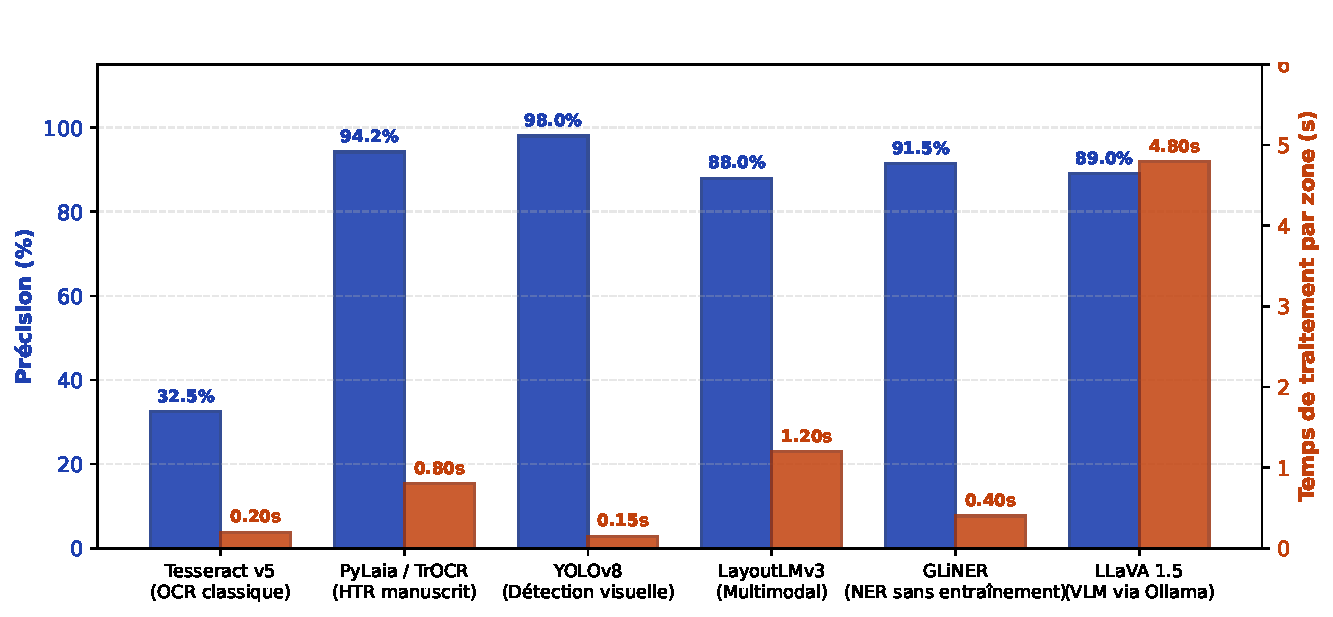
\includegraphics[width=0.92\textwidth]{img/benchmark_comparatif_modeles.pdf}
    \caption{Graphique comparatif de la précision et du temps de traitement moyen par zone selon les architectures étudiées (\cite{smith_tesseract_2007}, \cite{li_trocr_2021}, \cite{jiang_review_2022}, \cite{bajrami_comprehensive_2023}, \cite{zaratiana_gliner_2024}, \cite{liu_llava_2024}).}
    \label{fig:benchmark_comparatif}
\end{figure}

YOLOv8 se montre très rapide (0,15 seconde par zone) et efficace pour repérer les emplacements (98,0\%). Il permet d'isoler rapidement les tampons, les signatures ou les tableaux sans lire le texte. À l'opposé, un modèle comme LLaVA demande environ 4,80 secondes par zone en local. Comme expliqué dans la Section~\ref{sec:vlm_execution}, l'utilisation de services en ligne pose la question de la confidentialité des données d'archives. Même si LLaVA obtient 89,0\% de réussite grâce au raisonnement visuel direct, ce temps de calcul élevé constitue sa limite principale sur des volumes importants de documents.

L'analyse des articles de la littérature confirme ces résultats. Les moteurs de lecture classiques comme Tesseract \citep{smith_tesseract_2007} fonctionnent bien sur des imprimés propres, mais leur taux d'erreur dépasse 30\% dès que le texte est manuscrit. À l'inverse, les modèles de reconnaissance manuscrite (HTR) comme TrOCR \citep{li_trocr_2021} et PyLaia \citep{tarride_improving_2024} lisent très bien l'écriture manuelle (moins de 6\% d'erreur, d'après la synthèse de \citet{alkendi_advancements_2024}), mais ils exigent que le texte leur soit transmis ligne par ligne.

Pour découper ces lignes sans problématiques de mise en page, la détection avec YOLOv8 \citep{redmon_yolo_2016, jiang_review_2022} permet d'isoler proprement chaque zone de texte avant la lecture.


Du côté de la compréhension du texte, les modèles comme LayoutLM \citep{xu_layoutlm_2020} essaient d'analyser à la fois la forme et les mots. Cependant, les travaux comparatifs de \citet{bajrami_comprehensive_2023} montrent que LayoutLM reste très sensible aux fautes de lecture de l'OCR : dès que le texte extrait contient des erreurs, la compréhension globale baisse nettement (autour de 88,0\% au mieux). C'est ce qui a poussé les chercheurs à développer des modules de correction comme LayoutLM-Critic \citep{xu_layoutlm-critic_2022}.

De leur côté, des outils comme GLiNER permettent d'extraire des entités (communes, dates, parcelles) sans réentraînement, avec un score F1 de 91,5\%, à condition que le texte fourni soit propre.

Cette analyse montre qu'aucune technologie existante ne peut traiter seule l'ensemble des archives du projet. L'OCR classique échoue sur l'écriture manuscrite, les modèles HTR exigent un découpage préalable des lignes, LayoutLM reste bloqué par les erreurs de lecture, et les VLM demandent trop de temps de calcul. C'est pourquoi il convient d'associer plusieurs de ces approches au sein du projet, en utilisant chaque outil uniquement là où il est le plus efficace (chapitre~\ref{sec:architecture}).


\subsection{Choix des méthodes retenues}

Afin de répondre aux contraintes du projet et de trouver une solution pour minimiser les limites de chaque modèle, une méthode combinant quatre outils a été retenue :

\begin{itemize}
  \item Ultralytics YOLOv8 pour la segmentation spatiale : ce modèle découpe visuellement les zones d'intérêt sur les formulaires imprimés sans dépendre du texte.
  \item EasyOCR et PyLaia pour l'extraction textuelle : EasyOCR lit les parties imprimées tandis que PyLaia traite l'écriture manuscrite des registres.
  \item GLiNER pour le repérage des entités : il identifie les champs clés (commune, date, section, parcelles) dans le texte extrait sans réentraînement préalable.
  \item Ollama avec MiniCPM-V en secours local : ce modèle VLM s'exécute uniquement sur les zones incertaines pour lever les ambiguïtés de lecture.
\end{itemize}

Cette architecture hybride garantit le respect du secret professionnel en fonctionnant intégralement en local (chapitre~\ref{sec:analyse_metier}). Elle prépare les données pour la phase de fiabilisation et de validation par l'opérateur (chapitre~\ref{sec:fiabilisation}), avant l'exportation vers le portail Géofoncier (chapitre~\ref{sec:integration}).


Pour le repérage des zones, le modèle YOLOv8 a été choisi. Son rôle est d'isoler les cases des communes, les dates, les tableaux de parcelles ainsi que les tampons permettant d'identifier le géomètre-expert ayant réalisé la mission. Ce choix s'explique par sa rapidité (0,15 seconde par zone), sa faible consommation de mémoire graphique (moins de 2 Go) et son insensibilité au texte. Il permet de découper proprement les images sans dépendre d'un gabarit fixe, et de préparer ainsi les extraits d'images nécessaires au fonctionnement du modèle PyLaia.


Pour la transcription du texte manuscrit, le modèle HTR PyLaia a été sélectionné. Alors que l'OCR classique comme Tesseract échoue sur l'écriture manuelle, PyLaia lit les registres manuscrits avec précision dès que les lignes lui sont transmises sous forme de découpes isolées par YOLO.

Pour l'extraction des données clés (noms de communes, dates, numéros de parcelles), l'outil GLiNER a été retenu. Contrairement aux modèles comme LayoutLM qui deviennent inefficaces lorsque le texte contient des fautes, GLiNER identifie les entités sans entraînement spécifique et réduit le risque de faux positif, comme présenté dans ce chapitre.

Le détail de l'implémentation de chacun de ces outils et leur enchaînement dans la chaîne de traitement sont détaillés au chapitre~\ref{sec:architecture}.





\clearpage
% !TeX root = main.tex

\section{Architecture du projet}
\label{sec:architecture}

L'outil a été écrit en Python (version 3.10), un langage qui dispose de nombreuses bibliothèques pour traiter les images, suivant l'état de l'art. Plutôt qu'un programme en un seul bloc, le choix s'est porté sur une série de scripts capables de s'adapter aux particularités de chaque registre de chaque géomètre. 


Pour l'un des registres du cabinet, un classeur Excel existait déjà avec une partie des informations. Un script Python a été écrit pour lire ce classeur et lier directement les pages scannées aux données de ce fichier. Cela évite la saisie manuelle des informations déjà connues.

La Figure~\ref{fig:architecture_pfe} montre l'organisation générale de l'outil. Le programme principal (\texttt{main}) s'occupe de lancer les différents scripts dans l'ordre :
\begin{itemize}
  \item Le tri du document (\texttt{plan\_classifieur.py}).
  \item Le repérage et le découpage des zones utiles par YOLOv8 (\texttt{spatial\_extracteur.py}).
  \item La lecture du texte et l'extraction des mots-clés (\texttt{outil\_ocr.py}).
  \item La vérification de la cohérence des données (\texttt{coherence\_controle.py}).
  \item L'interface de relecture et de correction sous Streamlit (\texttt{app\_validation.py}).
  \item L'envoi des données vers Géofoncier (\texttt{geofoncier\_api.py}).
\end{itemize}

\begin{figure}[H]
  \centering
  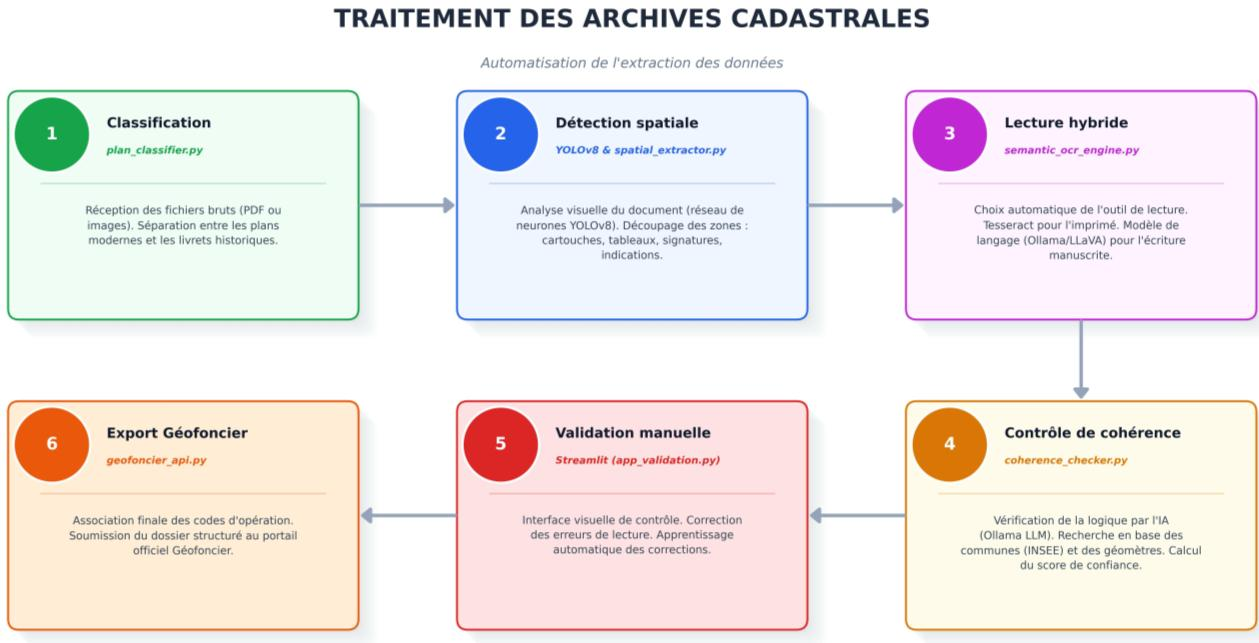
\includegraphics[width=\textwidth]{img/r4p_page2_img1.jpeg}
  \caption{Organigramme des solutions retenues et enchaînement des scripts Python.}
  \label{fig:architecture_pfe}
\end{figure}

Cette séparation en différents scripts permet de dérouler le traitement étape par étape et de modifier plus facilement le code, mais également d'adapter le traitement à de nouveaux cas. La sous-section suivante détaille les outils utilisés et la structure du projet.

\subsection{Environnement technique et organisation du code}

Tout l'outil fonctionne directement sur l'ordinateur du cabinet sous Windows. Aucune donnée n'est envoyée sur Internet, ce qui garantit le respect du secret professionnel évoqué plus tôt.

Les outils et bibliothèques utilisés dans le projet sont les suivants :
\begin{itemize}
  \item PyMuPDF (fitz) : lecture des fichiers PDF créés sur ordinateur (\href{https://github.com/pymupdf/PyMuPDF}{Dépôt PyMuPDF}).
  \item OpenCV et NumPy : nettoyage des images, redressement des lignes et réglage du contraste (\href{https://github.com/opencv/opencv}{Dépôt OpenCV}).
  \item Ultralytics YOLOv8 : repérage et découpage des zones utiles sur la page (\href{https://github.com/ultralytics/ultralytics}{Dépôt YOLOv8}).
  \item PyLaia : lecture de l'écriture manuscrite (\href{https://github.com/jpuigcerver/PyLaia}{Dépôt PyLaia}).
  \item GLiNER : recherche des informations importantes dans le texte (\href{https://github.com/urchade/GLiNER}{Dépôt GLiNER}).
  \item Ollama / LLaVA : modèle de secours en local pour les cas difficiles (\href{https://github.com/ollama/ollama}{Dépôt Ollama}).
  \item Streamlit : création de l'interface de validation (\href{https://github.com/streamlit/streamlit}{Dépôt Streamlit}).
  \item Label Studio : annotation des 500 pages pour l'apprentissage (\href{https://github.com/HumanSignal/label-studio}{Dépôt Label Studio}).
\end{itemize}

Pour garantir la stabilité de l'application et éviter les conflits entre les bibliothèques informatiques, l'ensemble des modules Python s'exécute au sein d'un environnement virtuel dédié. Les dépendances informatiques sont figées dans un fichier de configuration qui recense les versions exactes de chaque paquet. Ce mécanisme permet de réinstaller à l'identique la chaîne de traitement sur n'importe quelle station de travail du cabinet sans risquer de casser la compatibilité du code.

L'arborescence du projet s'organise autour d'un dossier principal regroupant les scripts d'exécution, les fichiers de configuration JSON et les répertoires de données. Les modèles d'intelligence artificielle entraînés (poids YOLOv8 et modèles de lecture) sont stockés dans un dossier spécifique pour séparer la logique du programme des fichiers de paramètres. De même, les fichiers temporaires créés lors du découpage des images sont automatiquement nettoyés en fin de traitement pour ne pas surcharger l'espace disque du serveur local.

Chaque script répond à un rôle précis au sein du flux de travail, facilitant ainsi les évolutions futures.



Pour conserver un code clair et facile à maintenir, les fichiers et scripts du projet sont organisés de la manière suivante :

\begin{small}
\begin{verbatim}
memoire_pfe/
|-- config/                         # Réglages et paramètres (conf.yaml)
|-- Extraction_Archives_Geometre_1/ # Scripts dédiés au 1er fonds d'archives
|-- Extraction_Archives_Geometre_2/ # Scripts dédiés au 2d fonds d'archives
|-- tests/                          # Tests et vérifications automatiques
|-- ex_pdf/                         # Exemples de fichiers PDF de test
|-- plan_classifieur.py              # Tri et classification du document
|-- spatial_extracteur.py            # Découpage visuel par YOLOv8
|-- outil_ocr.py                     # Lecture OCR et extraction de texte
|-- coherence_controle.py            # Contrôle et vérification des données
|-- app_validation.py               # Interface de relecture sous Streamlit
|-- geofoncier_api.py               # Export et envoi vers l'API Géofoncier
+-- main.py                         # Script principal de lancement
\end{verbatim}
\end{small}


Chaque dossier et chaque script a un rôle bien précis dans l'organisation du projet :

\begin{itemize}
  \item \textbf{La configuration et les fichiers de travail} : le dossier \texttt{config/} rassemble les réglages dans un fichier unique (\texttt{conf.yaml}) pour pouvoir modifier les paramètres sans toucher au code. Les dossiers spécifiques par géomètre permettent d'adapter le traitement aux particularités de chaque fonds d'archives. Enfin, les dossiers \texttt{tests/} et \texttt{ex\_pdf/} permettent de valider le programme sur des exemples.
  
  \item \textbf{Les scripts de la chaîne de traitement} : le fichier \texttt{main.py} pilote l'ensemble de la chaîne. Il appelle successivement les scripts de la racine pour trier le document, découper les zones utiles, lire le texte, contrôler la cohérence des données, afficher l'interface de relecture et envoyer les résultats.
\end{itemize}

Les parties suivantes détaillent le rôle de chaque script dans l'ordre du traitement, à commencer par la numérisation des documents.

\subsection{Acquisition, numérisation et correspondance avec les registres}

L'acquisition et la numérisation permettent de convertir les archives papier en fichiers, généralement des PDF. 

Les numérisations sont réalisées directement avec le matériel du cabinet, à savoir le scanner  TOSHIBA e-STUDIO3015AC. Deux résolutions d'acquisition ont été définies selon la nature des pièces :
\begin{itemize}
  \item Une résolution de 300 DPI pour les registres anciens et les documents manuscrits. Cette haute définition a pour but de conserver les détails de l'écriture manuelle et des lignes des tableaux.
  \item Une résolution de 200 DPI pour les plans et pièces imprimées récentes déjà bien lisibles, afin de réduire la taille des fichiers enregistrés sur l'ordinateur.
\end{itemize}

Le fonds traité regroupe des formats de documents variés, allant des grands registres au format A3 jusqu'aux carnets de terrain (non pertinents dans cette étude). De plus, la pose manuelle des feuilles sur la vitre du scanner entraîne souvent de légères rotations des images.

Du fait de cette problématique, un script Python a été développé pour l'acquisition. Il permet de séparer automatiquement la vue double en deux images distinctes, d'ajuster les marges extérieures et d'attribuer une numérotation propre à chaque page.


\subsection{Classification et orientation du document}

Le tri permet de savoir quel type de document est à traiter (plan récent fait sur ordinateur, plan ancien scanné, registre manuscrit ou document imprimé), et orienter le traitement en conséquence, vers la bonne branche du programme. Pour gagner du temps, le script \texttt{plan\_classifieur.py} utilise des règles simples qui s'exécutent en quelques secondes.

Le choix repose sur trois critères :

\begin{itemize}
  \item Présence de texte informatique : Si le fichier est un PDF issu d'un logiciel de dessin, son texte est déjà lisible. La bibliothèque \texttt{PyMuPDF} le détecte directement. Ces fichiers évitent le traitement d'image et passent tout de suite à la lecture du texte.
  
  \item Résolution de l'image (DPI) : La résolution du fichier est lue. En dessous de 150 DPI, le document est ancien ou de faible qualité et demande un nettoyage d'image.
  
  \item Quantité d'encre sur la page : Le système compte la proportion de pixels noirs. Sur un plan, l'encre occupe moins de 5 \% de la feuille. Sur un registre écrit à la main, cette proportion monte entre 15 \% et 20 \% à cause du texte et des remarques.
\end{itemize}

En cas de doute, le document est envoyé vers la lecture manuscrite. Un modèle capable de lire le manuscrit sait aussi lire le texte imprimé, alors qu'un OCR classique échoue sur l'écriture manuelle.

\subsection{Segmentation visuelle par YOLOv8}

Envoyer une page entière vers le modèle de lecture cause des erreurs, car une page contient des ratures, des tampons et des notes.

Il est donc nécessaire d'isoler les zones utiles avant la lecture. Le script \texttt{spatial\allowbreak\_extracteur\allowbreak.py} s'appuie sur le modèle pré-entraîné YOLOv8 (\texttt{yolov8n.pt}) pour découper directement les régions d'intérêt sur la page (cartouches DMPC, blocs de texte, tableaux de parcelles, tampons des géomètres).

L'utilisation  de ce modèle pré-entraîné permet d'identifier les boîtes englobantes sans nécessiter une phase d'entraînement. L'algorithme NMS (présenté au chapitre~\ref{sec:etat_art}) supprime les encadrements doubles pour ne conserver que la boîte ayant le meilleur score de confiance. Ces boites peuvent être observées sur la figure \ref{fig:nms_exemple}.

\begin{figure}[H]
  \centering
  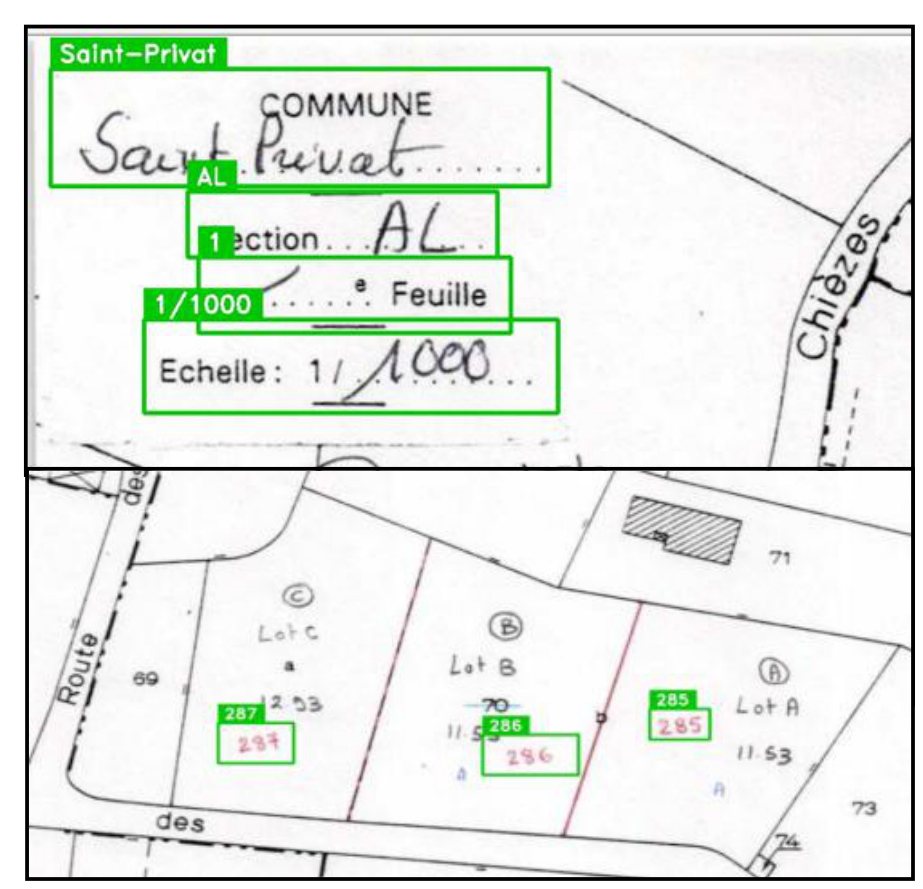
\includegraphics[width=0.6\textwidth]{img/r4p_fig2_tight.png}
  \caption{Zones de détection et affichage des boîtes englobantes sur un document d'arpentage (DMPC) par YOLOv8.}
  \label{fig:nms_exemple}
\end{figure}

Comme le montre ce résultat, YOLOv8 parvient à repérer les informations essentielles du document d'arpentage (DMPC) en traçant un cadre vert autour de chaque élément utile : le nom de la commune, la section cadastrale, le numéro de feuille et l'échelle du plan. Ces zones découpées sont ensuite transmises aux scripts de lecture pour extraire proprement le texte de chaque case.


% A RELIRE
\subsection{Prétraitement de l'image}

Envoyer un extrait d'image directement vers le moteur de lecture peut causer des erreurs si le document a été posé de travers ou si le papier est dégradé. Plusieurs traitements d'image sont appliqués avant la lecture.

Lorsqu'une feuille est numérisée avec un léger penchant, les lignes de texte ne sont plus horizontales, ce qui perturbe la lecture mot à mot. Pour corriger cela, le script applique une chaîne de traitement classique. Le filtre de Canny~\citep{canny_edge_1986} détecte d'abord les contours de l'image en mesurant les variations locales de luminosité, puis la transformée de Hough~\citep{duda_hough_1972} analyse l'espace des paramètres $(\rho, \theta)$ pour trouver les lignes les mieux représentées dans l'image :

\begin{equation}
  \rho = x \cos\theta + y \sin\theta
\end{equation}

où $\rho$ est la distance de la droite à l'origine et $\theta$ son angle par rapport à l'axe horizontal. Les lignes les plus représentées correspondent aux séparateurs de colonnes ou aux lignes de texte du document. L'angle dominant $\theta$ déduit de ces calculs définit l'inclinaison à corriger. Le script applique ensuite une rotation inverse de cet angle sur toute l'image avant de la transmettre au modèle de lecture.

Comme présenté dans l'état de l'art (section~\ref{subsec:ocr}), les archives présentent souvent du papier jauni, des taches ou de l'encre effacée. Un réglage global du contraste sur toute la page risque de faire disparaître les écritures claires sur fond clair. Le script utilise donc la méthode de binarisation par seuil local d'~\citet{otsu_threshold_1979}. L'image est découpée en fenêtres rectangulaires qui se chevauchent partiellement, et l'algorithme calcule automatiquement le seuil de séparation optimal entre l'écriture et le fond pour chaque région. Ce seuil est déterminé en maximisant la variance inter-classes :

\begin{equation}
  \sigma_B^2 = \omega_0(t)\,\omega_1(t)\,\bigl[\mu_0(t) - \mu_1(t)\bigr]^2
\end{equation}

où $\omega_0$ et $\omega_1$ sont les poids de probabilité des deux classes (fond et encre) et $\mu_0$, $\mu_1$ leurs moyennes d'intensité pour un seuil $t$ donné. Maximiser cette variance permet de séparer les deux classes de pixels, même quand leur niveau de gris varie d'une zone à l'autre du document. Cette adaptation locale fait ressortir l'écriture manuscrite et les traits légers tout en éliminant les variations de couleur dues au vieillissement du papier.

Certains documents anciens, numérisés depuis un livre ou un carnet relié, présentent une déformation en trapèze vers l'intérieur de la reliure. Dans ce cas, la simple rotation ne suffit pas à redresser les lignes de texte. Pour les détections de boîtes englobantes inclinées par YOLOv8, le script applique une transformation de perspective (homographie) qui reprend les quatre coins du cadre détecté et les projette sur un rectangle à plat via la fonction \texttt{cv2.getPerspectiveTransform} d'OpenCV :

\begin{equation}
  \begin{pmatrix} x' \\ y' \\ 1 \end{pmatrix} = H \begin{pmatrix} x \\ y \\ 1 \end{pmatrix}, \quad H \in \mathbb{R}^{3\times3}
\end{equation}

Cette correction garantit que la zone extraite est présentée au moteur de lecture sous un format plat et normalisé, quel que soit l'angle ou la déformation d'origine du document.

La Figure~\ref{fig:pretraitement_exemple} illustre le résultat de ces étapes de correction d'image.

\begin{figure}[H]
  \centering
  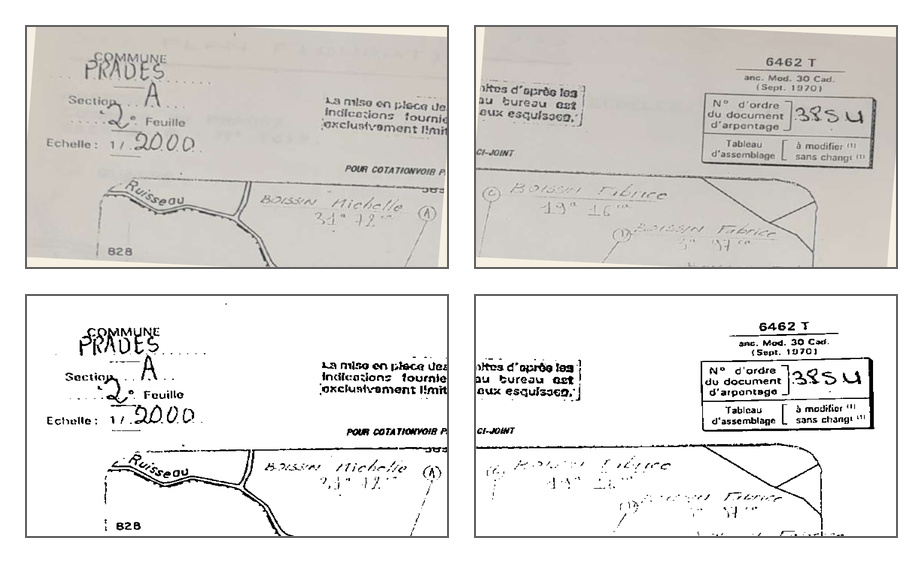
\includegraphics[width=0.85\textwidth]{img/pretraitement_vrai_plan.png}
  \caption{Zoom sur les cartouches d'un document : comparaison entre l'image numérisée inclinée à -3,5\textdegree{} (en haut) et le résultat droit après seuillage d'Otsu (en bas). L'image a volontairement été mal scannée pour les besoins de l'écrit.}
  \label{fig:pretraitement_exemple}
\end{figure}

Sur l'image brute en haut, l'inclinaison de la feuille rend la lecture des lignes difficile. Après le passage des filtres en bas, le texte est remis droit et les écritures ressortent en noir sur un fond blanc. Ce nettoyage facilite le travail du moteur de lecture.

En complément du redressement et de la binarisation, une opération de filtrage morphologique est appliquée pour éliminer les petits bruits d'encre et les bavures. Une fermeture morphologique (dilatation suivie d'une érosion par un élément structurant rectangulaire) permet de relier les traits discontinus des caractères manuscrits effacés tout en supprimant les points isolés. De plus, un rognage automatique supprime les marges noires du scanner en repérant les bords du papier, ce qui évite d'envoyer des bordures sombres inutilement aux modèles de segmentation.
% >>>>>>>>>>>>>>>>>>>




\subsection{Extraction du texte et des données clés}

Une fois les zones du document recadrées et nettoyées par le prétraitement, l'étape de lecture s'exécute via le script \texttt{outil\_ocr.py}. Cette phase contient deux approches  selon le texte du document:
\begin{itemize}
  \item Le moteur Tesseract traite les caractères tapés. Il convertit les zones imprimées en chaînes de texte.
  \item Le modèle PyLaia prend le relais pour l'écriture manuscrite. Il lit les mots lettre par lettre.
\end{itemize}

Le texte brut extrait par l'OCR contient toutefois des phrases entières, des abréviations ou du bruit entourant l'information recherchée. Pour extraire les données utiles sans écrire des dizaines de règles, l'outil s'appuie sur le modèle de reconnaissance d'entités GLiNER.

Ce dernier analyse directement la chaîne de texte brute et y recherche les champs cibles (le nom de la commune, le numéro de dossier, la section cadastrale, la date et le nom du géomètre). Pour chaque champ extrait, le modèle attribue une note de confiance comprise entre 0 et 1 :
\begin{itemize}
  \item Si le score de confiance est supérieur ou égal au seuil défini (réglé à 0,45), l'information est considérée comme fiable et pré-remplie automatiquement.
  \item Si le score de confiance est inférieur à 0,45 (dû à une tache, une écriture difficile ou une rature), l'entité est marquée comme douteuse et transférée à l'étape suivante d'arbitrage.
\end{itemize}

Ce score de confiance ne repose pas uniquement sur la probabilité calculée par le modèle GLiNER. Le script de contrôle (\texttt{coherence\_controle.py}) vient aussi vérifier la cohérence des réponses. Par exemple, si la commune trouvée existe bien dans la base de données de l'Ardèche (\texttt{ardeche.json}) et que le format de la section est correct, la note globale reste élevée. En revanche, si une lecture est étrange ou que le format ne correspond pas, le score baisse en dessous de 0,45 pour demander une confirmation par le modèle suivant.


La Figure~\ref{fig:extraction_ocr_gliner} illustre l'exécution de l'outil sur un document de type DA.

\begin{figure}[H]
  \centering
  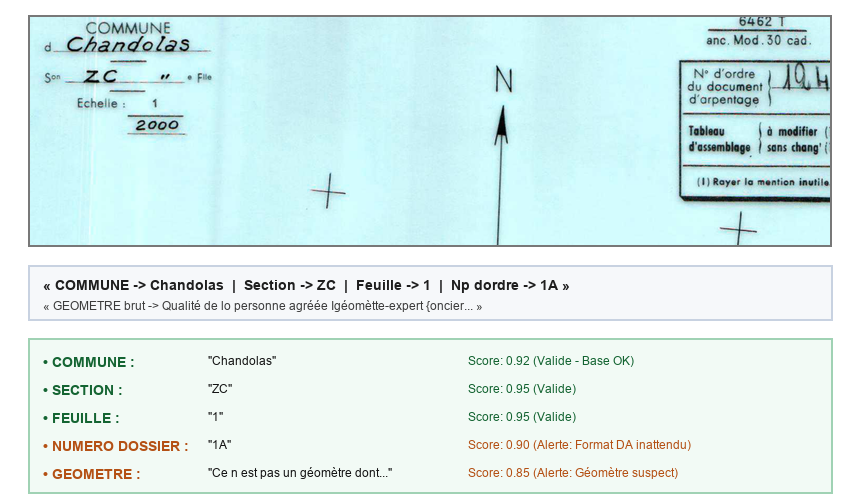
\includegraphics[width=0.9\textwidth]{img/extraction_ocr_gliner.png}
  \caption{Processus d'extraction des entités par GLiNER.} 
  \label{fig:extraction_ocr_gliner}
\end{figure}

En haut de l'image, le script découpe d'abord la zone d'intérêt du cartouche. Au milieu, le moteur de lecture extrait la chaîne de texte brute, avec ses fautes d'impression ou ses abréviations. Enfin, en bas, GLiNER et le script de vérification classent les informations dans les bons champs en leur attribuant une note de confiance et des alertes si une donnée semble fausse, l'envoyant dans ce cas à l'étape suivante d'arbitrage.

Lorsque le document contient plusieurs lignes de texte proches (par exemple dans le tableau des parcelles ou dans l'en-tête du procès-verbal), la simple extraction linéaire des mots ne suffit pas. Le script calcule le rectangle englobant de chaque mot reconnu et regroupe les termes appartenant à une même ligne selon leur chevauchement vertical. Les paires clé-valeur (comme la mention "Commune de" suivie du nom de la localité) sont associées en mesurant la distance horizontale minimale entre le libellé imprimé et la réponse manuscrite.

Pour éviter que des mots communs du vocabulaire juridique ou topographique (tels que "voie", "chemin", "parcelle", "section") ne soient interprétés à tort comme des noms de personnes ou de lieux, les réponses proposées par le modèle d'entités sont filtrées par un dictionnaire de mots exclus. Seules les entités qui passent ce filtre et qui présentent une similarité suffisante avec les référentiels régionaux sont conservées avec un score de confiance supérieur au seuil de validation.

Cette combinaison d'outils permet de traiter l'ensemble des cas d'usage sans imposer de réentraînement lourd sur chaque nouveau type de document. Comme nous l'étudierons lors de la présentation de l'interface de validation au chapitre~\ref{sec:fiabilisation}, la note de confiance attribuée à chaque champ détermine la couleur du badge affiché à l'écran, guidant ainsi l'opérateur vers les champs nécessitant une vérification prioritaire.





\subsection{Arbitrage par modèle VLM}

Le traitement par modèle VLM demande plus de temps de calcul (10 à 30 secondes par zone d'image). Il est donc réservé uniquement aux cas où la première lecture par l'OCR ou GLiNER reste incertaine (score de confiance inférieur à 0,45 ou alerte de cohérence).

Le modèle VLM \texttt{llava} tourne alors sur la machine via l'outil Ollama (port 11434). Les images ne quittent ainsi jamais l'ordinateur.

Contrairement à l'OCR qui lit le texte caractère par caractère, le modèle VLM regarde l'image de la zone dans son ensemble et répond à une consigne écrite. Par exemple, pour valider la commune, la consigne configurée dans le script est la suivante :

\begin{quote}
\textit{« Quel est le nom de la commune d'Ardèche écrit dans cette case ? Réponds uniquement par le nom de la commune, sans phrase, et répond par INCERTAIN lorsque tu n'arrive pas à une réponse plausible. »}
\end{quote}

Si le modèle parvient à lire la zone, il met à jour la valeur. S'il hésite, il répond « INCERTAIN », ce qui signale le dossier pour la vérification humaine.

La Figure~\ref{fig:ollama_vlm_schema} montre cet arbitrage sur un document issu du fonds du Géomètre B (\texttt{EXEMPLE\_}\linebreak[0]\texttt{GEOMETRE\_}\linebreak[0]\texttt{B.pdf}). L'OCR brut lit la chaîne manuscrite (\texttt{St Didier suus Aubenas}) et retient initialement la commune d'Aubenas. Le script de contrôle détecte alors une alerte de cohérence, due à une longueur anormale de caractères, ce qui déclenche automatiquement le modèle VLM. Ce dernier réexamine la zone et valide la commune exacte de Saint-Didier-sous-Aubenas.



\begin{figure}[H]
  \centering
  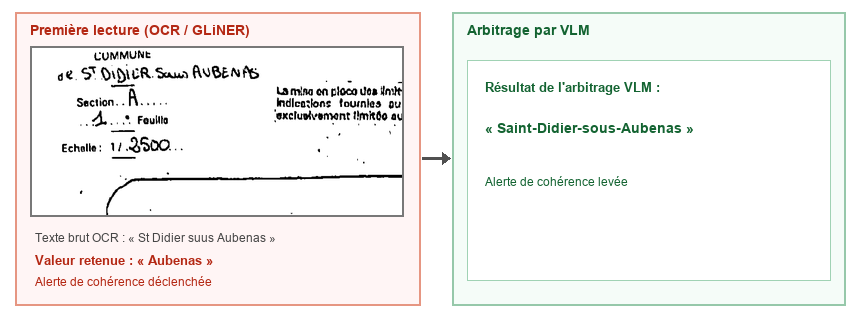
\includegraphics[width=0.95\textwidth]{img/vlm_arbitrage_exemple.png}
  \caption{Arbitrage par le modèle VLM déclenché par une alerte de cohérence sur le document du Géomètre B (\texttt{EXEMPLE\_GEOMETRE\_B.pdf}).}
  \label{fig:ollama_vlm_schema}
\end{figure}

En plus des communes, le modèle VLM est utilisé pour d'autres cas sur les documents :

\begin{itemize}
  \item Pour les choix pré-imprimés sur un DMPC, afin d'identifier l'option A, B ou C non rayée au stylo, une information qui peut être utile pour un opérateur.
  \item Pour les dates ou les jours impossibles renvoyés par la première lecture.
  \item Pour lire le texte sous les tampons ou les pliures, par exemple pour détecter le nom du géomètre-expert ayant effectué la mission.
  \item Pour les noms de propriétaires, où il est fréquemment utilisé car ils sont écrits à la main et qu'aucune règle ne permet de les identifier avec certitude.
\end{itemize}

L'utilisation de consignes textuelles ciblées permet d'adapter la sensibilité du modèle VLM selon la nature du champ. Pour réduire le temps de réponse et éviter que le modèle ne génère des phrases trop longues, la température de génération est réglée à une valeur très faible (0,1). Cette contrainte force le modèle à retourner des réponses concises et directes, immédiatement nettoyées par une fonction de filtrage qui supprime la ponctuation inutile et met en majuscules le texte extrait avant sa validation.

En cas d'échec de réponse du modèle VLM ou si le temps de calcul dépasse un seuil tolérable de 45 secondes, l'arbitrage est interrompu et la mention par défaut est attribuée au champ, pour que l'opérateur effectue lui-même la vérification dans l'interface web.

Comme indiqué lors de la présentation théorique des VLM (section~\ref{sec:vlm_execution}), cette exécution en local via l'outil Ollama garantit l'autonomie complète du cabinet sans transmettre d'images sur des serveurs externes.


\subsection{Formats de données, règles de contrôle et bilan}

Le résultat de l'extraction est enregistré sous la forme d'un fichier JSON structuré, associé à chaque document. Ce fichier regroupe l'ensemble des valeurs lues, leurs scores de confiance respectifs et les alertes générées par le contrôle de cohérence.

Pour s'assurer qu'aucune information absurde ne soit transmise à l'étape suivante, le script \texttt{coherence\_controle.py} applique une série de vérifications automatiques :

\begin{itemize}
  \item Vérification des communes : le nom extrait est comparé à la liste officielle des communes de l'Ardèche et de la Drôme (via le Code Officiel Géographique de l'INSEE). Si l'orthographe s'écarte du nom de référence, la distance de Levenshtein calcule la commune la plus proche. Si le score de correspondance est inférieur à un seuil défini (88\,\%), le champ est marqué en alerte.
  \item Cohérence temporelle : la date de l'acte doit être comprise dans une plage plausible (par exemple entre 1950 et l'année en cours). Une date située en dehors de cette plage déclenche une alerte de validation.
  \item Format des références : les numéros de dossiers et les références cadastrales sont contrôlés par des expressions régulières (regex) pour vérifier leur structure (par exemple, une section cadastrale composée de 1 ou 2 lettres, suivie d'un numéro de parcelle entier).
\end{itemize}

Ce schéma de données structuré permet de conserver la traçabilité complète de chaque extrait. Comme nous le verrons lors de la phase d'exportation vers Géofoncier (chapitre~\ref{sec:integration}), ce fichier JSON sert de socle pour construire la requête REST transmise à l'API.


À la fin de ce processus, toutes les informations contrôlées sont enregistrées dans un fichier JSON propre pour chaque document.

Même si le système automatise la majorité du travail de lecture, des erreurs peuvent persister : une information est parfois illisible, sujette à interprétation, ou simplement hors de portée des modèles. Un contrôle humain est alors nécessaire. Le chapitre suivant présente la partie fiabilisation et l'interface graphique permettant à l'utilisateur de contrôler et valider les dossiers avant l'envoi final sur Géofoncier.


\subsection{Constitution du jeu de données d'entraînement}

Le modèle YOLOv8 utilisé pour découper les zones d'intérêt sur les pages de documents doit être entraîné sur des exemples issus du fonds du cabinet. Un modèle pré-entraîné sur des images génériques est incapable de localiser correctement des zones aussi spécifiques que le cartouche d'un DMPC ou le tableau de parcelles d'un DA.

Pour constituer ce jeu d'entraînement, 500 pages ont été sélectionnées parmi les fonds des deux géomètres. La sélection couvre plusieurs générations de formulaires (avant et après 1980), plusieurs niveaux de qualité de numérisation (200 à 300 DPI), plusieurs types d'actes (DMPC, DA, PV de bornage) et plusieurs états de conservation (papier propre, papier jauni, tampon en marge, rature). Cette diversité est indispensable pour que le modèle apprenne à détecter les zones dans des conditions variables et ne soit pas limité aux seuls documents en parfait état.

Les 500 pages ont été annotées manuellement à l'aide du logiciel libre Label Studio, installé en local sur la machine du cabinet. Label Studio permet de tracer des boîtes englobantes sur des images et d'associer une étiquette à chaque zone. Les classes définies pour ce projet sont les suivantes : \texttt{commune}, \texttt{section}, \texttt{parcelles}, \texttt{date}, \texttt{geometre} et \texttt{tampon}.



Chaque page a été annotée par une seule personne et vérifiée par une seconde lors d'une phase de relecture. Les boîtes ont été tracées au plus près du contenu, sans inclure les marges extérieures du formulaire. Au total, environ 3\,200 boîtes englobantes ont été produites sur les 500 pages, soit une moyenne de 6,4 zones annotées par page.

Les 500 images annotées ont été réparties en trois sous-ensembles : 70\,\% pour l'entraînement (350 images), 15\,\% pour la validation (75 images) et 15\,\% pour le test final (75 images). L'entraînement a été réalisé sur 50 époques avec le modèle léger \texttt{yolov8n.pt}, ce qui prend environ 40 minutes sur la carte graphique NVIDIA du poste de travail. Le score de détection moyen atteint sur le jeu de test est de mAP50 = 0,94, ce qui signifie que le modèle localise correctement 94\,\% des zones avec un seuil de chevauchement de 50\,\%.

Le système est conçu pour être ré-entraînable sans intervention technique complexe. Chaque fois qu'un lot de nouveaux documents est annoté, le script de ré-entraînement peut être relancé depuis un fichier de commandes qui exporte les annotations et démarre l'entraînement. Le modèle mis à jour remplace automatiquement l'ancien sans modifier le reste du code.


\subsection{Gestion des exceptions et stratégies de repli}

Dans une chaîne de traitement automatisée traitant des documents numérisés aux formats variés, des erreurs de calcul ou des échecs de détection peuvent survenir à chaque étape. Pour éviter qu'un fichier défectueux ne bloque l'ensemble du traitement par lot, le script principal intègre une gestion des exceptions associant des stratégies de repli.

Si le modèle YOLOv8 ne retourne aucune boîte englobante sur une page (par exemple en cas de document au format non standard ou très sombre), le script bascule automatiquement sur un découpage géométrique par défaut. Les coordonnées des zones sont calculées à partir de ratios fixes (cartouche supérieur droit entre 0\,\% et 25\,\% de la hauteur, tableau central entre 25\,\% et 75\,\% de la hauteur). Un avertissement est inscrit dans le fichier JSON pour signaler le recours au découpage par défaut.

Si la carte graphique est sollicitée par une autre application ou si la mémoire vidéo est insuffisante lors du chargement des modèles PyLaia ou GLiNER, le système bascule automatiquement l'exécution du modèle concerné sur le processeur central (CPU). Le temps de calcul s'allonge, mais le traitement continue sans interruption.

Lorsque l'OCR extrait des chaînes de caractères contenant des octets invalides ou des symboles non imprimables (fréquent sur les tampons baveux), la fonction de nettoyage filtre les caractères hors de la plage UTF-8 standard. Si la chaîne nettoyée est vide, le champ prend la valeur \texttt{INCERTAIN} et le score de confiance est mis à 0, ce qui signale le dossier pour la relecture dans l'interface Streamlit (chapitre~\ref{sec:fiabilisation}).

Le Tableau~\ref{tab:strategies_repli} récapitule les principales exceptions gérées par l'architecture et les réponses apportées.

\begin{table}[H]
  \centering
  \caption{Synthèse des exceptions gérées par la chaîne de traitement et mécanismes de repli.}
  \label{tab:strategies_repli}
  \small
  \begin{tabular}{p{4.5cm} p{4.5cm} p{5.5cm}}
    \toprule
    \textbf{Événement déclencheur} & \textbf{Détection / Exception} & \textbf{Stratégie de repli appliquée} \\
    \midrule
    Aucune boîte YOLO trouvée & Liste de boîtes vide & Découpage géométrique par ratios de page. \\
    Mémoire GPU insuffisante & Exception mémoire CUDA & Bascule automatique de l'inférence sur CPU. \\
    Texte OCR illisible ou vide & Chaîne vide après nettoyage & Champ marqué \texttt{INCERTAIN}, alerte dans l'IHM. \\
    Fichier PDF corrompu & Erreur de lecture fichier & Document déplacé dans \texttt{errors/}, log d'échec. \\
    API Géofoncier indisponible & Erreur de connexion réseau & Stockage du dictionnaire dans \texttt{pending\_api/}. \\
    \bottomrule
  \end{tabular}
\end{table}

Cette organisation garantit la robustesse de l'application sur de grands volumes de fichiers. Un document comportant une anomalie est isolé sans interrompre le traitement des autres pièces du lot.

De plus, l'ensemble des événements et erreurs survenus lors de l'exécution est consigné dans un fichier de journalisation quotidien (\texttt{traitement.log}). Ce journal d'erreurs indique l'horodatage précis, le nom du fichier concerné, le module informatique à l'origine de l'alerte ainsi que le code de l'erreur. Cette traçabilité permet au responsable informatique du cabinet d'identifier rapidement les documents problématiques et d'ajuster les règles de repli si nécessaire.
% >>>>>>>>>>>>>>>>>>>










\clearpage
% !TeX root = main.tex

\section{Validation des données et interface utilisateur}
\label{sec:fiabilisation}

Ce chapitre présente la phase de validation des données extraites automatiquement et l'interface développée pour les opérateurs du cabinet. Il détaille le fonctionnement de l'application Streamlit, la gestion de l'état en mémoire, les règles de contrôle de cohérence, ainsi que les outils de recherche et de géolocalisation nécessaires avant l'exportation vers Géofoncier.


\subsection{Principes et fonctionnement de l'application Streamlit}

Le traitement des archives présenté au chapitre précédent produit des résultats sur la grande majorité des documents. Cependant, il est impossible de s'en remettre entièrement à ce type de détection pour verser des données sur un portail national à but juridique. Les informations extraites alimentent le Référentiel Foncier Unifié (RFU) de Géofoncier. Une erreur sur le nom d'une commune, sur la section cadastrale ou sur le numéro d'un dossier génère une pastille pouvant être mal localisée, voire une fiche indexée sous le mauvais acte foncier. Compte tenu de la valeur juridique de ces documents, ce type d'erreur n'est pas tolérable.

L'OCR produit parfois des chaînes de caractères incorrectes car la source même de la donnée peut être dégradée, et le modèle VLM retourne la mention \texttt{INCERTAIN} lorsqu'il ne parvient pas à trouver une réponse. Dans tous ces cas de figure, seule une vérification humaine valide la donnée. L'interface de validation assiste l'opérateur en lui présentant le document et les données extraites côte à côte, en lui signalant les champs soumis à un doute, et en lui fournissant des outils de recherche dans les répertoires existants. Une fois un dossier confirmé par l'opérateur, le fichier CSV correspondant est mis à jour et les données peuvent être transmises à l'API Géofoncier.

L'application est développée en Python avec le framework Streamlit, qui permet de créer des applications web sans écrire de code HTML. Elle s'exécute localement sur la machine du cabinet, accessible depuis n'importe quel navigateur web du réseau local sur le port 8501. Les données restent ainsi confinées au réseau du cabinet, sans transiter par des serveurs externes.

Pour bien comprendre la conception de l'application, il faut prendre en compte le fonctionnement de Streamlit. À chaque fois que l'utilisateur interagit avec l'application (en cliquant sur un bouton ou en modifiant une case), le script Python est intégralement réexécuté du début à la fin. Ce procédé réinitialise la page et effacerait les corrections saisies avant qu'elles ne soient sauvegardées. Pour éviter ce problème, l'application conserve les modifications en cours dans une mémoire temporaire gérée par la session. Les données modifiées y sont stockées et restent affichées à l'écran tout au long de la relecture du document. La sauvegarde définitive n'intervient que lorsque l'opérateur clique sur le bouton de validation.

La gestion de cette mémoire de session s'organise autour de plusieurs variables conservées d'une exécution à l'autre :
\begin{itemize}
  \item \textbf{L'index du document} : conserve la position du document actuellement affiché dans le lot de travail sélectionné.
  \item \textbf{Les valeurs du document} : mémorisent l'ensemble des données des champs d'indexation (commune, section, date, géomètre, parcelles) et mettent à jour les champs en temps réel dès qu'une modification est saisie.
  \item \textbf{Les indicateurs de confiance} : conservent les scores d'exactitude et les alertes associées à chaque champ pour adapter la couleur des badges visuels.
  \item \textbf{L'historique local des corrections} : enregistre les paires de valeurs corrigées pour proposer des suggestions automatiques si la même erreur survient sur d'autres pièces du même lot.
\end{itemize}

Grâce à cette architecture, l'opérateur peut naviguer dans le document, ajuster le zoom de l'image scannée et modifier plusieurs champs sans subir de réinitialisation impromptue des saisies.





\subsection{Structure de l'interface et formulaire de correction}

L'écran principal de l'application (Figure~\ref{fig:interface_haut}) s'ouvre sur un en-tête intitulé \enquote{Validation des archives cadastrales}. Dans la barre supérieure, l'opérateur choisit son fichier de travail dans le menu déroulant \enquote{Fichier de travail}, consulte l'identifiant du document chargé (par exemple \texttt{07110\_000\_160} pour la commune de Joyeuse), ainsi que le compteur de progression du lot en cours (\texttt{0 / 1 documents validés}).

L'espace de travail est structuré en deux colonnes principales :
\begin{itemize}
  \item La colonne de gauche, intitulée \enquote{SAISIE \& CORRECTION}, regroupe l'ensemble des champs d'indexation sous la forme d'un formulaire interactif organisé par groupes (\textit{Localisation}, \textit{Références \& Acte}, \textit{Intervenants}, et \textit{Parcelles}).
  \item La colonne de droite, intitulée \enquote{APERÇU DU DOCUMENT (ZOOM INTERACTIF)}, affiche l'image scannée du plan cadastral.
\end{itemize}

\begin{figure}[H]
  \centering
  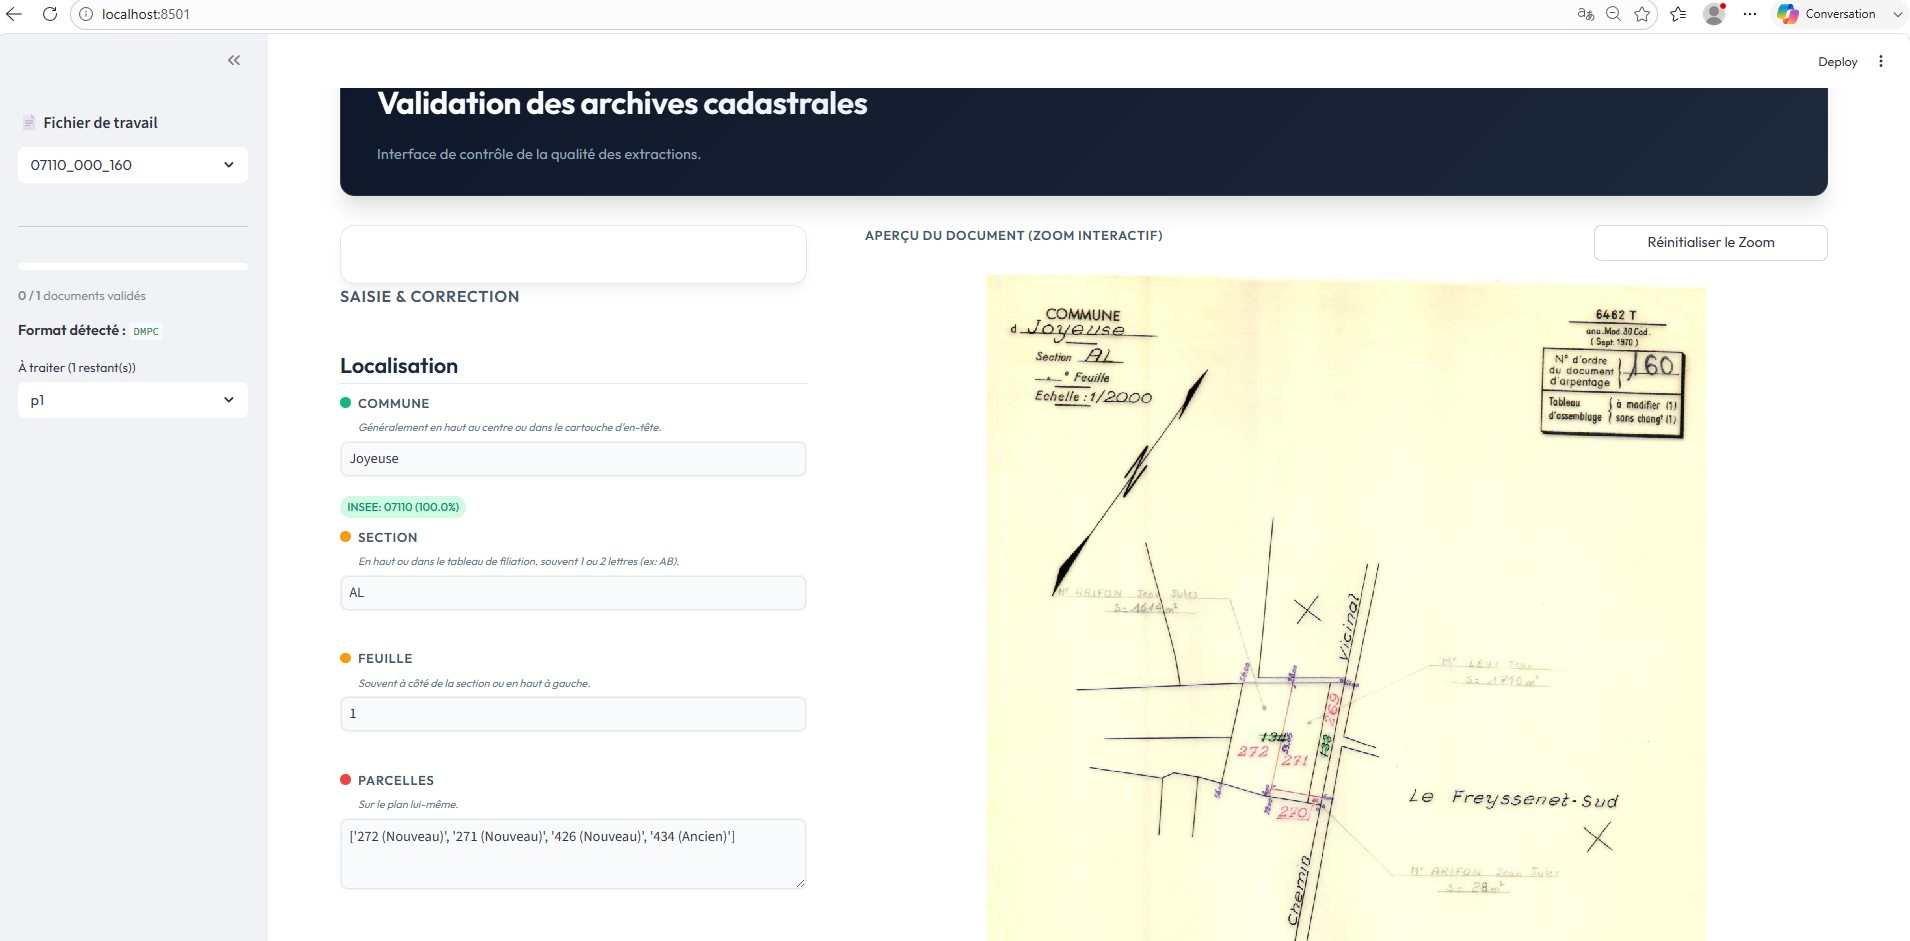
\includegraphics[width=1\textwidth]{img/interface_haut.jpg}
  \caption{Partie supérieure de l'interface de validation, montrant l'en-tête, le sélecteur de fichier, l'identifiant du document \texttt{07110\_000\_160} et la disposition en deux colonnes.}
  \label{fig:interface_haut}
\end{figure}

La colonne de gauche regroupe les champs à vérifier sous la forme d'une liste d'éléments organisés en plusieurs groupes (\textit{Localisation}, \textit{Références \& acte}, \textit{Intervenants}, et \textit{Parcelles}). Pour chaque champ, l'interface affiche la valeur extraite et une couleur indiquant le niveau de confiance.

Comme l'illustre l'extrait de la Figure~\ref{fig:zoom_commune}, le champ \texttt{COMMUNE} affiche la valeur extraite \texttt{Joyeuse} accompagnée du code \texttt{INSEE: 07110 (100.0\%)}, qui confirme la correspondance avec le référentiel des communes.

\begin{figure}[H]
  \centering
  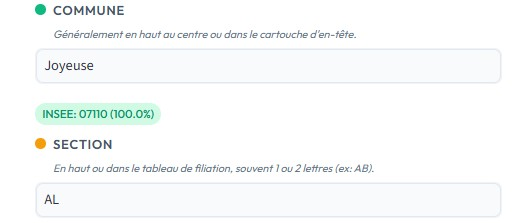
\includegraphics[width=0.65\textwidth]{img/zoom_commune.jpg}
  \caption{Extrait du formulaire de correction montrant le champ Commune .}
  \label{fig:zoom_commune}
\end{figure}

Dans la colonne de droite, un outil de navigation permet de zoomer sur le document et de se déplacer dans l'image pour examiner les champs. Un bouton \enquote{Réinitialiser le Zoom} placé au-dessus de l'image permet de réinitialiser l'affichage à tout moment.


Quand l'opérateur modifie une valeur dans le document, l'application applique une normalisation automatique : mise en majuscules de la section, formatage de la date en \texttt{JJ/MM/AAAA}, nettoyage des séparateurs de parcelles et résolution du code INSEE via la base de données des communes.

L'application mémorise également les corrections apportées par l'opérateur. Quand il corrige un champ (commune, géomètre, section, nature de l'acte...), la correspondance entre la valeur extraite et la valeur corrigée est sauvegardée. Sur les documents suivants du même fonds, si l'application retrouve la même valeur erronée, elle la remplace automatiquement, et affiche un badge \enquote{Auto-corrigé} à côté du champ pour le signaler. Concrètement, une erreur répétée, comme un nom de commune systématiquement mal lu, n'a besoin d'être corrigée qu'une seule fois pour tout une série de scans.


\subsection{Recherche dans les répertoires et géolocalisation}

Une fois les champs validés, l'interface bascule sur un second écran organisé en trois étapes.

Pour retrouver le numéro de dossier original dans les répertoires du cabinet, l'opérateur utilise d'abord le formulaire de recherche (Figure~\ref{fig:etape1_recherche}). Ce formulaire comporte quatre champs : commune, section cadastrale, numéro de parcelle et année. Les valeurs pré-remplies proviennent de l'étape de détection automatique (chapitre~\ref{sec:architecture}), mais l'opérateur peut les ajuster en cas d'erreur. Un clic sur le bouton \enquote{Rechercher dans le répertoire} interroge le fichier du géomètre concerné, en s'appuyant sur les identifiants cadastraux ou sur les noms de propriétaires. 

\begin{figure}[H]
  \centering
  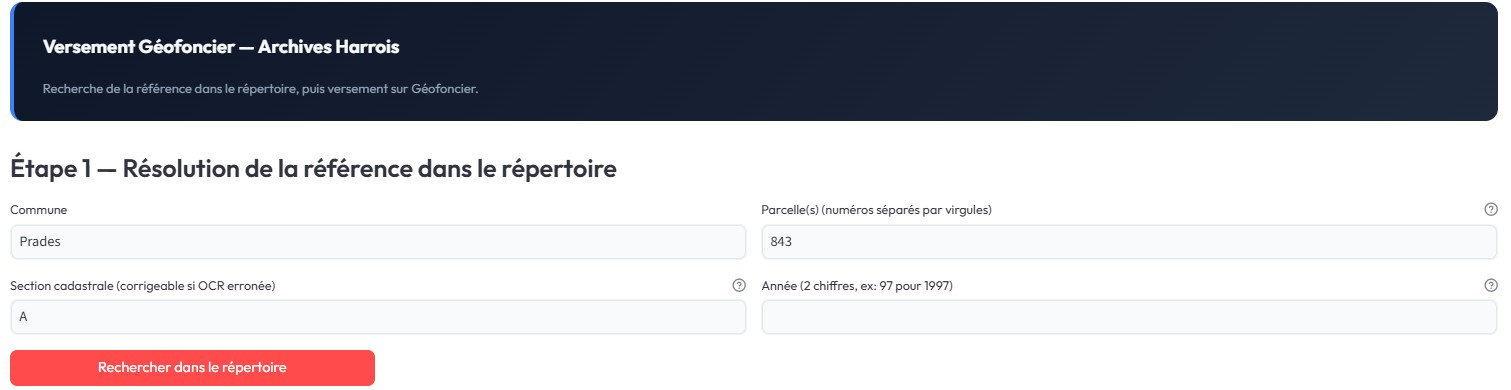
\includegraphics[width=0.85\textwidth]{img/Etape 1_recherche_reference.jpg}
  \caption{Étape 1 -- Formulaire de recherche et de résolution de la référence dans le répertoire.}
  \label{fig:etape1_recherche}
\end{figure}

Lorsque la recherche donne une correspondance unique, celle-ci est directement affichée et validée dans un encadré vert. En revanche, si plusieurs dossiers correspondent aux critères saisis, l'application présente un tableau de choix permettant à l'opérateur de sélectionner la référence exacte avant de poursuivre.

\begin{figure}[H]
  \centering
  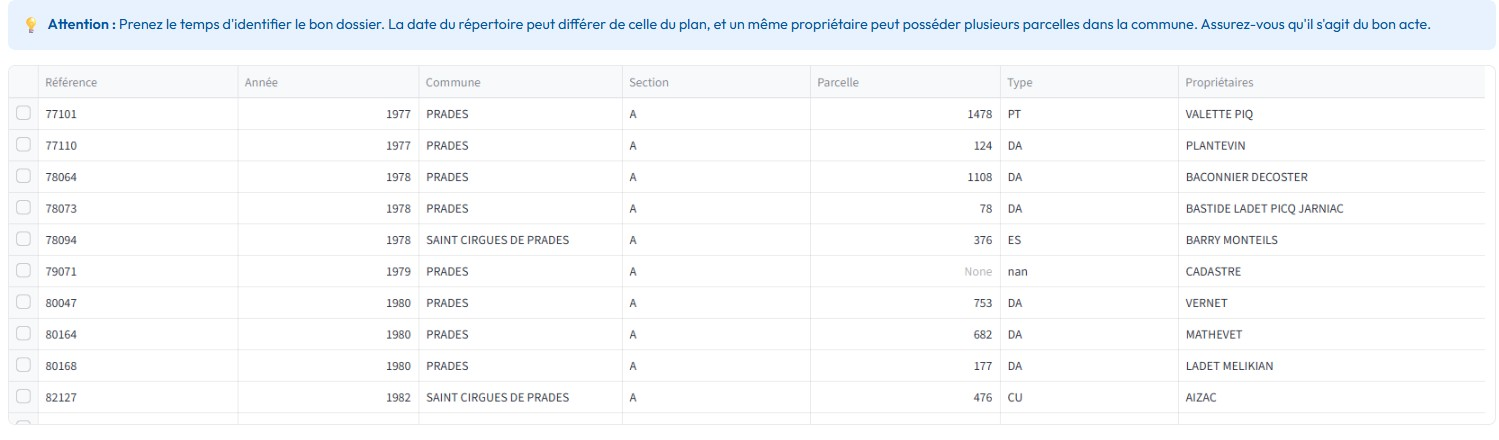
\includegraphics[width=0.85\textwidth]{img/etape_1_liste_possibilites.jpg}
  \caption{Étape 1 -- Tableau de sélection parmi plusieurs dossiers candidats en cas d'ambiguïté.}
  \label{fig:etape1_candidats}
\end{figure}

Comme illustré Figure~\ref{fig:etape1_candidats}, l'opérateur doit trancher manuellement en s'appuyant sur les informations disponibles dans le tableau. L'année de l'acte et les noms des propriétaires sont généralement les éléments les plus fiables pour identifier le bon dossier, notamment lorsque plusieurs opérations portent sur la même parcelle.

Une fois la référence du dossier confirmée, l'interface passe automatiquement à la phase de localisation cartographique.

L'étape suivante s'appuie sur une carte interactive intégrée via la bibliothèque Folium. Lors du chargement de la commune validée, l'application interroge le service WFS de la DGFiP ou de l'IGN pour récupérer l'emprise vectorielle de la parcelle cadastrale ou du centroïde communal. La carte centre automatiquement l'affichage sur la zone d'intervention et superpose deux couches d'information : le réseau des parcelles cadastrales actuelles et la couche des pastilles d'opérations déjà versées sur le portail GéofoncierEXPERT.

L'opérateur peut déplacer le marqueur d'un simple clic sur le fond de carte pour affiner la localisation de la pastille en cas d'imprécision sur le centroïde calculé. Si la parcelle d'origine a fait l'objet d'une division récente, le module de filiation parcellaire (décrit au chapitre~\ref{sec:analyse_metier}) affiche l'historique des parcelles filles en surbrillance, ce qui permet à l'opérateur de valider le positionnement géographique même si le découpage cadastral actuel ne correspond plus exactement à l'extrait du plan ancien.

Cette deuxième étape ouvre la carte interactive (Figure~\ref{fig:etape2_carte}) superposant le fond cadastral IGN et les pastilles Géofoncier déjà existantes. Un bandeau d'avertissement invite l'opérateur à s'assurer qu'aucun doublon n'a été déposé auparavant. Si la parcelle d'origine a fait l'objet de divisions depuis la création du plan, l'application identifie automatiquement la filiation foncière : un message vert indique les numéros actuels issus de la division (par exemple, la parcelle A-840 devenue A-1618, 1649, 1650 et 1967) et affiche leurs contours en violet sur la carte. L'opérateur peut aussi cliquer sur le bouton \enquote{Comparer avec le plan d'époque} pour ajuster visuellement le calage. Une fois l’emplacement validé ou ajusté sur la carte, la localisation est verrouillée pour l'export.

\begin{figure}[H]
  \centering
  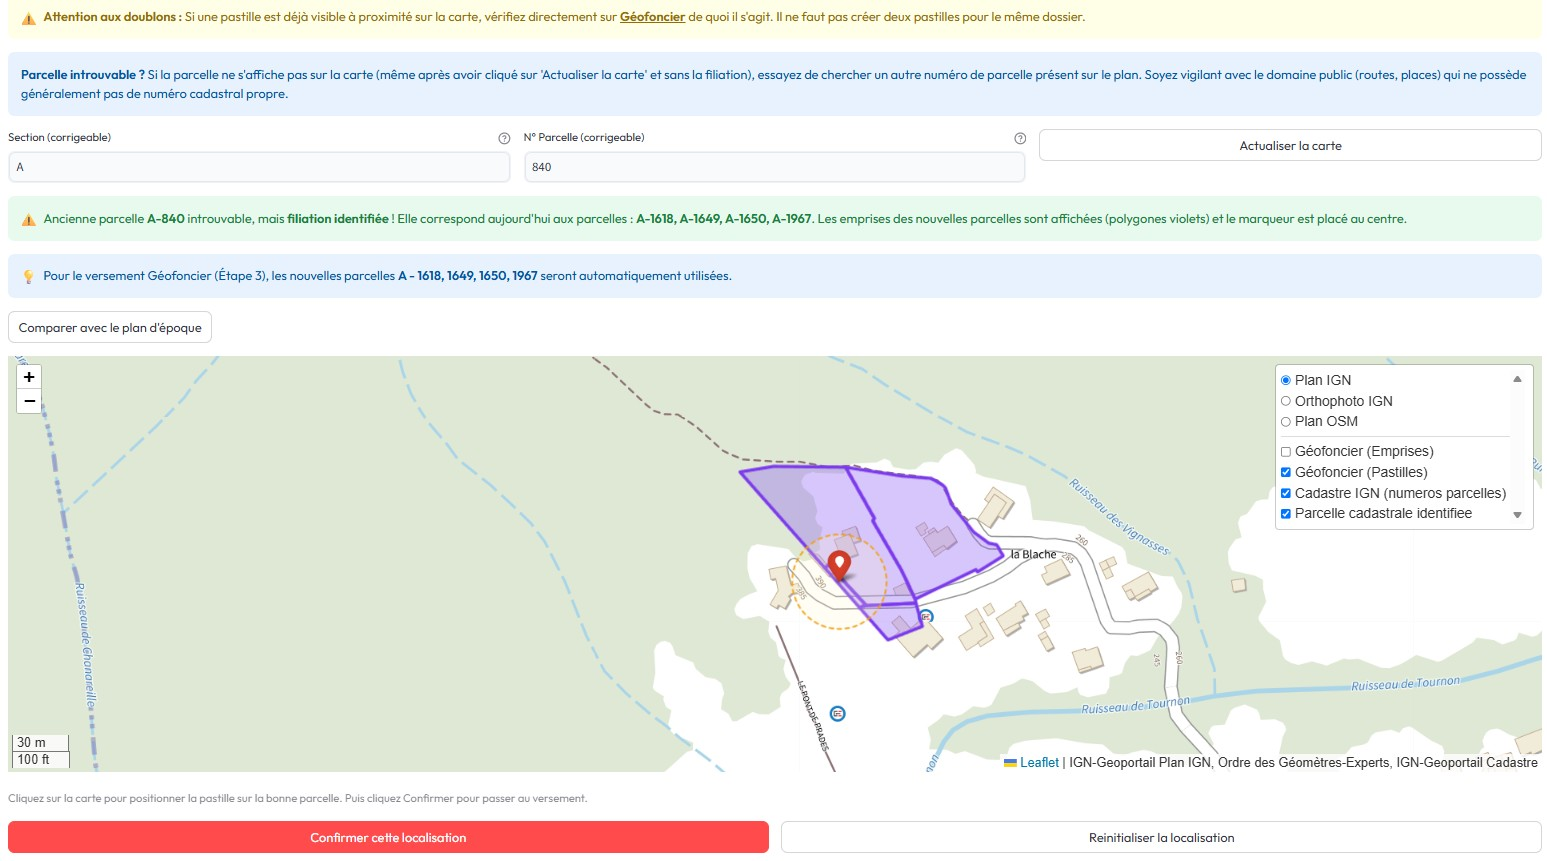
\includegraphics[width=0.95\textwidth]{img/Etape_2_localisation_cartographie.jpg}
  \caption{Étape 2 -- Carte interactive avec fond cadastral IGN, gestion des filiations de parcelles et contrôle des doublons Géofoncier.}
  \label{fig:etape2_carte}
\end{figure}

Après cette validation, l'application oriente l'utilisateur vers la phase finale du traitement.


\subsection{Exportation et versement sur Géofoncier}

La dernière étape regroupe l'ensemble des informations collectées pour l'envoi vers Géofoncier. Le récapitulatif est divisé en deux sections : la première rassemble les données du cabinet (cabinet créateur, détenteur, géomètre et référence interne du dossier), tandis que la seconde récapitule les éléments cadastraux (code INSEE, commune, section, parcelles retenues et nature de l'acte). Le type d'opération est rempli automatiquement. L'opérateur précise la date, choisit le statut dans la liste déroulante et vérifie les éventuels messages d'avertissement. Enfin, l'activation du bouton \enquote{Créer le dossier sur Géofoncier} déclenche l'envoi vers l'API REST pour inscrire le dossier sur la plateforme.

\begin{figure}[H]
  \centering
  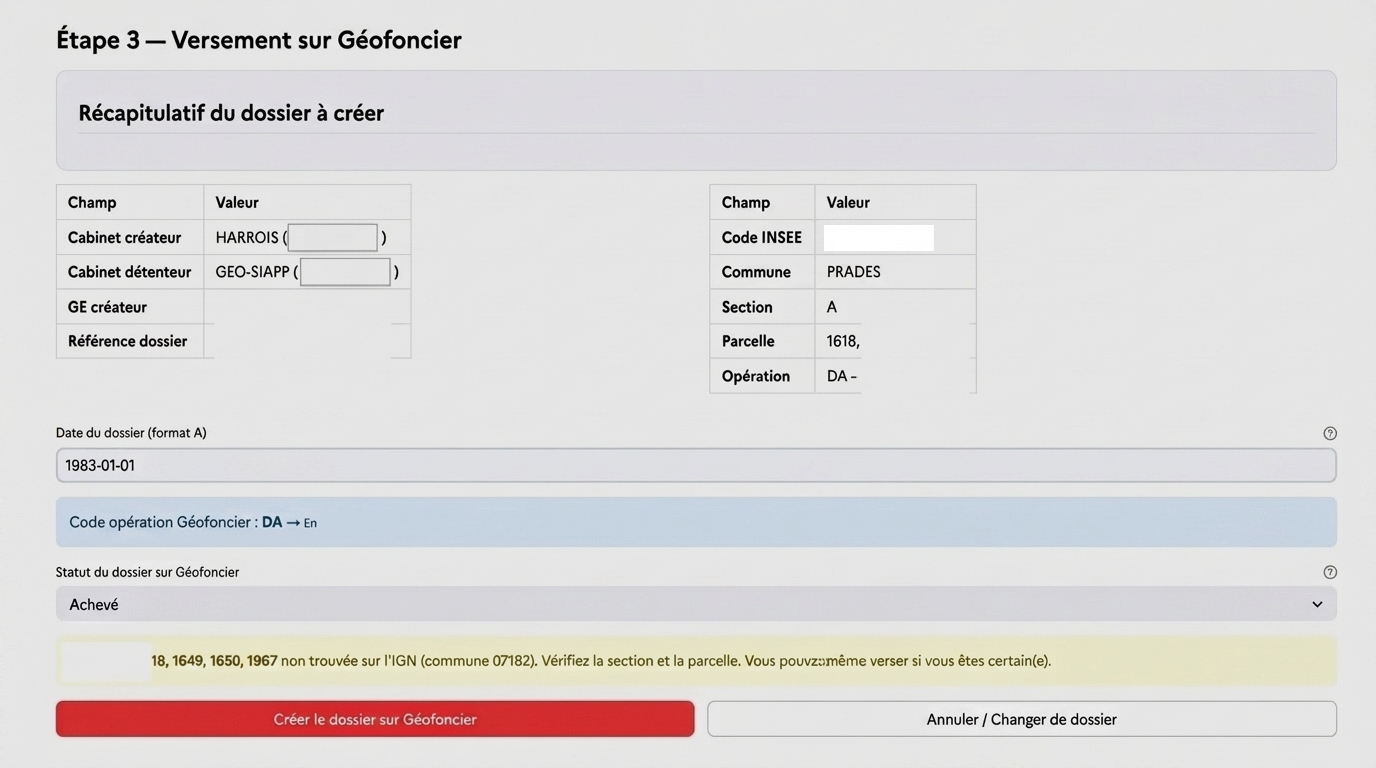
\includegraphics[width=0.90\textwidth]{img/Etape3_Versement_geofoncier.jpg}
  \caption{Étape 3 -- Formulaire de versement sur Géofoncier avec récapitulatif des données du cabinet et des éléments cadastraux.}
  \label{fig:etape3_versement}
\end{figure}



\subsection{Numérisation des répertoires anciens}

La recherche dans les répertoires présentée à la section précédente repose sur des fichiers Excel qui listent l'ensemble des dossiers archivés par chaque géomètre. Ces fichiers n'existaient pas sous forme numérique pour certains, les répertoires du Géomètre A et du Géomètre B n'étaient disponibles que sous forme de registres papier manuscrits, numérisés en PDF. Deux programmes d'extraction indépendants ont été développés dans le cadre de ce PFE pour produire ces bases de données, chacun adapté à la mise en page et à la nature des écritures du géomètre concerné. Les deux suivent la même structure en deux temps : une phase d'extraction automatique, suivie d'une interface de validation. Chacun est lancé par un fichier \texttt{.bat} qui installe les dépendances manquantes, exécute l'extraction, puis ouvre l'interface dans le navigateur web.

Le registre du Géomètre A (Figure~\ref{fig:geom_a_liste}) se présente sous la forme d'un tableau à double colonne : la colonne de gauche liste les anciens propriétaires, la colonne de droite les nouveaux. Les années sont imprimées en rouge et encadrent les blocs de dossiers. Les numéros de dossiers, portés dans la marge gauche, servent d'ancres pour délimiter chaque entrée. Le script \texttt{extract\_geometre\_A.py} traite les PDF page par page à haute résolution (environ 288 DPI). EasyOCR retourne les blocs de texte avec leurs coordonnées. Une analyse de l'image localise ensuite la ligne verticale qui sépare les deux colonnes de propriétaires. Les blocs dont le fond est détecté comme rouge en espace HSV sont extraits comme marqueurs d'année. Une correction rectifie les confusions dues au soulignement rouge qui coupe certains chiffres (un \texttt{1913} lu par l'OCR peut être corrigé en \texttt{1973} si l'année sort de la plage attendue). Les numéros de dossiers dans la marge gauche servent d'ancres : chaque bloc de texte est assigné au dossier dont l'ancre est la plus proche en Y, puis affecté à la colonne \textit{Anciens} ou \textit{Nouveaux} selon sa position par rapport au séparateur. Les communes sont résolues par correspondance (\texttt{rapidfuzz}) contre la liste des communes de l'Ardèche et de la Drôme. Les dossiers extraits sont enregistrés dans un fichier JSON intermédiaire en attendant la validation.

\begin{figure}[H]
  \centering
  \setlength{\fboxsep}{0pt}%
  \setlength{\fboxrule}{0.6pt}%
  \fbox{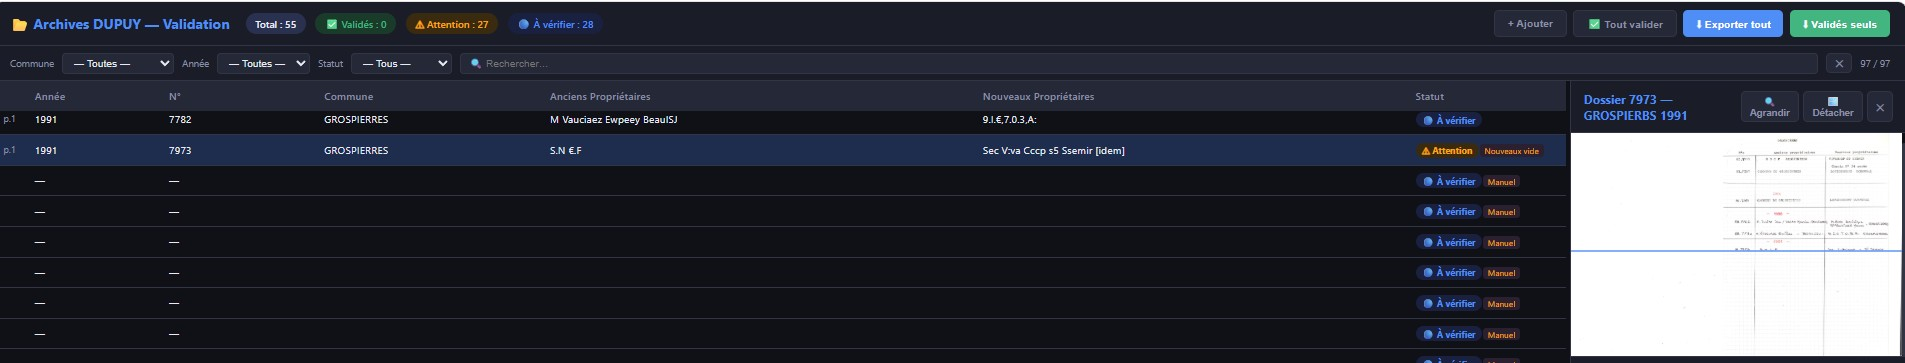
\includegraphics[width=0.95\linewidth]{img/5.5_reprtoire_A_liste.jpg}}
  \caption{Interface de validation du répertoire du Géomètre A (port 5050) -- Vue synthétique et liste des dossiers extraits.}
  \label{fig:geom_a_liste}
\end{figure}

\clearpage

\begin{wrapfigure}{r}{0.46\textwidth}
  \vspace{-1.2em}
  \centering
  \setlength{\fboxsep}{0pt}%
  \setlength{\fboxrule}{0.6pt}%
  \fbox{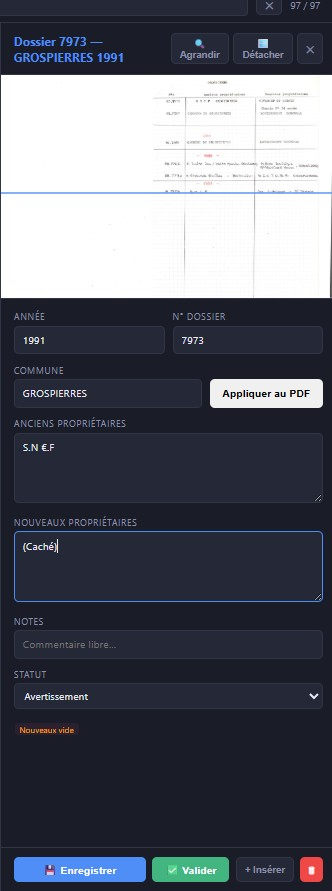
\includegraphics[width=\linewidth]{img/5.5_reprtoire_A_infos.jpg}}
  \caption{Interface du Géomètre A (port 5050) -- Fiche détaillée et édition des champs.}
  \label{fig:geom_a_infos}
  \vspace{-1em}
\end{wrapfigure}

L'interface de validation est un serveur local accessible sur \texttt{http://localhost:5050}. Elle s'articule autour de deux vues principales. La première vue (Figure~\ref{fig:geom_a_liste}) présente la liste des dossiers extraits sous la forme d'un tableau synthétique, permettant à l'opérateur de parcourir rapidement l'ensemble des affaires répertoriées.

Lorsqu'un dossier est sélectionné dans le tableau, l'interface affiche la fiche détaillée (Figure~\ref{fig:geom_a_infos}) regroupant l'ensemble des champs d'indexation (commune, année, référence du dossier, anciens et nouveaux propriétaires). L'opérateur peut y consulter le scan de la page originale, réexécuter l'OCR sur une zone spécifique ou corriger directement les valeurs extraites.

À la validation, les corrections sont fusionnées dans le fichier Excel maître (\texttt{Repertoire\_}\linebreak[0]\texttt{Archives\_}\linebreak[0]\texttt{geometre\_A.xlsx}), en utilisant les clés d'indexation (Commune, Année, N° Dossier) pour éviter tout doublon. Ce fichier est également synchronisé sur le serveur partagé du cabinet. (Les captures grand format sont consultables en Annexe G).

Le traitement du registre du Géomètre A repose sur une logique de découpage par colonnes fixes. Les lignes de séparation imprimées en rouge permettent d'isoler les noms des anciens et des nouveaux propriétaires avec un bon taux de réussite. En cas de doute sur une lettre ou un nom propre, l'interface de validation permet à l'opérateur de visualiser immédiatement le bloc d'image découpé et de rectifier la saisie en quelques secondes.

Le registre du Géomètre B présente des difficultés plus importantes en raison de son écriture manuscrite variée et de l'absence de colonnes imprimées. Pour limiter les erreurs de lecture, le script d'extraction applique un prétraitement d'image adaptatif qui redresse la page, ajuste le contraste et cherche les vallées de texte avant de transmettre l'image au modèle VLM. Malgré ces préconisations, les zones raturées et les écritures cursives inclinées exigent une relecture attentive par l'utilisateur avant l'enregistrement final dans le registre maître.

Le registre du Géomètre B est d'une nature différente : il s'agit d'un livret à double page (un aperçu de ce type de registre est présenté en Figure~\ref{fig:registre_ancien}), où chaque ligne correspond à un dossier, répartie en cinq colonnes (numéro de dossier, date, commune, désignation de l'affaire, donneur d'ordre). L'écriture est manuelle et les colonnes ne sont pas toujours parfaitement alignées, ce qui rend l'OCR seul insuffisant. Le script \texttt{extract\_geometre\_B.py} adopte pour cela une stratégie hybride. Les PDF sont rendus à haute résolution et les doubles pages découpées au milieu. Un redressement automatique corrige les légers défauts d'angle liés à la numérisation du livret. EasyOCR localise ensuite les boîtes de texte et les regroupe par ligne selon leur proximité verticale, et les en-têtes de colonnes sont exclus automatiquement. Chaque ligne est découpée en image, sur laquelle des repères verticaux sont tracés à des positions connues car régulières pour matérialiser les séparations entre colonnes. Cette image annotée est envoyée au modèle IA MiniCPM-V (exécuté localement via Ollama) avec un prompt qui lui demande de lire chaque colonne et de retourner un JSON avec les clés \texttt{N\_Dossier}, \texttt{Date}, \texttt{Commune}, \texttt{Affaire} et \texttt{Client}. Les réponses sont ensuite nettoyées et validées : format de date, résolution de la commune par correspondance contre les communes de l'Ardèche. Un filtre anti-hallucination vide la case commune si aucune correspondance locale n'est trouvée.

L'interface de validation est la même que celle du Géomètre A, accessible sur le port local \texttt{5051}. Elle s'adapte aux informations propres au registre du Géomètre B (numéro de dossier, date, commune, désignation de l'affaire et client). À la validation, les données corrigées sont enregistrées dans un fichier Excel maître distinct (\texttt{Repertoire\_Archives\_}\linebreak[0]\texttt{geometre\_B.xlsx}), en utilisant le triplet (N° Dossier, Date, Commune) comme clé primaire, et le fichier est synchronisé sur le réseau du cabinet.

Cette étape de numérisation préalable des registres permet de construire la base d'indexation indispensable à la recherche d'antériorités. Comme mentionné lors de l'étude des limites au chapitre~\ref{sec:limites_perspectives}, la qualité d'extraction sur ces registres varie selon la régularité des tracés et la présence de lignes de séparation imprimées.


\subsection{Résolution et correction des noms de communes}
\label{subsec:appariement_communes}

Lors de l'extraction des données par les modèles de lecture, le texte transcrit pour les noms de communes contient souvent des erreurs de nature variée : un caractère mal lu, une majuscule différente, une abréviation ou une ligature ancienne. Par exemple, le moteur peut lire \texttt{St-Pierreville} au lieu de \texttt{Saint-Pierreville}, ou \texttt{Chomerac} au lieu de \texttt{Chomérac}. Ces erreurs empêchent une correspondance parfaite avec la liste de référence des communes, ou à l'inverse peuvent faire correspondre une détection à la mauvaise commune.

Pour corriger automatiquement ces écarts, le script s'appuie sur une recherche par correspondance approximative entre la chaîne lue et les noms de communes issus du code officiel de l'INSEE~\citep{insee_cog}. La mesure de similarité utilisée est la \textit{distance de Levenshtein}, qui compte le nombre minimal d'opérations élémentaires (insertion, suppression ou substitution d'un caractère) nécessaires pour transformer une chaîne en une autre~\citep{levenshtein_binary_1966}.

\begin{equation}
  d(a, b) = \min
  \begin{cases}
    d(a_{1..n-1},\, b) + 1 & \text{(suppression)} \\
    d(a,\, b_{1..m-1}) + 1 & \text{(insertion)} \\
    d(a_{1..n-1},\, b_{1..m-1}) + \mathbf{1}_{[a_n \neq b_m]} & \text{(substitution)}
  \end{cases}
\end{equation}

où $a$ est la chaîne extraite, $b$ le nom de commune de référence, $n = |a|$ et $m = |b|$.Le score exprimé sur 100 par la bibliothèque \texttt{rapidfuzz} correspond à un ratio de similarité dérivé de cette distance : $\text{ratio}(a, b) = 100 \times \left(1 - \frac{d(a,b)}{\max(|a|,|b|)}\right)$. Ce score est calculé en quelques microsecondes grâce aux optimisations SIMD de RapidFuzz, ce qui rend la recherche instantanée même sur la liste complète des 40000 communes françaises.

Le script applique plusieurs variantes de correspondance en parallèle pour traiter les cas les plus fréquents :

\begin{itemize}
  \item Correspondance directe normalisée : les deux chaînes sont mises en minuscules, les accents supprimés et les tirets remplacés par des espaces avant la comparaison. Cela résout les différences de casse ou de ponctuation sans pénaliser la distance.
  \item Correspondance sur les mots : les mots de chaque chaîne sont triés alphabétiquement avant la comparaison. Ce traitement gère les inversions d'ordre, comme \texttt{Bourg-Saint-Andéol} comparé à \texttt{Saint-Andéol-de-Berg}.
  \item Correspondance partielle : un sous-segment de la chaîne est comparé au nom de référence. Cela couvre les cas d'abréviation, comme \texttt{St-Didier} pour \texttt{Saint-Didier-sous-Aubenas}.
\end{itemize}

Le score retenu est le maximum des trois variantes. Si ce score est supérieur ou égal à un seuil paramétrable, la correspondance est acceptée et le nom et le code INSEE associés sont affichés dans l'interface. Si le score est inférieur au seuil, le champ est marqué comme incertain et un avertissement invite l'opérateur à corriger manuellement la valeur, conformément aux règles de contrôle définies au chapitre~\ref{sec:architecture}.

\begin{figure}[H]
  \centering
  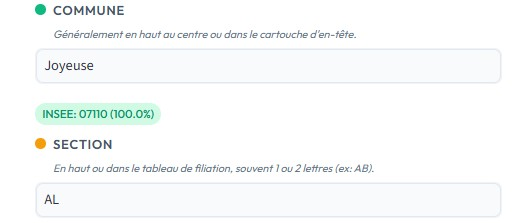
\includegraphics[width=0.65\textwidth]{img/zoom_commune.jpg}
  \caption[Résultat de l'appariement pour le champ Commune]{Résultat de l'appariement : le champ Commune affiche la valeur normalisée \texttt{Joyeuse} avec son code INSEE et un score de confiance de 100\,\%.}
  \label{fig:appariement_commune}
\end{figure}

Ce système automatise la plupart des corrections. Sur les lots testés, plus de 95\,\% des noms de communes erronés sont résolus sans intervention humaine, y compris les cas d'accents manquants, de préfixes abrégés (Saint/St, Sainte/Ste) et de séparateurs variables (tiret, espace, trait d'union).

Dans les départements ruraux et même ailleurs, plusieurs fusions de communes sont intervenues au cours des cinquante dernières années. Par exemple, les anciennes communes de Vallon-Pont-d'Arc et de Lagorce ou les anciennes sections d'Aubenas ont vu leurs dénominations évoluer. Ainsi, lorsqu'un acte ancien mentionne une commune aujourd'hui déléguée ou rattachée, la base de correspondance conserve les anciens codes INSEE associés à leur commune actuelle de rattachement. Le script propose alors à l'opérateur le nom actuel tout en gardant l'ancien nom en note d'archive, afin de garantir la validité du versement sur le portail Géofoncier tout en préservant la valeur du document.

Pour accélérer le calcul lors du traitement de gros volumes de documents, la recherche par correspondance s'appuie sur un index pré-calculé chargé en mémoire au démarrage de l'application. Cet index regroupe les noms de communes par département et par préfixe alphabétique, ce qui réduit le nombre de comparaisons nécessaires et permet d'obtenir une réponse en moins d'une milliseconde par mot.

Pour chaque proposition de correction générée par la comparaison de Levenshtein, l'interface conserve le détail de la chaîne initiale extraite par l'OCR, la méthode de calcul ayant obtenu le meilleur score (directe, par tokens ou partielle), ainsi que les deux communes candidates arrivées en deuxième et troisième positions. Ces informations permettent à l'opérateur de comprendre rapidement l'origine d'une alerte lors d'un doute sur une commune limitrophe.

\subsection{Bilan de la phase de fiabilisation}

La combinaison du nettoyage (correction des erreurs de saisie, résolution des communes, filiation cadastrale) et du contrôle humain via les interfaces web permet d'obtenir des données fiables et directement exploitables. Les incertitudes d'extraction sont rapidement corrigées par l'opérateur, ce qui garantit la qualité finale des bases de données.

Enfin, cette étape de fiabilisation prépare les données pour la dernière phase du projet. Les répertoires propres et les dossiers correctement géolocalisés peuvent à présent être transmis de manière automatique au portail national Géofoncier, sujet présenté dans le chapitre suivant (chapitre~\ref{sec:integration}).






\clearpage
% !TeX root = main.tex

\section{Intégration à Géofoncier et évaluation des résultats}
\label{sec:integration}

Ce chapitre présente la dernière phase du traitement : le versement sur Géofoncier. Il décrit d'abord en détail comment l'appel à l'API est géré techniquement, puis expose le mode de traitement, avant de suivre un dossier réel de bout en bout et de conclure sur une évaluation du système.

\subsection{Fonctionnement du versement}

Le chapitre~\ref{sec:analyse_metier} a présenté la structure de l'API REST Géofoncier et le format des données qu'elle attend. Cette section décrit comment le script \texttt{geofoncier\_api.py} met en pratique ces échanges, du jeton d'authentification jusqu'à l'upload du document source.

Les identifiants du cabinet (login et mot de passe Géofoncier) sont stockés dans un fichier \texttt{.env} local, qui n'est jamais partagé ni versionné. L'authentification repose sur une requête \texttt{GET /token} avec une en-tête \texttt{Authorization: Basic base64(login:password)}.

Au démarrage de l'application, la fonction \texttt{get\_valid\_token()} décode la date d'expiration inscrite dans le jeton JWT (champ \texttt{exp}) et calcule le temps restant. Si l'expiration est à moins de 30 minutes, un nouveau jeton est demandé automatiquement. Ce mécanisme est entièrement transparent pour l'opérateur. La durée de validité réelle d'un jeton est de 10 heures.

En cas d'échec du renouvellement, l'ancienne valeur du jeton est conservée en mémoire et l'interface affiche un avertissement. Si aucun jeton valide n'est disponible au moment du versement, l'API retourne un \texttt{401 Unauthorized}, que l'interface traduit en message explicite.

Lorsque l'opérateur clique sur \enquote{Créer le dossier sur Géofoncier}, l'application construit le dictionnaire de données à partir de toutes les informations collectées lors des étapes précédentes. La fonction \texttt{create\_geofoncier\_dossier()} assemble ensuite le payload JSON avant l'envoi. Ce dictionnaire rassemble les identifiants Géofoncier du cabinet créateur (\texttt{enr\_cab\_createur}, par exemple \texttt{1987I004169}) et du cabinet détenteur (\texttt{enr\_cab\_detenteur}), la référence interne du dossier (\texttt{enr\_ref\_dossier}, limitée à 15 caractères), le code INSEE à 5 chiffres (\texttt{enr\_code\_insee}), ainsi que la date de l'opération au format ISO 8601 (\texttt{enr\_date\_dossier}). Il spécifie aussi le code d'opération (\texttt{op\_code}, comme \texttt{Em} pour une modification parcellaire ou \texttt{Eb} pour un bornage), la liste des parcelles cadastrales, les coordonnées Lambert-93 du marqueur sur la carte (\texttt{localisant}), le numéro DMPC formaté (\texttt{dmpc\_ref}) et le statut du dossier (\texttt{enr\_statut}).

Détail des éléments transmis dans ce dictionnaire :
\begin{itemize}
  \item Identifiants du cabinet : les champs \texttt{enr\_cab\_createur} et \texttt{enr\_cab\_detenteur} reçoivent le numéro d'inscription du cabinet à l'Ordre des Géomètres-Experts.
  \item Référence et commune : le champ \texttt{enr\_ref\_dossier} enregistre la référence interne (15 caractères maximum), \texttt{enr\_code\_insee} le code de la commune à 5 chiffres, et \texttt{enr\_date\_dossier} la date au format ISO.
  \item Type d'opération : le champ \texttt{op\_code} précise la nature de l'acte (\texttt{Em} pour division, \texttt{Eb} pour bornage), et \texttt{enr\_statut} indique le niveau de validation.
  \item Localisant géométrique : l'objet \texttt{localisant} contient une structure de point GeoJSON avec les coordonnées du marqueur calculées en Lambert-93 (EPSG:2154).
  \item Parcelles concernées : la liste \texttt{parcelles} rassemble les objets précisant la section cadastrale et le numéro de chaque parcelle modifiée.
\end{itemize}

Chaque champ fait l'objet d'un contrôle automatique avant la requête, comme expliqué lors de la fiabilisation au chapitre~\ref{sec:fiabilisation}. Si le code INSEE ou les coordonnées sont absents, le script bloque la préparation et alerte l'opérateur dans l'interface.

Avant l'envoi, le dictionnaire est converti en JSON. Les coordonnées spatiales en Lambert-93 sont arrondies à deux décimales (précision centimétrique). Les chaînes de caractères sont encodées en UTF-8 pour prévenir toute altération des caractères accentués lors du transit HTTP.

Le transfert des requêtes vers le serveur de Géofoncier s'appuie sur la bibliothèque \texttt{requests} avec une gestion des délais d'attente. Si le serveur de la plateforme met plus de 15 secondes à répondre (en période de forte charge), l'application effectue jusqu'à trois tentatives successives avec un délai d'attente avant de lever une exception et de proposer une sauvegarde locale temporaire à l'utilisateur.

Le marqueur positionné par l'opérateur sur la carte est en coordonnées géographiques WGS84 (latitude/longitude). L'API Géofoncier attend des coordonnées en Lambert-93 (système officiel français, EPSG:2154). La conversion est assurée par la fonction \texttt{latlon\_to\_lambert93()}, qui utilise la bibliothèque \texttt{pyproj} si elle est disponible, ou à défaut une formule intégrée.

La requête \texttt{POST /dossiersoge/dossiers/} est envoyée avec le payload JSON dans le corps et le jeton dans l'en-tête \texttt{Authorization}. L'appel est synchrone : l'interface affiche un spinner pendant l'envoi.

En cas de succès, l'API retourne un code \texttt{201 Created} et un objet JSON contenant le champ \texttt{id} du dossier créé. Ce champ est affiché directement dans l'interface et enregistré dans le CSV de travail.

L'API peut également rejeter le champ \texttt{dmpc\_ref} si le format du numéro de DA ne correspond pas à celui attendu côté serveur. Le script gère ce cas avec un mécanisme de repli : il détecte le code d'erreur \texttt{400} associé à ce champ, supprime \texttt{dmpc\_ref} du payload et relance la requête sans lui. Le dossier est ainsi créé même si la référence DMPC n'a pas pu être attachée.

Après la création réussie du dossier, une deuxième requête \texttt{POST /dossiersoge/documents/} est envoyée en \texttt{multipart/form-data} pour attacher le fichier PDF au dossier. Le type MIME est détecté automatiquement depuis l'extension du fichier (\texttt{.pdf}, \texttt{.tif}, \texttt{.jpg}, etc.). Si le fichier source est introuvable dans le dossier d'entrée, l'interface signale l'absence sans bloquer : le dossier est déjà créé sur Géofoncier.

Plusieurs situations peuvent provoquer un échec lors du versement. Le Tableau~\ref{tab:erreurs_api} liste les principaux cas identifiés et les réponses apportées par le système.


\begin{table}[H]
  \centering
  \caption{Principaux cas d'erreur lors du versement sur l'API Géofoncier.}
  \label{tab:erreurs_api}
  \small
  \begin{tabular}{p{3.5cm}p{3.5cm}p{5cm}}
    \toprule
    \textbf{Cause} & \textbf{Code HTTP} & \textbf{Réponse du système} \\
    \midrule
    Token expiré ou invalide & \texttt{401 Unauthorized} & Message d'erreur dans l'interface, invitation à relancer l'application. \\
    \addlinespace
    Code INSEE manquant ou invalide & \texttt{400 Bad Request} & Blocage du bouton de versement dès la saisie ; le champ est marqué en rouge. \\
    \addlinespace
    Champ \texttt{dmpc\_ref} refusé & \texttt{400 Bad Request} & Repli automatique : nouvelle tentative sans ce champ. \\
    \addlinespace
    Données manquantes (référence vide) & Bloqué côté client & Le bouton est désactivé tant que la référence dossier n'est pas renseignée. \\
    \addlinespace
    Perte réseau pendant l'envoi & Exception Python & Message d'erreur avec le détail du payload envoyé pour diagnostic. \\
    \bottomrule
  \end{tabular}
\end{table}

Dans tous les cas d'échec, l'interface affiche le message d'erreur retourné par l'API et propose un panneau dépliable avec le contenu exact du payload, pour permettre de diagnostiquer la cause sans avoir à consulter les logs.

\subsection{Sécurisation du versement et traçabilité des échanges}

La transmission de données foncières vers une plateforme nationale exige un niveau élevé de contrôle afin de prémunir le cabinet contre tout risque de publication erronée ou de mauvaise interprétation.

\textbf{Contrôle de doublons et vérification d'intégrité avant envoi.} Avant de déclencher l'appel REST vers l'API Géofoncier, l'application interroge le registre local de suivi pour vérifier si la référence du dossier ou le document source a déjà fait l'objet d'une publication réussie. Si un doublon potentiel est détecté, l'interface affiche un message de mise en garde et bloque l'envoi direct, demandant une confirmation explicite à l'opérateur. De plus, une empreinte numérique (hash SHA-256) du fichier PDF source est calculée au moment du chargement. Cette empreinte est conservée dans l'historique local pour garantir qu'aucune modification ultérieure du fichier n'intervienne sans que la traçabilité ne soit rompue.

\textbf{Protocoles de communication des identifiants.} Toutes les requêtes transmises à l'API Géofoncier s'effectuent exclusivement en HTTPS via TLS 1.3, ce qui garantit le chiffrement de bout en bout des échanges sur le réseau. Les jetons JWT d'authentification sont stockés temporairement en mémoire vive au cours de la session applicative et ne sont jamais enregistrés dans des fichiers de sous-produits ou de journaux d'événements. Cette séparation stricte protège les identifiants professionnels du cabinet contre toute extraction non autorisée.

\textbf{responsabilité déontologique.} En vertu des règles déontologiques régissant la profession de géomètre-expert, toute publication sur le portail Géofoncier engage la responsabilité du cabinet détenteur du fonds. Pour répondre à cette exigence, chaque action de versement donne lieu à la rédaction automatique d'un journal d'audit infalsifiable. Ce journal consigne l'identifiant de l'opérateur connecté, l'adresse IP de la station de travail, l'horodatage exact au format UTC, la référence du dossier, le code INSEE de la commune ainsi que le contenu intégral de la réponse HTTP renvoyée par le serveur distant. Ces données fournissent une preuve technique incontestable en cas de contrôle de conformité ou de recherche d'historique.

\subsection{Mode de traitement par lot : \texttt{export\_geofoncier.py}}

En complément de l'interface de validation, un script de service (\texttt{export\_geofoncier.py}) permet de traiter des lots de documents sans intervention manuelle document par document. Ce script est prévu pour être lancé en tâche de fond, en parallèle du traitement OCR.

Son fonctionnement repose sur une boucle infinie qui scanne le dossier \texttt{outputs/} toutes les 30 secondes. À chaque itération, le script liste tous les fichiers JSON produits par la chaîne d'extraction (nommés selon le schéma \texttt{*\_plan\_*.json}) qui n'ont pas encore été traités. Pour chacun, il appelle \texttt{create\_geofoncier\_dossier()} avec le JSON comme source de données, puis tente d'uploader le PDF associé depuis \texttt{inputs/}. Une fois le traitement terminé (avec succès ou échec définitif), le fichier JSON est déplacé dans le sous-dossier \texttt{outputs/archives\_publiees/} pour ne pas être retraité au prochain scan.

Ce mode est particulièrement adapté au traitement de fonds entiers : une boîte de documents scannés peut être injectée dans \texttt{inputs/}, l'extraction automatique tourne la nuit, et les dossiers sont versés sur Géofoncier au fur et à mesure que les JSON sont produits. La supervision humaine reste indirecte : l'opérateur consulte le registre de suivi le lendemain pour vérifier les résultats.

\textbf{Le registre de suivi.} Après chaque versement, le script enregistre une entrée dans deux fichiers stockés dans le dossier \texttt{suivi\_geofoncier/}. Le premier fichier, \texttt{suivi\_publications.json}, conserve l'historique complet des versements (horodatage, commune, code INSEE, géomètre, référence du dossier, identifiant Géofoncier, nom du document source et statut final). Le second, \texttt{suivi\_publications.csv}, propose un tableau équivalent trié par commune puis par date, directement exploitable sous Excel ou LibreOffice.

Ces fichiers constituent la trace locale du travail effectué. Ils permettent aux associés du cabinet de savoir exactement quels dossiers ont été versés, à quelle date et sous quel identifiant Géofoncier, sans avoir à interroger l'API ni à consulter le portail.

En cas de coupure de réseau ou de panne temporaire du serveur distant pendant l'exécution par lot, le script conserve les requêtes non abouties dans une file d'attente locale de réessai. Les fichiers JSON correspondants ne sont pas déplacés vers le sous-dossier d'archivage, mais restent en attente. Dès la reconnexion au réseau, le script reprend l'envoi de la file d'attente à partir du dernier point d'échec sans risquer de créer des doublons d'actes sur le serveur Géofoncier.


\subsection{Déroulement d'un cas d'étude : commune de Prades}

Cette section suit le traitement d'un dossier réel de bout en bout, depuis le document papier jusqu'à la pastille créée sur Géofoncier.

Le document traité est un DMPC numérisé, issu du fonds du cabinet, concernant la commune de Prades (code INSEE~: \texttt{07182}), section cadastrale A. Il s'agit d'un formulaire imprimé d'une page, complété à la main. Le fichier est fourni au programme sous forme de PDF, placé dans le dossier d'entrée.

Le script de classification analyse le fichier et le reconnaît comme un DMPC en quelques secondes, sur la base de sa structure. Le modèle VLM traite ensuite les onze zones d'intérêt découpées par YOLOv8 sur la page. L'extraction automatique identifie la commune de Prades avec un indice de confiance de 92\,\% (validé à 100\,\% dans le référentiel de l'Ardèche), la section cadastrale A à 95\,\%, ainsi que le numéro d'ordre 3854 à 70\,\% (la présence d'un chiffre parasite 4 étant provoquée par le coin d'un tampon en marge, rapidement relevé par le contrôle de cohérence). Le nom du géomètre est détecté par balayage textuel (80\,\%), et la nature de l'acte est déduite comme étant un bornage.

Le contrôle de cohérence en quatre couches retourne un statut conforme avec un score de 100\,\%. L'image annotée générée par le traitement est reproduite en Figure~\ref{fig:harrois_annote}.

\begin{figure}[H]
  \centering
  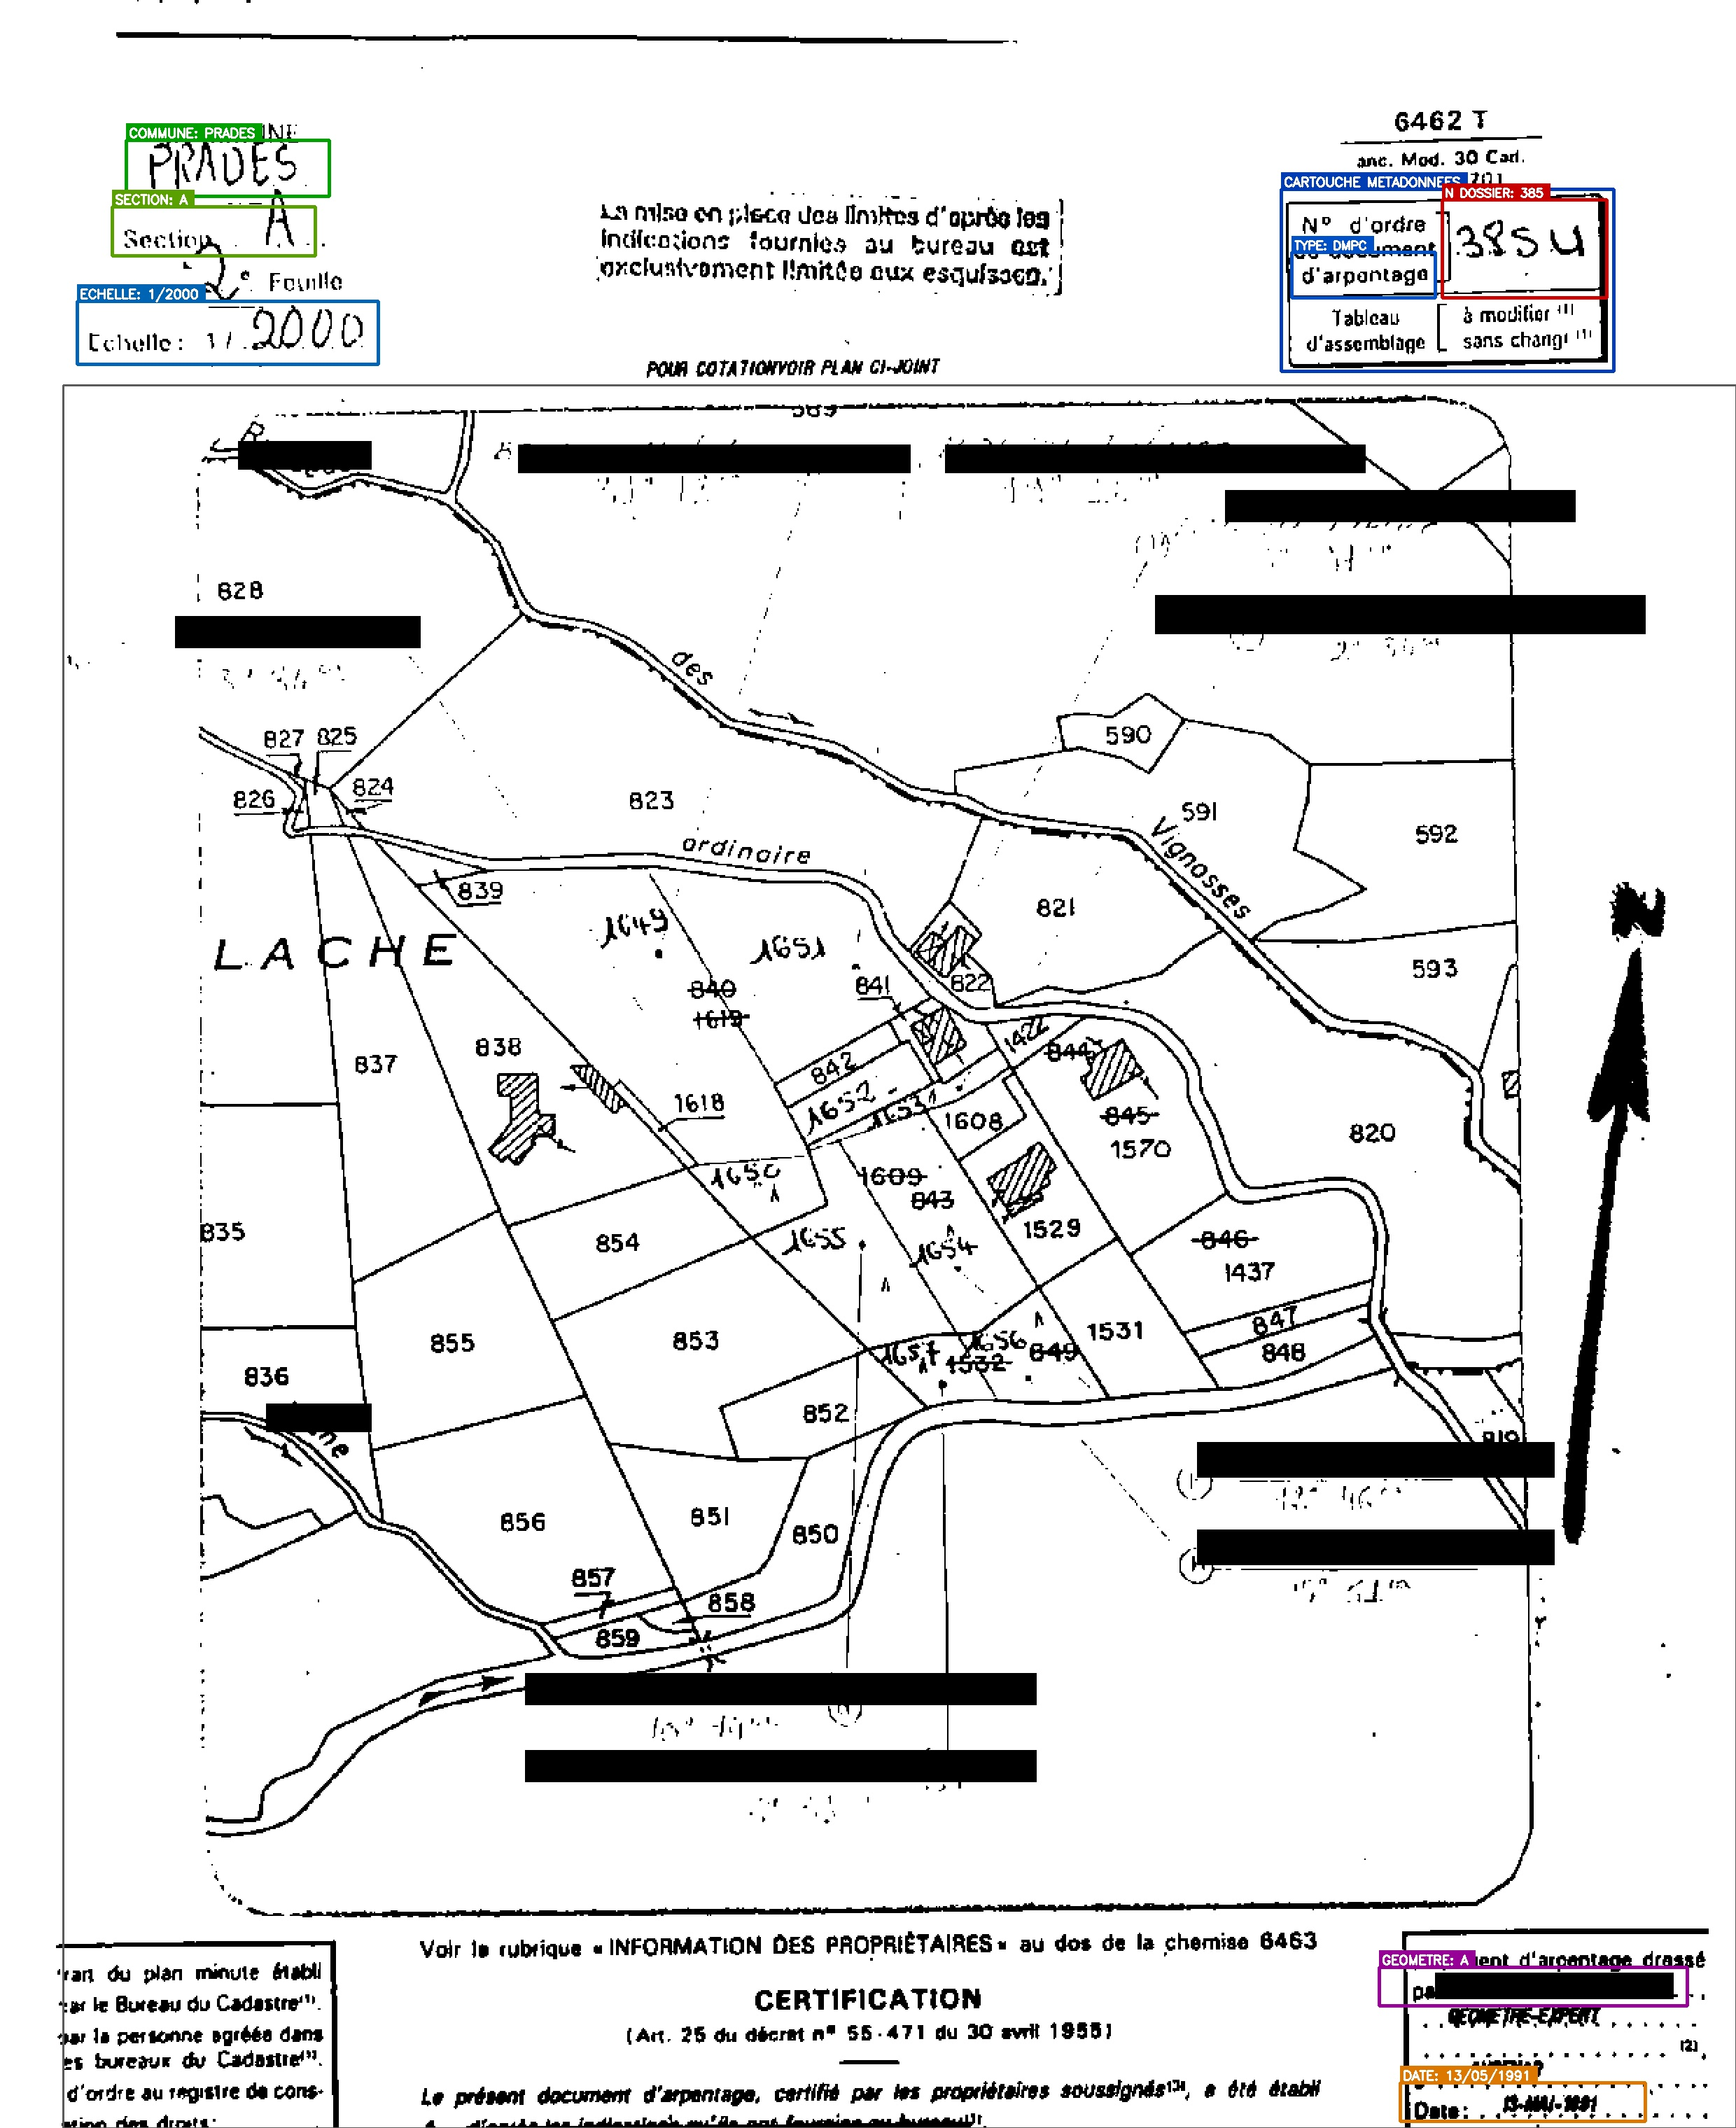
\includegraphics[width=0.85\textwidth]{img/harrois_annote.jpg}
  \caption{Image annotée du DMPC de Prades : les zones d'intérêt détectées par YOLOv8 sont encadrées sur le document source.}
  \label{fig:harrois_annote}
\end{figure}

L'interface de validation (présentée au chapitre~\ref{sec:fiabilisation}) affiche directement les données extraites du document. L'opérateur contrôle les informations, comme la commune ou la section, et corrige les petites erreurs si nécessaire, par exemple le numéro d'ordre (\texttt{3854} $\rightarrow$ \texttt{385}) perturbé par un tampon en marge.

À l'étape 1, la recherche dans le répertoire numérisé retrouve la référence interne du dossier au cabinet.

À l'étape 2, la carte interactive affiche la parcelle sur le fond cadastral IGN. L'opérateur vérifie qu'aucune pastille n'existe déjà à cet endroit, puis confirme la localisation. Les coordonnées GPS sont automatiquement converties en Lambert-93 par la fonction \texttt{latlon\_to\_lambert93()}.

À l'étape 3, l'interface affiche le récapitulatif complet des données avant l'envoi.

L'opérateur clique sur \enquote{Créer le dossier sur Géofoncier}. L'API retourne un code \texttt{201 Created} avec l'identifiant du dossier créé. Le fichier PDF est automatiquement joint au dossier dans la foulée. La confirmation s'affiche dans l'interface (Figure~\ref{fig:confirmation_geofoncier}).

\begin{figure}[H]
  \centering
  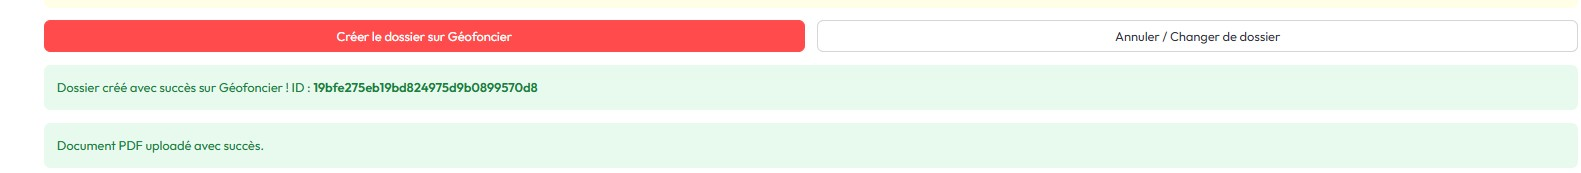
\includegraphics[width=0.95\textwidth]{img/6_succes_pastille.jpg}
  \caption{Confirmation de la création du dossier sur Géofoncier.}
  \label{fig:confirmation_geofoncier}
\end{figure}

Le dossier est désormais visible sur GéofoncierEXPERT sous forme de pastille géolocalisée, consultable par l'ensemble de la profession. Le statut de la ligne dans le fichier CSV local est automatiquement mis à jour avec la mention \texttt{Versé sur Géofoncier} et l'horodatage exact de la publication.

\subsection{Évaluation des performances}

Sans l'outil, retrouver un dossier dans les archives physiques prend au minimum une dizaine de minutes lorsque les boîtes sont bien organisées. Ce temps s'allonge si les dossiers sont mal rangés, si le registre du géomètre correspondant n'est pas encore numérisé, ou si plusieurs affaires correspondent aux mêmes références cadastrales.

Avec cet outil, le déroulement ne demande que quelques minutes de traitement OCR automatique (environ dix minutes pour un lot complet de cinq à six documents), suivies de deux ou trois minutes de contrôle dans l'interface pour relire les champs et valider la position cartographique, puis enfin quelques secondes pour le versement final par l'API.

Le temps d'intervention humaine est réduit à un contrôle de qualité sur des données déjà pré-remplies. La tâche n'est plus une recherche manuelle dans des archives physiques mais une validation d'un formulaire déjà instruit (chapitre~\ref{sec:fiabilisation}).

Le système a été testé sur une trentaine de documents couvrant plusieurs fonds et plusieurs types d'actes. Le Tableau~\ref{tab:qualite_extraction} présente une synthèse des observations par type de document.

\begin{table}[H]
  \centering
  \caption{Synthèse qualitative de l'extraction par type de document.}
  \label{tab:qualite_extraction}
  \small
  \begin{tabular}{p{3cm}p{3.5cm}p{3.5cm}p{2.5cm}}
    \toprule
    \textbf{Type} & \textbf{Champs fiables} & \textbf{Champs à vérifier} & \textbf{Score observé} \\
    \midrule
    DMPC imprimé récent & Commune, section, nature de l'acte & Numéro d'ordre (tampons), date & Souvent 100\,\% \\
    \addlinespace
    Document dactylographié & Commune (si lisible), section & Date, signataires, parcelles & 80--92\,\% \\
    \addlinespace
    Registre manuscrit & Commune, année, n° dossier & Noms de propriétaires, client & 78--85\,\% \\
    \addlinespace
    Croquis ou document libre & Commune, date (si présente) & Section, parcelles, référence & Variable \\
    \bottomrule
  \end{tabular}
\end{table}

Dans tous les cas, le contrôle humain reste obligatoire avant tout versement, et l'interface est conçue pour que cette vérification soit rapide. L'objectif du système n'est pas de supprimer l'intervention humaine, mais de réduire le temps qu'elle exige.

% A RELIRE
Pour compléter les observations qualitatives, une évaluation statistique des taux de réussite par champ a été réalisée sur le jeu de test. Les métriques mesurées (précision, rappel et score F1, dont la définition théorique a été donnée au chapitre~\ref{sec:etat_art}) sont récapitulées dans le Tableau~\ref{tab:precision_par_champ}.

\begin{table}[H]
  \centering
  \caption{Taux de précision et de rappel observés par champ d'indexation.}
  \label{tab:precision_par_champ}
  \small
  \begin{tabular}{p{4.5cm} c c c}
    \toprule
    \textbf{Champ d'indexation} & \textbf{Précision (\%)} & \textbf{Rappel (\%)} & \textbf{Score F1 (\%)} \\
    \midrule
    Nom de la commune & 97,0 & 94,1 & 95,5 \\
    Code INSEE & 97,0 & 97,0 & 97,0 \\
    Section cadastrale & 91,2 & 88,6 & 89,9 \\
    Numéro de parcelle & 88,5 & 85,0 & 86,7 \\
    Date de l'acte & 86,1 & 82,4 & 84,2 \\
    Nom du géomètre-expert & 94,1 & 91,3 & 92,7 \\
    Référence du dossier & 82,8 & 79,3 & 81,0 \\
    \bottomrule
  \end{tabular}
\end{table}

Les informations comme la commune et le code INSEE atteignent des taux de précision élevés grâce au découpage d'image par YOLOv8 (chapitre~\ref{sec:architecture}) et au filtrage géographique par la distance de Levenshtein (chapitre~\ref{sec:fiabilisation}). Les numéros de section et de parcelles atteignent un score F1 proche de 90\,\%, les erreurs résiduelles s'expliquant par la superposition de traits de dessin ou de pliures du papier. Enfin, les dates et références de dossiers extraites des registres affichent une précision de 81 à 84\,\%.
% >>>>>>>>>>>>>>>>>>>

Quelques situations posent des difficultés récurrentes. Les numéros de dossier interne sont rarement présents sur le plan lui-même et doivent être retrouvés dans les registres numérisés, ce qui n'est possible que pour les géomètres dont le répertoire a déjà été traité. Tant que certains fonds ne sont pas couverts, cette étape reste manuelle.

Par ailleurs, les parcelles très anciennes peuvent ne plus figurer dans la base cadastrale actuelle. La filiation parcellaire permet de remonter la chaîne dans la plupart des cas, mais certains historiques incomplets laissent des situations sans correspondance automatique.

Enfin, le temps de traitement par lot reste significatif sur un poste sans accélération GPU. Ce point, ainsi que les perspectives d'amélioration, sont abordés dans le chapitre suivant (chapitre~\ref{sec:limites_perspectives}).




\clearpage
% !TeX root = main.tex

\section{Limites du projet et perspectives d'évolution}
\label{sec:limites_perspectives}

Ce chapitre dresse le bilan du projet. Il présente les contraintes rencontrées sur les archives papier, les choix de sécurité et de sobriété numérique, l'impact sur le travail au cabinet, puis les perspectives d'amélioration envisagées.

\subsection{Limites liées aux documents papier}


L'automatisation du traitement se heurte à plusieurs difficultés liées à l'état et à la diversité des archives papier. Les documents s'étalent sur plusieurs dizaines d'années et présentent un état de conservation très variable. L'humidité, le papier pâli, les plis et la transparence des calques dégradent la lisibilité des caractères. Sur les formulaires anciens, les tampons administratifs et les signatures recouvrent parfois le texte imprimé, créant des bruits de lecture qui perturbent les modèles d'analyse visuelle. De plus, les variations de luminosité ou d'inclinaison lors de la numérisation peuvent provoquer des erreurs de lecture si la résolution du scan est inférieure au seuil recommandé.

% A RELIRE
Deux limites importantes doivent être soulignées sur ce projet. Tout d'abord, la détection automatique fonctionne très mal sur le répertoire du Géomètre B. Comme présenté lors du développement de l'interface d'extraction au chapitre~\ref{sec:fiabilisation}, le registre du Géomètre B est un livret entièrement manuscrit sans séparateur physique imprimé, contrairement au Géomètre A. Les écritures penchées, les ratures et le chevauchement des lignes entre les cases entraînent un taux d'échec élevé. La lecture automatique échoue souvent sur ce fonds et demande une correction manuelle presque complète de la part de l'opérateur. Ensuite, la solution actuelle ne couvre pas l'ensemble des archives du cabinet. Seuls environ deux tiers des dossiers sont pris en compte, le tiers restant correspondant à des registres d'anciens géomètres non encore numérisés, à des boîtes conservées dans les agences secondaires ou à des pièces de travail internes.
% >>>>>>>>>>>>>>>>>>>

D'autres difficultés apparaissent lors de la lecture des pièces. Les notes ajoutées au crayon par les géomètres manquent parfois de contraste lors du balayage optique. Sur les documents DMPC des années 1970 à 1990, des tampons de réception du cadastre placés près des cases ajoutent des chiffres parasites qui exigent une vérification. De plus, sur les formulaires où l'encre est effacée, l'OCR peut confondre des chiffres proches comme le 3 et le 8. 

Enfin, pour les dossiers très anciens créés avant les remembrements ou issus du cadastre napoléonien, les numéros de parcelles n'existent plus dans le cadastre actuel. Bien que le module de filiation parcellaire retrouve l'historique dans la plupart des cas récents, l'absence de table de concordance dans certaines communes rurales interrompt la recherche automatique. L'opérateur doit alors consulter les cartes anciennes pour placer le repère à la main sur le fond de carte.

\subsection{Choix d'architecture, sobriété et sécurité}

Plusieurs modèles d'intelligence artificielle ont été comparés lors du développement pour mesurer leur efficacité sur les archives foncières, comme analysé dans l'état de l'art (chapitre~\ref{sec:etat_art}). Le Tableau~\ref{tab:comparatif_architectures} résume les observations principales.

\begin{table}[H]
  \centering
  \caption{Synthèse comparative des architectures d'IA testées sur les archives.}
  \label{tab:comparatif_architectures}
  \small
  \begin{tabular}{p{3.2cm}p{3cm}p{3cm}p{3cm}}
    \toprule
    \textbf{Architecture} & \textbf{Tâche visée} & \textbf{Avantages} & \textbf{Limites} \\
    \midrule
    OCR classique (EasyOCR) & Textes imprimés & Traitement très rapide sur processeur simple & Échec sur manuscrits et formulaires dégradés \\
    \addlinespace
    LayoutLMv3 & Documents à mise en page fixe & Bonne prise en compte de la structure du document & Exige un réentraînement lourd sur données annotées \\
    \addlinespace
    GLiNER & Extraction d'entités dans le texte & Aucune étape d'entraînement préalable & Dépend directement de la qualité du texte OCR \\
    \addlinespace
    VLM local (MiniCPM-V) & Registres manuscrits & Bonne lecture du contexte et de l'écriture cursive & Traitement plus lent sur processeur standard \\
    \bottomrule
  \end{tabular}
\end{table}

Ces essais montrent qu'aucun modèle ne répond seul à l'ensemble des besoins du cabinet. L'OCR classique est très rapide sur le texte imprimé mais échoue sur les manuscrits, tandis que les modèles de mise en page comme LayoutLMv3 demandent un réentraînement lourd et fastidieux sur données annotées. L'association du modèle YOLOv8 pour repérer les zones, d'EasyOCR pour le texte imprimé et du modèle VLM MiniCPM-V pour le manuscrit offre le meilleur équilibre entre précision, souplesse et autonomie locale (chapitre~\ref{sec:architecture}).

Pour respecter le secret professionnel et protéger les données personnelles des propriétaires, tous les traitements s'exécutent localement sur les serveurs du cabinet. Aucun document ni aucune information foncière n'est envoyé vers des serveurs cloud distants. Le géomètre-expert conserve ainsi la responsabilité et le contrôle de toutes les données validées avant leur publication sur le portail Géofoncier, conformément aux règles déontologiques prévues par la réglementation de la profession, exposées au chapitre~\ref{sec:analyse_metier}.

Ce fonctionnement local permet aussi de maîtriser les coûts informatiques et la consommation d'énergie. Pour exécuter le modèle VLM sans surcharger les cartes graphiques du cabinet, les poids du modèle ont été quantifiés au format 4 bits via Ollama. Cette opération réduit la mémoire vidéo nécessaire de 14 Go à moins de 4 Go tout en conservant une bonne qualité de lecture. Le traitement par lot exécuté durant la nuit permet de lisser la charge de calcul sans ralentir les ordinateurs pendant les heures de bureau. De plus, les données consolidées sont conservées dans des formats ouverts (JSON, CSV, PDF/A) et sauvegardées chaque jour sur un serveur interne sécurisé.

\subsection{Impact sur le cabinet et retours d'expérience}

L'utilisation de la solution modifie en profondeur le travail quotidien au cabinet. La recherche d'un dossier ancien ne nécessite plus de compulser physiquement des répertoires papier ou de chercher dans les boîtes d'archives pendant 10 à 30 minutes. Les géomètres et techniciens retrouvent les affaires en quelques secondes par nom, commune, année ou carte interactive, ce qui permet de répondre plus rapidement aux clients et aux notaires lors des demandes d'antériorités.

Les retours des utilisateurs lors des essais montrent une bonne appropriation de l'interface Streamlit (chapitre~\ref{sec:fiabilisation}). La présentation en deux colonnes avec l'image scannée d'un côté et le formulaire de saisie de l'autre simplifie la relecture. La possibilité de zoomer sur les zones découpées réduit la fatigue visuelle par rapport à une saisie manuelle complète sur des documents papier jaunis ou effacés.

Sur un lot de test de 33 documents évalué avec l'équipe du cabinet, 27 dossiers ont été pré-remplis automatiquement sans besoin de correction (soit 82\,\%), 5 dossiers ont demandé la retouche d'un seul champ (généralement la date ou le numéro de dossier), et 1 seul document très dégradé a dû être ressaisi en entier. Le temps moyen de validation par dossier tombe ainsi à 2 minutes et 40 secondes, ce qui réduit par 6 le temps d'intervention humaine tout en assurant un contrôle systématique des pièces avant versement (chapitre~\ref{sec:integration}).

La numérisation et l'indexation des pièces assurent également la conservation à long terme des originaux contre les risques de dégradation physique, d'incendie ou de dégât des eaux, répondant ainsi aux exigences de conservation de la profession.

\subsection{Perspectives d'évolution et déploiement}

Concernant la publication sur Géofoncier, seule une toute petite partie des dossiers d'archives a été versée sur la plateforme par manque de temps pendant le projet. L'outil est aujourd'hui opérationnel, et c'est aux opérateurs du cabinet de verser le reste des archives au fur et à mesure.

Plusieurs améliorations sont envisageables pour poursuivre le développement de l'outil et augmenter le taux d'automatisation. Les corrections apportées chaque jour par les utilisateurs dans l'interface pourront alimenter un module d'apprentissage actif pour réentraîner périodiquement le modèle YOLOv8 et le moteur de lecture manuscrite. Cette boucle d'amélioration continue permettra d'adapter progressivement les modèles aux écritures spécifiques des anciens géomètres du cabinet, prolongeant ainsi les travaux d'annotation décrits au chapitre~\ref{sec:architecture}.

Une connexion automatique avec les services web géographiques de la DGFiP permettra également de mieux suivre l'historique des parcelles supprimées et de calculer le centroïde du périmètre sans recherche manuelle, en s'appuyant sur la filiation parcellaire présentée au chapitre~\ref{sec:analyse_metier}. L'intégration d'un plugin d'extension pour le logiciel SIG QGIS facilitera aussi l'accès aux archives directement depuis l'outil de traitement cartographique quotidien des techniciens.

En outre, la mise en place d'un système d'alerte automatique lors de la détection de doublons géographiques évitera les re-titrages inutiles. Ce contrôle s'inscrira en amont du versement sur le portail Géofoncier (chapitre~\ref{sec:integration}).

Pour renforcer la démarche de sobriété numérique, une compression adaptative des images scannées pourra être mise en place lors de l'archivage définitif, afin de réduire l'empreinte de stockage sur les serveurs locaux sans altérer la valeur légale des pièces numérisées.

Enfin, l'architecture modulaire développée permet d'étendre la solution à d'autres fonds d'archives. En cas de rachat d'un cabinet confrère ou d'ajout de nouveaux répertoires, il suffit de régler les zones de découpage dans les fichiers de configuration et de charger la liste des communes concernées. La démarche générale, la structure des bases de données et les règles de validation restent les mêmes pour toutes les archives foncières.







\clearpage
% !TeX root = main.tex

\section{Conclusion}
\label{sec:conclusion_generale}

Ce projet avait un objectif principal : lire automatiquement des archives foncières très diverses, extraire les informations utiles et les verser sur Géofoncier, le tout sans aucun transfert de données vers l'extérieur du cabinet.


\subsection{Ce que le projet a produit}

Avant ce PFE, retrouver un dossier ancien demandait de consulter physiquement les registres, de chercher dans des boîtes ou d'appeler un autre site du cabinet. Verser un document sur Géofoncier était une démarche ponctuelle, manuelle, réalisée seulement quand le temps le permettait. L'outil produit ici change ces deux réalités : la recherche d'antériorités peut désormais s'effectuer en quelques secondes depuis un navigateur, et le versement sur Géofoncier s'intègre directement dans le flux de validation, sans étape supplémentaire pour l'opérateur.

Ce résultat a été obtenu sans recours à un service cloud et sans budget matériel spécifique : les modèles tournent sur les postes existants du cabinet, les données ne quittent jamais le réseau local. La contrainte de confidentialité imposée par le secret professionnel a orienté chaque choix technique, et elle a été tenue.


\subsection{Ce qui reste à faire}

Ce projet a surtout démontré que l'approche fonctionne. Sur les types de documents les plus courants du cabinet, la chaîne produit des fiches exploitables, le versement sur Géofoncier est opérationnel, et les opérateurs ont pris l'outil en main rapidement lors des sessions de test. C'est le résultat principal du PFE.

La suite dépend de la mise en pratique. Le volume réel des archives est bien plus grand que le jeu de test : traiter les 23\,600 dossiers du siège d'Aubenas demandera plusieurs mois de travail régulier par les opérateurs. C'est cet usage continu, plus que tout ajustement technique, qui déterminera la valeur finale de l'outil pour le cabinet. Les pistes d'amélioration identifiées au chapitre précédent, comme le modèle HTR pour le Géomètre B, la boucle d'apprentissage actif, la migration de l'interface, restent des idées ouvertes, réalisable indépendamment selon les priorités du cabinet.


\subsection{Bilan personnel}

Ce projet a confirmé que la problématique traitée ici n'est pas propre au cabinet GEO-SIAPP. Un grand nombre de documents sont stockés dans les archives des cabinets de géomètres, et la plupart des équipes les recherchent manuellement. Le besoin existe à grande échelle, et l'approche développée ici, même incomplète, montre qu'il est possible d'y répondre avec des outils accessibles, sans infrastructure cloud et sans budget matériel important.

Des bases en Python existaient avant ce projet, mais la distance entre écrire des scripts simples et assembler une arborescence de traitement d'images fonctionnel sur des documents dégradés est réelle. La difficulté principale n'était pas technique, c'était de partir d'une problématique large, de la cadrer, et de produire quelque chose utile au cabinet en six mois. Les outils d'IA générative ont été une aide pour avancer plus vite sur les parties de code les moins familières, notamment le traitement d'image avec OpenCV et l'intégration des modèles via Ollama, avant tout application sur des exemples concrets pour ne pas diffuser ces mêmes plans.

Ce projet a également rappelé que l'IA n'est pas une solution en soi. C'est un ensemble d'outils qui, bien choisis et bien assemblés, peuvent répondre à des problèmes très concrets. Mais chaque modèle a ses limites, et ces limites apparaissent vite dès qu'on sort des conditions idéales. Le travail de fiabilisation et de contrôle, décrit au chapitre~\ref{sec:fiabilisation}, est au moins aussi important que le choix des modèles.


\subsection{Ouverture}

Ce projet s'inscrit dans un mouvement plus large. Le 48\textsuperscript{e} Congrès des géomètres-experts, qui s'est tenu à Nantes du 23 au 25 juin 2026, a été entièrement consacré à l'impact de l'intelligence artificielle sur les technologies et les expertises de la profession. Plus de 1\,400 professionnels s'y sont réunis, ce qui en fait le plus grand rassemblement de l'Ordre depuis sa création. À l'issue de cette édition, une charte d'utilisation de l'IA, votée le 19 mai 2026, est entrée en application le 1\textsuperscript{er} septembre 2026. Elle repose sur quatre principes : transparence vis-à-vis du client, protection des données, traçabilité, et maintien de la responsabilité du professionnel sur le livrable final.

Ce cadre correspond à ce que ce projet a cherché à respecter : l'outil produit des propositions, l'opérateur valide. Aucun versement ne se fait sans relecture humaine. La question de la place de l'IA dans le métier de géomètre-expert ne se limite d'ailleurs pas aux archives. Le traitement de nuages de points, la génération de procès-verbaux, l'analyse d'images issues de drones : autant de domaines où des approches similaires pourraient être utiles. Ce PFE est, à sa modeste échelle, un cas d'usage concret parmi ceux que la profession commence à explorer.




\clearpage

%--- Liste des figures ---
\addcontentsline{toc}{section}{\listfigurename}
\listoffigures
\clearpage

\addcontentsline{toc}{section}{Bibliographie}
\bibliographystyle{plainnat}
\bibliography{PFE_AT}
\clearpage

% !TeX root = main.tex

\appendix
\section*{Annexes}
\addcontentsline{toc}{section}{Annexes}

% ---------------------------------------------------------------------

% ---------------------------------------------------------------------

% ---------------------------------------------------------------------

% ---------------------------------------------------------------------

% ---------------------------------------------------------------------
\subsection*{Annexe A - Textes réglementaires de référence}
\addcontentsline{toc}{subsection}{Annexe A - Textes réglementaires}
\label{ann:textes_loi}

Les différents textes juridique la profession de géomètre-expert, cités dans ce mémoire, sont consultables intégralement sur le portail Légifrance :

\begin{itemize}
  \item Loi n°46-942 du 7 mai 1946 instituant l'Ordre des géomètres-experts :\\
  \url{https://www.legifrance.gouv.fr/loi/id/LEGITEXT000006068236/}

  \item Décret n°96-478 du 31 mai 1996 portant règlement de la profession de géomètre-expert et code des devoirs professionnels :\\
  \url{https://www.legifrance.gouv.fr/legi/id/LEGIARTI000006842596/}
\end{itemize}

L'article 55 du décret de 1996, relatif à l'obligation de conservation des archives, est directement accessible via :
\begin{center}
  \url{https://www.legifrance.gouv.fr/legi/article/LEGIARTI000006842596}
\end{center}

\clearpage

% ---------------------------------------------------------------------
\subsection*{Annexe B - Architecture du modèle LayoutLM}
\addcontentsline{toc}{subsection}{Annexe B - Architecture de LayoutLM}
\label{ann:layoutlm}

\begin{figure}[H] 
  \centering
  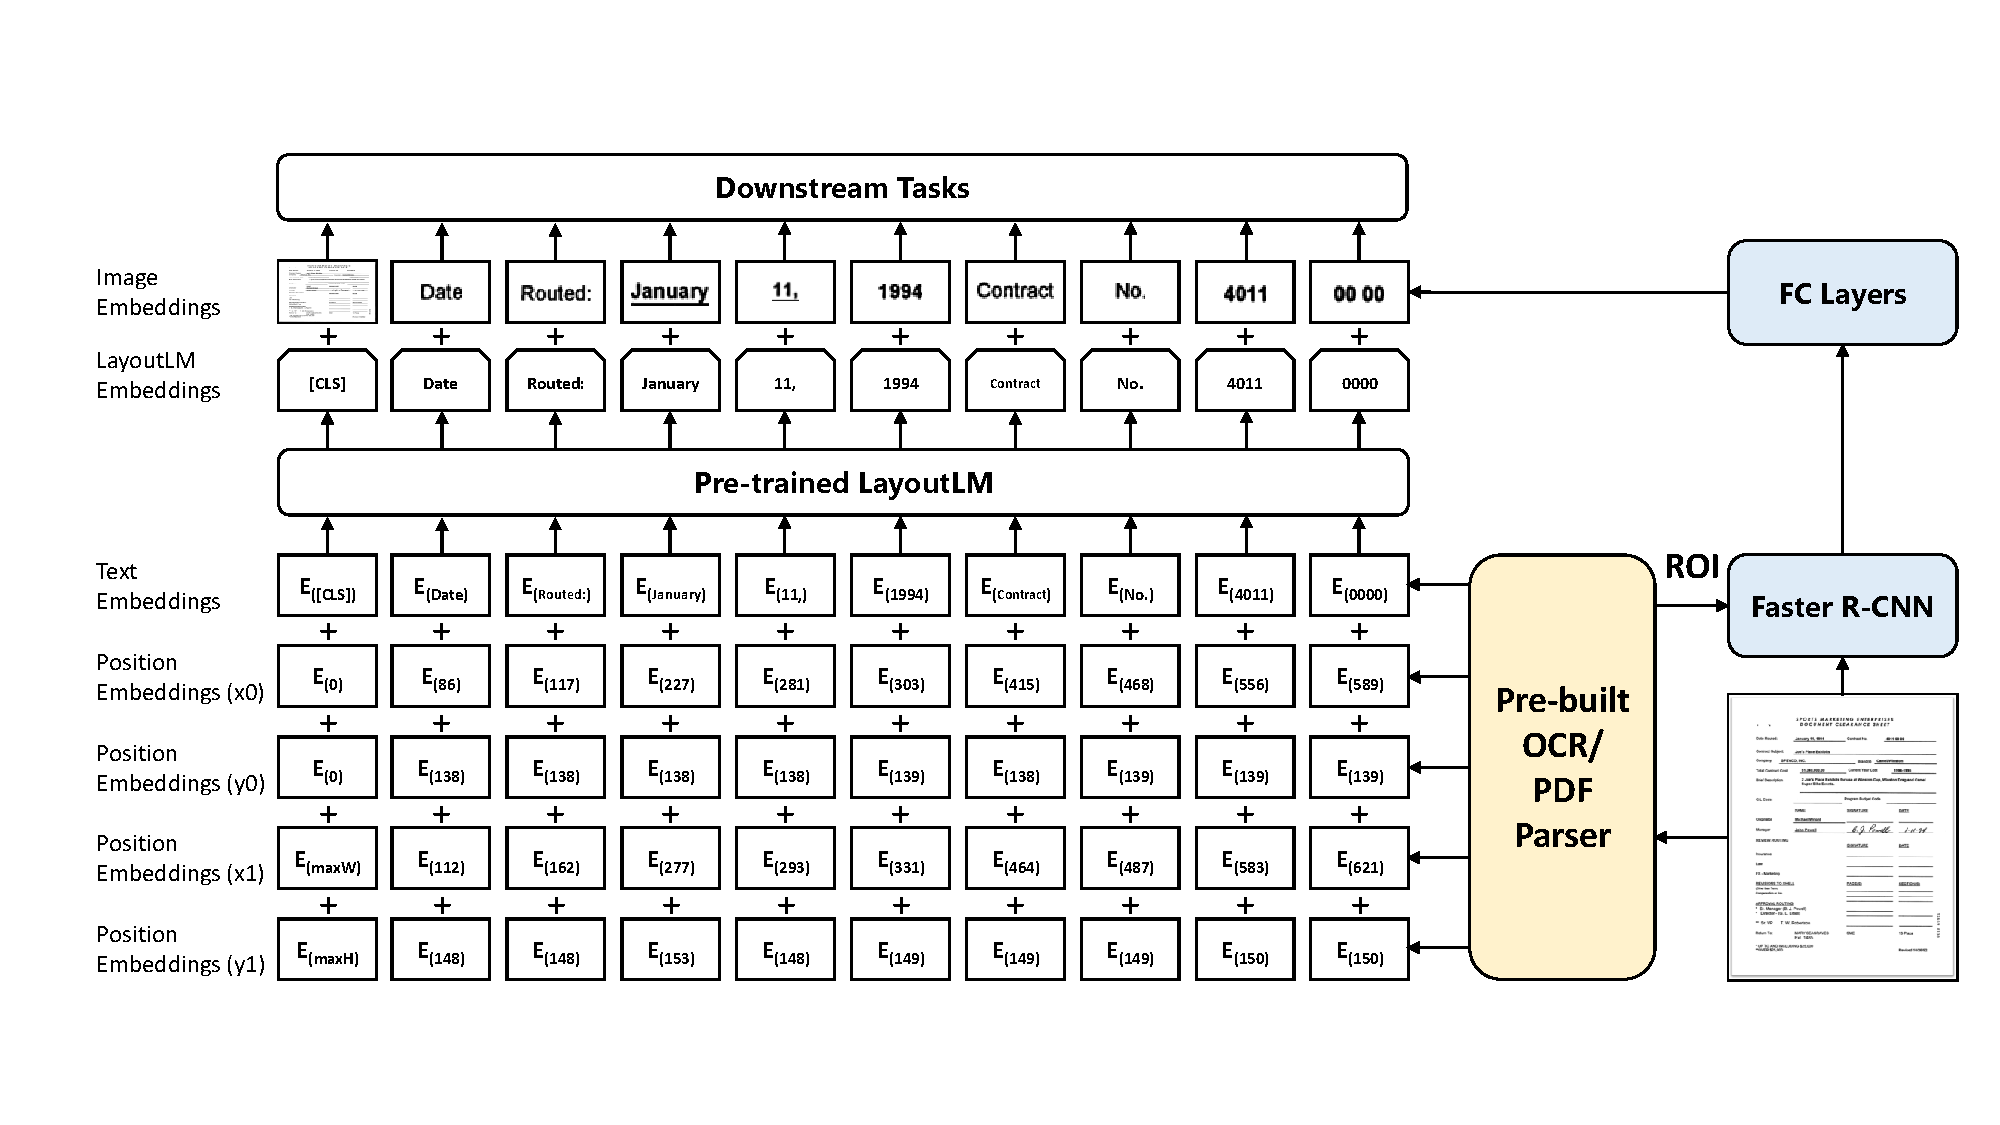
\includegraphics[width=0.80\textheight, angle=90]{img/layoutlm_arch.pdf}
  \caption*{Architecture du modèle multimodal LayoutLM (présentée en grand format horizontal). Extrait de \cite{xu_layoutlm_2020}.}
  \label{fig:layoutlm_annexe}
\end{figure}

\clearpage
% ---------------------------------------------------------------------
\subsection*{Annexe C - Matrice de confusion du modèle LayoutLM}
\addcontentsline{toc}{subsection}{Annexe C - Matrice de confusion de LayoutLM}
\label{ann:layoutlm_confusion}

\begin{figure}[H]
  \centering
  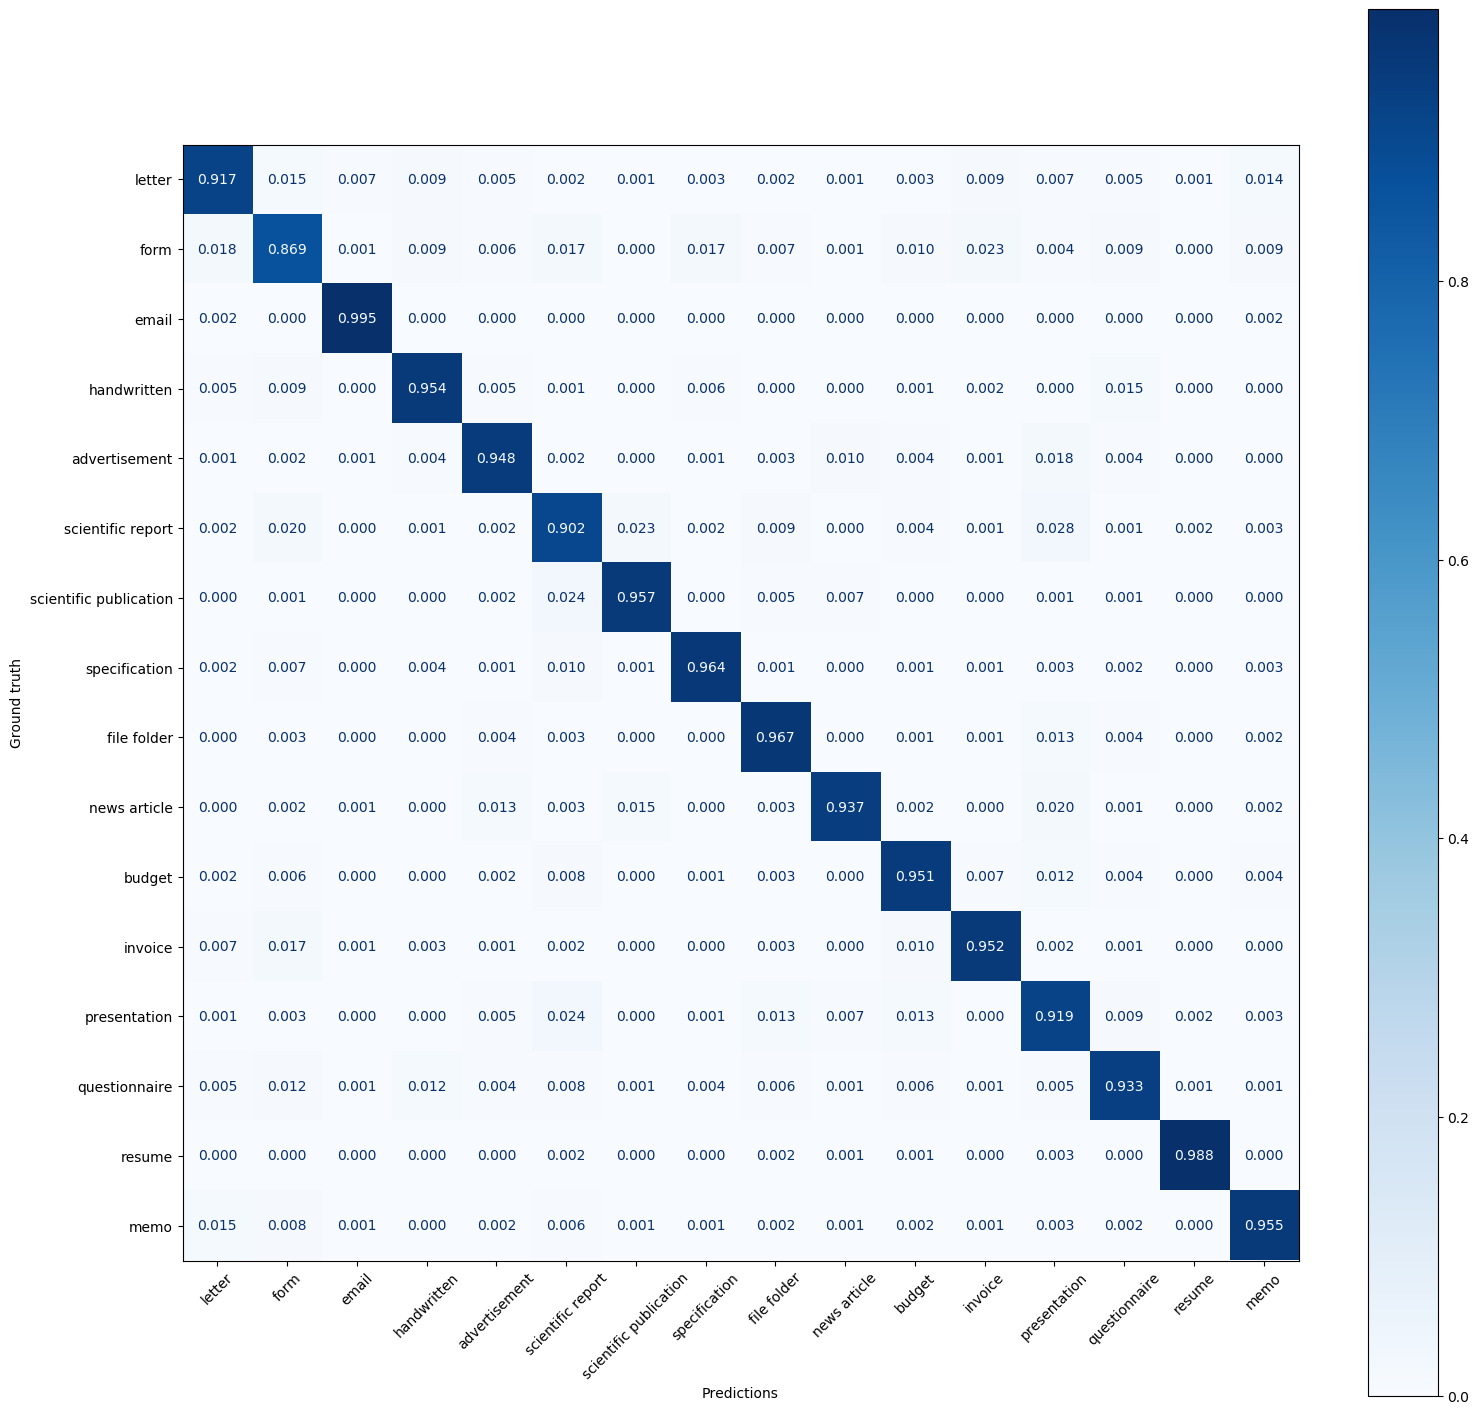
\includegraphics[width=0.80\textheight, angle=90]{img/layoutlm_confusion.png}
  \caption*{Matrice de confusion du modèle LayoutLM (présentée en grand format horizontal). Extrait de \cite{xu_layoutlm_2020}.}
  \label{fig:layoutlm_confusion_annexe}
\end{figure}

\clearpage

% ---------------------------------------------------------------------
\subsection*{Annexe D - Architecture globale du modèle GLiNER}
\addcontentsline{toc}{subsection}{Annexe D - Architecture de GLiNER}
\label{ann:gliner_architecture}

\begin{figure}[H]
  \centering
  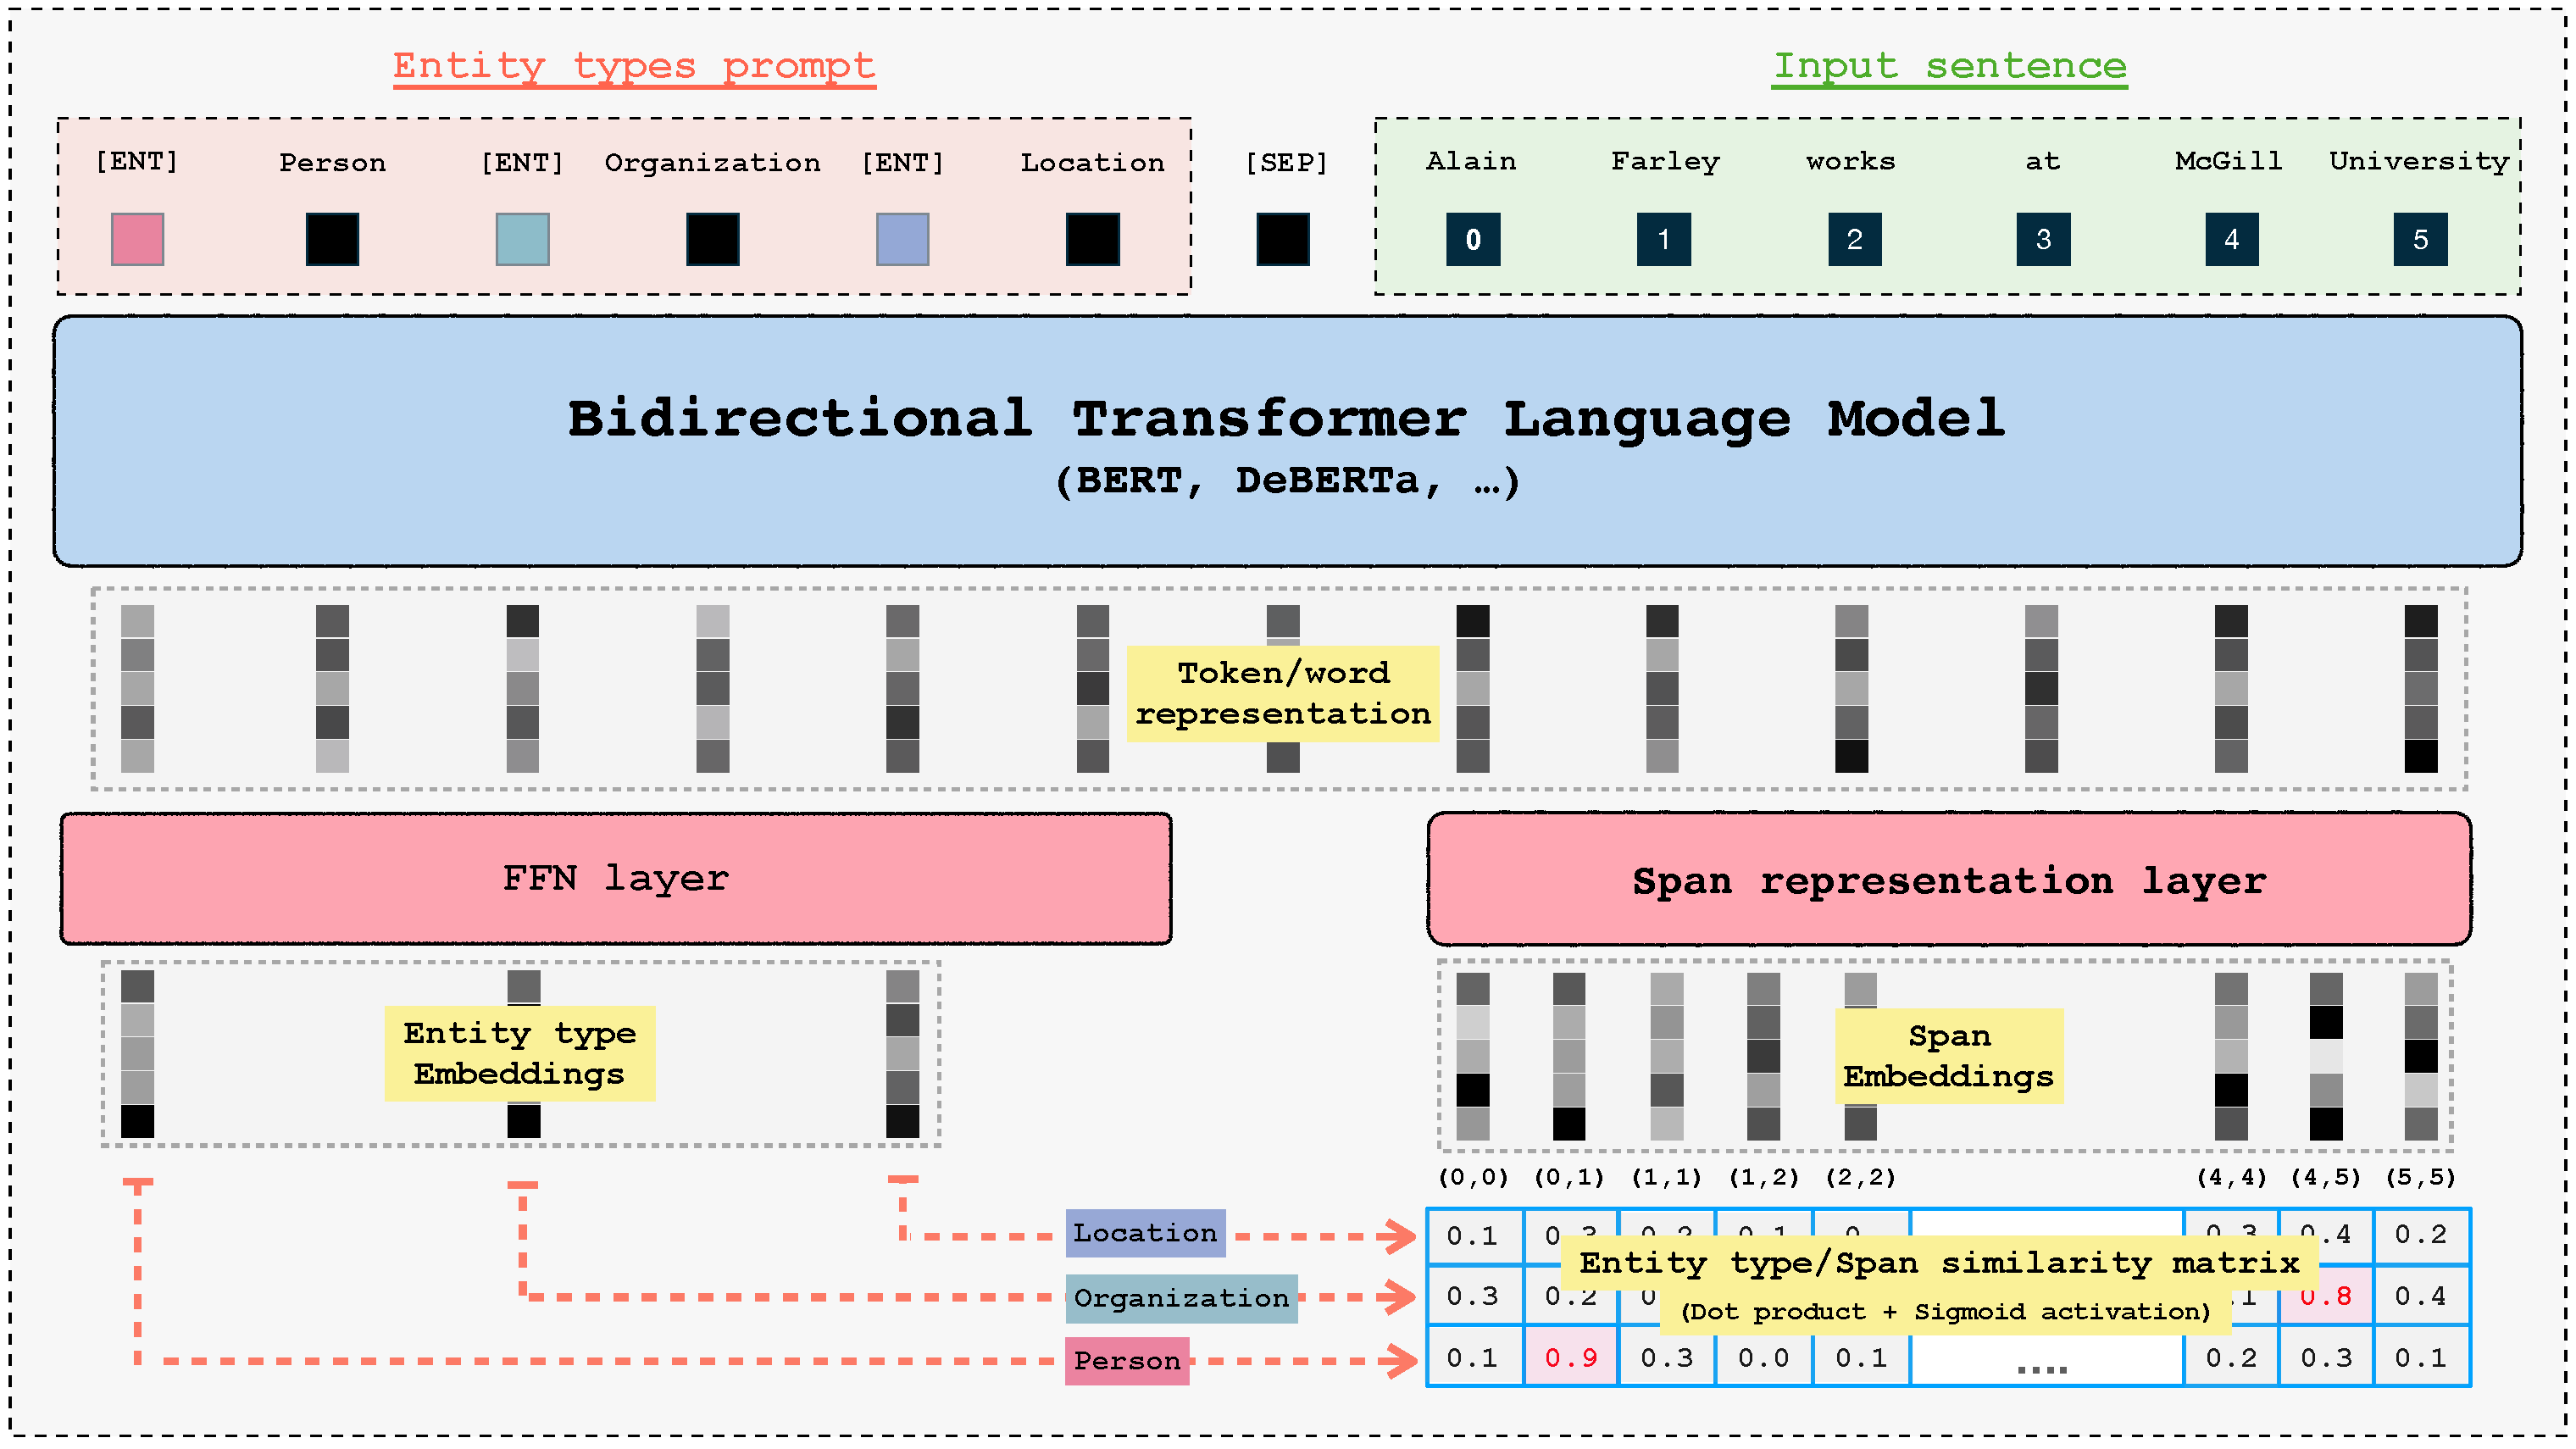
\includegraphics[width=0.80\textheight, angle=90]{img/gliner_gener.pdf}
  \caption*{Architecture globale du modèle GLiNER (présentée en grand format horizontal). Extrait de \cite{zaratiana_gliner_2024}.}
  \label{fig:gliner_annexe}
\end{figure}

\clearpage

% ---------------------------------------------------------------------
\subsection*{Annexe E - Architecture du modèle Vision-Langage LLaVA}
\addcontentsline{toc}{subsection}{Annexe E - Architecture de LLaVA}
\label{ann:llava_architecture}

\begin{figure}[H]
  \centering
  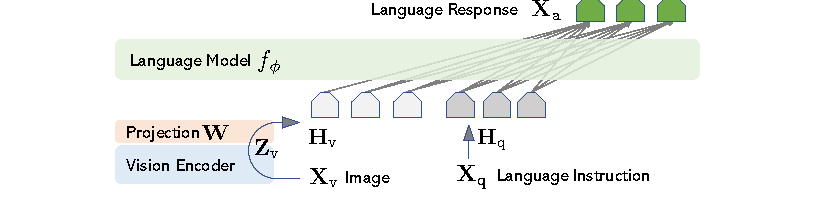
\includegraphics[width=0.80\textheight, angle=90]{img/llava_arch.pdf}
  \caption*{Architecture interne du modèle Vision-Langage LLaVA (présentée en grand format horizontal). Extrait de \cite{liu_llava_2024}.}
  \label{fig:llava_annexe}
\end{figure}

\clearpage

% ---------------------------------------------------------------------
\subsection*{Annexe F - Interface de validation du répertoire du Géomètre A}
\addcontentsline{toc}{subsection}{Annexe F - Interface du Géomètre A}
\label{ann:interface_geometre_a}

\begin{figure}[H]
  \centering
  \setlength{\fboxsep}{0pt}%
  \setlength{\fboxrule}{0.6pt}%
  \fbox{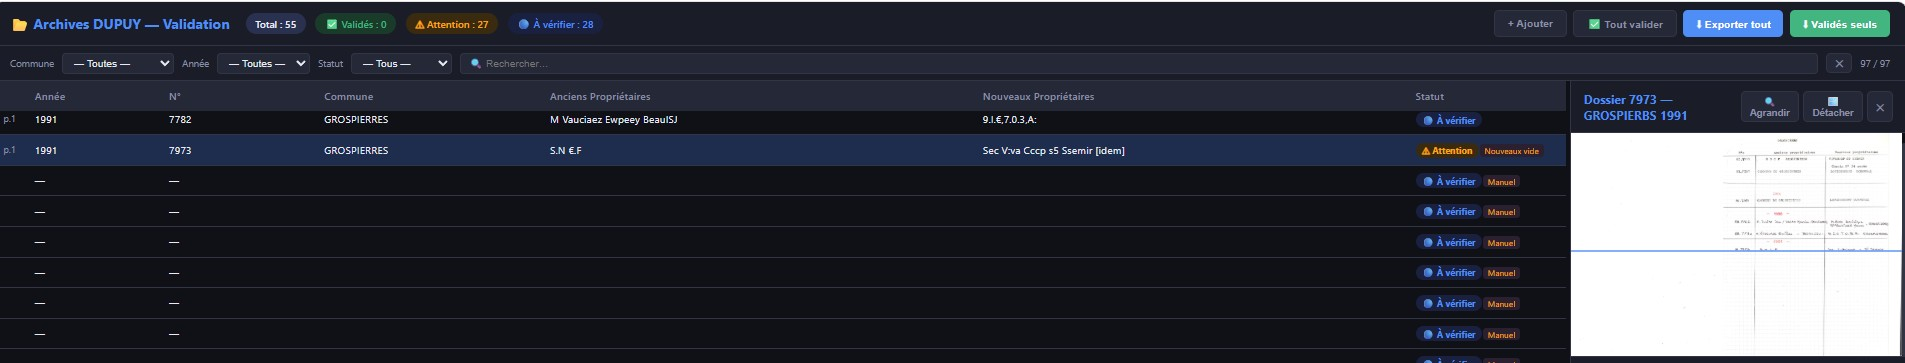
\includegraphics[width=0.94\textheight, keepaspectratio, angle=90]{img/5.5_reprtoire_A_liste.jpg}}
  \label{fig:interface_geometre_a_liste_annexe}
\end{figure}

\clearpage

\begin{figure}[H]
  \centering
  \setlength{\fboxsep}{0pt}%
  \setlength{\fboxrule}{0.6pt}%
  \fbox{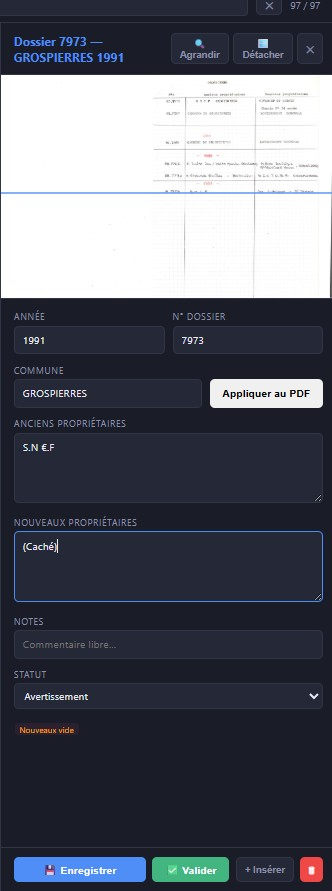
\includegraphics[height=0.82\textheight, keepaspectratio]{img/5.5_reprtoire_A_infos.jpg}}
  \caption*{Interface de validation du répertoire du Géomètre A (port 5050) -- Fiche détaillée et édition des champs (grand format).}
  \label{fig:interface_geometre_a_infos_annexe}
\end{figure}





\end{document}
